% Options for packages loaded elsewhere
\PassOptionsToPackage{unicode}{hyperref}
\PassOptionsToPackage{hyphens}{url}
%
\documentclass[
]{book}
\usepackage{amsmath,amssymb}
\usepackage{iftex}
\ifPDFTeX
  \usepackage[T1]{fontenc}
  \usepackage[utf8]{inputenc}
  \usepackage{textcomp} % provide euro and other symbols
\else % if luatex or xetex
  \usepackage{unicode-math} % this also loads fontspec
  \defaultfontfeatures{Scale=MatchLowercase}
  \defaultfontfeatures[\rmfamily]{Ligatures=TeX,Scale=1}
\fi
\usepackage{lmodern}
\ifPDFTeX\else
  % xetex/luatex font selection
\fi
% Use upquote if available, for straight quotes in verbatim environments
\IfFileExists{upquote.sty}{\usepackage{upquote}}{}
\IfFileExists{microtype.sty}{% use microtype if available
  \usepackage[]{microtype}
  \UseMicrotypeSet[protrusion]{basicmath} % disable protrusion for tt fonts
}{}
\makeatletter
\@ifundefined{KOMAClassName}{% if non-KOMA class
  \IfFileExists{parskip.sty}{%
    \usepackage{parskip}
  }{% else
    \setlength{\parindent}{0pt}
    \setlength{\parskip}{6pt plus 2pt minus 1pt}}
}{% if KOMA class
  \KOMAoptions{parskip=half}}
\makeatother
\usepackage{xcolor}
\usepackage{color}
\usepackage{fancyvrb}
\newcommand{\VerbBar}{|}
\newcommand{\VERB}{\Verb[commandchars=\\\{\}]}
\DefineVerbatimEnvironment{Highlighting}{Verbatim}{commandchars=\\\{\}}
% Add ',fontsize=\small' for more characters per line
\usepackage{framed}
\definecolor{shadecolor}{RGB}{248,248,248}
\newenvironment{Shaded}{\begin{snugshade}}{\end{snugshade}}
\newcommand{\AlertTok}[1]{\textcolor[rgb]{0.94,0.16,0.16}{#1}}
\newcommand{\AnnotationTok}[1]{\textcolor[rgb]{0.56,0.35,0.01}{\textbf{\textit{#1}}}}
\newcommand{\AttributeTok}[1]{\textcolor[rgb]{0.13,0.29,0.53}{#1}}
\newcommand{\BaseNTok}[1]{\textcolor[rgb]{0.00,0.00,0.81}{#1}}
\newcommand{\BuiltInTok}[1]{#1}
\newcommand{\CharTok}[1]{\textcolor[rgb]{0.31,0.60,0.02}{#1}}
\newcommand{\CommentTok}[1]{\textcolor[rgb]{0.56,0.35,0.01}{\textit{#1}}}
\newcommand{\CommentVarTok}[1]{\textcolor[rgb]{0.56,0.35,0.01}{\textbf{\textit{#1}}}}
\newcommand{\ConstantTok}[1]{\textcolor[rgb]{0.56,0.35,0.01}{#1}}
\newcommand{\ControlFlowTok}[1]{\textcolor[rgb]{0.13,0.29,0.53}{\textbf{#1}}}
\newcommand{\DataTypeTok}[1]{\textcolor[rgb]{0.13,0.29,0.53}{#1}}
\newcommand{\DecValTok}[1]{\textcolor[rgb]{0.00,0.00,0.81}{#1}}
\newcommand{\DocumentationTok}[1]{\textcolor[rgb]{0.56,0.35,0.01}{\textbf{\textit{#1}}}}
\newcommand{\ErrorTok}[1]{\textcolor[rgb]{0.64,0.00,0.00}{\textbf{#1}}}
\newcommand{\ExtensionTok}[1]{#1}
\newcommand{\FloatTok}[1]{\textcolor[rgb]{0.00,0.00,0.81}{#1}}
\newcommand{\FunctionTok}[1]{\textcolor[rgb]{0.13,0.29,0.53}{\textbf{#1}}}
\newcommand{\ImportTok}[1]{#1}
\newcommand{\InformationTok}[1]{\textcolor[rgb]{0.56,0.35,0.01}{\textbf{\textit{#1}}}}
\newcommand{\KeywordTok}[1]{\textcolor[rgb]{0.13,0.29,0.53}{\textbf{#1}}}
\newcommand{\NormalTok}[1]{#1}
\newcommand{\OperatorTok}[1]{\textcolor[rgb]{0.81,0.36,0.00}{\textbf{#1}}}
\newcommand{\OtherTok}[1]{\textcolor[rgb]{0.56,0.35,0.01}{#1}}
\newcommand{\PreprocessorTok}[1]{\textcolor[rgb]{0.56,0.35,0.01}{\textit{#1}}}
\newcommand{\RegionMarkerTok}[1]{#1}
\newcommand{\SpecialCharTok}[1]{\textcolor[rgb]{0.81,0.36,0.00}{\textbf{#1}}}
\newcommand{\SpecialStringTok}[1]{\textcolor[rgb]{0.31,0.60,0.02}{#1}}
\newcommand{\StringTok}[1]{\textcolor[rgb]{0.31,0.60,0.02}{#1}}
\newcommand{\VariableTok}[1]{\textcolor[rgb]{0.00,0.00,0.00}{#1}}
\newcommand{\VerbatimStringTok}[1]{\textcolor[rgb]{0.31,0.60,0.02}{#1}}
\newcommand{\WarningTok}[1]{\textcolor[rgb]{0.56,0.35,0.01}{\textbf{\textit{#1}}}}
\usepackage{longtable,booktabs,array}
\usepackage{calc} % for calculating minipage widths
% Correct order of tables after \paragraph or \subparagraph
\usepackage{etoolbox}
\makeatletter
\patchcmd\longtable{\par}{\if@noskipsec\mbox{}\fi\par}{}{}
\makeatother
% Allow footnotes in longtable head/foot
\IfFileExists{footnotehyper.sty}{\usepackage{footnotehyper}}{\usepackage{footnote}}
\makesavenoteenv{longtable}
\usepackage{graphicx}
\makeatletter
\def\maxwidth{\ifdim\Gin@nat@width>\linewidth\linewidth\else\Gin@nat@width\fi}
\def\maxheight{\ifdim\Gin@nat@height>\textheight\textheight\else\Gin@nat@height\fi}
\makeatother
% Scale images if necessary, so that they will not overflow the page
% margins by default, and it is still possible to overwrite the defaults
% using explicit options in \includegraphics[width, height, ...]{}
\setkeys{Gin}{width=\maxwidth,height=\maxheight,keepaspectratio}
% Set default figure placement to htbp
\makeatletter
\def\fps@figure{htbp}
\makeatother
\setlength{\emergencystretch}{3em} % prevent overfull lines
\providecommand{\tightlist}{%
  \setlength{\itemsep}{0pt}\setlength{\parskip}{0pt}}
\setcounter{secnumdepth}{5}
\ifLuaTeX
\usepackage[bidi=basic]{babel}
\else
\usepackage[bidi=default]{babel}
\fi
\babelprovide[main,import]{portuguese}
% get rid of language-specific shorthands (see #6817):
\let\LanguageShortHands\languageshorthands
\def\languageshorthands#1{}
\usepackage{booktabs}
\usepackage{amsthm}
\usepackage[T1]{fontenc}
\usepackage[utf8]{inputenc}
\usepackage{lmodern}
\usepackage[brazil]{babel}
\usepackage[left=3cm,right=2cm,top=2cm,bottom=2cm]{geometry}
\makeatletter
\def\thm@space@setup{%
  \thm@preskip=8pt plus 2pt minus 4pt
  \thm@postskip=\thm@preskip
}
\makeatother
\ifLuaTeX
  \usepackage{selnolig}  % disable illegal ligatures
\fi
\usepackage[]{natbib}
\bibliographystyle{apalike}
\usepackage{bookmark}
\IfFileExists{xurl.sty}{\usepackage{xurl}}{} % add URL line breaks if available
\urlstyle{same}
\hypersetup{
  pdftitle={Estatística + R},
  pdfauthor={Ana Paula Fernandes (DESCO/UFTM)},
  pdflang={pt},
  hidelinks,
  pdfcreator={LaTeX via pandoc}}

\title{Estatística + R}
\author{Ana Paula Fernandes (DESCO/UFTM)}
\date{Atualizado em: 01/06/2025}

\begin{document}
\maketitle

{
\setcounter{tocdepth}{1}
\tableofcontents
}
\chapter{Bem-vindos!}\label{bem-vindos}

Esse livro \emph{online} tem como propósito principal ser um guia para as aulas de estatística, referente as disciplinas de \textbf{Bioestatística} para os curso de Medicina e Educação Física e \textbf{Estatística Aplicada} para o curso de Psicologia da \href{http://www.uftm.edu.br}{Universidade Federal do Triângulo Mineiro - UFTM}. E como objetivo secundário, ser uma referência de consulta para todos os discentes que passaram por essas disciplinas, bem como, para todos que estão interessados em realizar análises de dados por meio da linguagem R e o ambiente de desenvolvimento RStudio.

Sugestões, correções ou qualquer outra forma de interação são sempre bem-vindas! Então, por favor, não hesite em me escrever (\href{mailto:anapaula.fernandes@uftm.edu.br}{\nolinkurl{anapaula.fernandes@uftm.edu.br}}).

Para mais informações sobre minha trajetória acadêmica e profissional, acesse meu \href{https://lattes.cnpq.br/5582801060910261}{Currículo Lattes}.

\chapter{Introdução}\label{intro}

Ao longo de algum tempo ministrando aulas de estatísticas conclui que estudar estatística com auxílio de recursos computacionais é bem mais eficaz, quero dizer, é mais fácil entender os conceitos téoricos, lidar com recusos visuais (gráficos) e, de fato, transformar o contéudo estudado na disciplina em uma ferramenta para pesquisas científicas, quando se trata de analisar dados.

Ministrando aulas para os cursos da área de saúde, esporte e psicologia sempre ouvi dos discentes que estatística é matemática, e sempre digo que estatística é estatística! É normal alguns discentes não assimilarem, em princípio, a importância da disciplina na grade do seu curso, e realmente, alguns acham até que é assunto que deveria ficar restrito aos curso das exatas. Assim, a primeira tarefa é sempre desconstruir essa ideia.

A estatística é \textbf{MULTIDICIPLINAR}, ela está em tudo na verdade\ldots{} e para dizer uma coisa ``bem chique'' a estatística é a base da Inteligência Artificial. Advinha quem está por trás dos famosos algortimos das redes sociais? Ou das sugestões de filmes e músicas que aparecem no seu \emph{streamming} favorito? Ou no ranque de busca realzada por meio do \emph{Google}? Ou no \emph{Chat} GTP?

E sendo um pouco mais ``acadêmica'', dentro do nosso propósito:

Qualquer competição ou treinamento esportivo está recheado de estatística, como medir o desempenho de um time ou atleta? Veja esse exemplo aqui:

\begin{quote}
\textbf{Velocidade e resistência de velocidade de sprint em atletas de Futebol amador} \url{http://www.rbff.com.br/index.php/rbff/article/view/866}
\end{quote}

Na medicina, estudos epidemiologicos, e claro, da medicina baseada em evidências, tem o suporte da estatística. Veja esse exemplo aqui:

\begin{quote}
\textbf{Qualidade de Vida Relacionada à Saúde e Satisfação com o Tratamento Hospitalar de Adultos com Câncer: Estudo Observacional} \url{https://rbc.inca.gov.br/index.php/revista/article/view/3554}
\end{quote}

Na psicologia a estatística é a ferramenta utilizada na psicometria. Veja esse exemplo:

\begin{quote}
\textbf{Escala de Comportamentos Antissociais: construção e estudos psicométricos} \url{https://periodicos.pucpr.br/psicologiaargumento/article/view/27071}
\end{quote}

Basta realizar uma busca com os termos estatística e um campo do seu curso que você se interessa, que você encontrará um artigo científico. E se você não encontrar, comece a escreve sobre o tema!

Quando olhamos os artigos acima, podemos ver que todos eles tem resultados \textbf{descritivos} e \textbf{inferenciais}. Discutiremos sobre estatística descritiva (de descrever - os dados amostrados para uma dada análise) e inferencial (de inferir - tirar conclusões a partir dos dados amostrados) no próximo tópico.

\section{Atividade 1}\label{atividade-1}

\textbf{Busque um artigo do campo de seu interesse que utiliza a estatística.}

\begin{enumerate}
\def\labelenumi{\arabic{enumi}.}
\tightlist
\item
  \textbf{Qual é o principal objetivo da pesquisa?}

  \begin{itemize}
  \tightlist
  \item
    Qual é a questão central que a pesquisa busca responder? Os autores apresentam claramente os objetivos do estudo e o que se espera alcançar com os resultados?
  \end{itemize}
\item
  \textbf{Como a pesquisa foi conduzida?}

  \begin{itemize}
  \tightlist
  \item
    Quais métodos foram utilizados para coletar os dados? A pesquisa é qualitativa ou quantitativa? Os autores descrevem o procedimento de forma detalhada, incluindo a amostra, os instrumentos de coleta de dados e a análise estatística realizada?
  \end{itemize}
\item
  \textbf{O que é apresentado por meio de tabelas ou gráficos?}

  \begin{itemize}
  \tightlist
  \item
    Quais informações estão sendo representadas visualmente? Os gráficos e tabelas são claros e bem organizados para facilitar a compreensão dos dados? Como os resultados são interpretados a partir dessas representações?
  \end{itemize}
\item
  \textbf{Faça uma lista de termos relacionados à estatística encontrados no artigo.}

  \begin{itemize}
  \tightlist
  \item
    Identifique e liste os termos e conceitos estatísticos mencionados no artigo. Isso pode incluir testes de hipótese, modelos estatísticos, variáveis dependentes e independentes, intervalos de confiança, p-valor, etc.
  \end{itemize}
\end{enumerate}

\begin{quote}
Periódicos da área da Ciência dos Esportes
\end{quote}

\begin{itemize}
\item
  RBFF - Revista Brasileira de Futsal e Futebol \url{http://www.rbff.com.br}
\item
  RBME - Revista Brasileira de Medicina do Esporte \url{https://www.scielo.br/j/rbme}
\item
  RBPE - Revista Brasileira de Psicologia do Esporte \url{http://pepsic.bvsalud.org}
\end{itemize}

\begin{quote}
Periódicos da área de Medicina
\end{quote}

\begin{itemize}
\item
  RBC - Revista Brasileira de Cancerologia \url{https://rbc.inca.gov.br/index.php/revista}
\item
  RBCMS - Revista Brasileira de Ciências Médicas e da Saúde \url{http://www.rbcms.com.br}
\item
  Revista da Associação Brasileira de Saúde Coletiva \url{https://cienciaesaudecoletiva.com.br}
\end{itemize}

\begin{quote}
Periódicos da área de Piscologia
\end{quote}

\begin{itemize}
\item
  Psicologia argumento \url{https://periodicos.pucpr.br/psicologiaargumento}
\item
  Estudos de psicologia (Campinas) \url{https://www.scielo.br/j/estpsi/}
\item
  Psicologia em foco \url{https://revistas.fw.uri.br/index.php/psicologiaemfoco}
\end{itemize}

\begin{quote}
Ou busque na ferramenta \emph{Mendeley} \url{https://www.mendeley.com}
\end{quote}

\chapter{Definições Iniciais}\label{definiuxe7uxf5es-iniciais}

A \textbf{Estatística} é uma área fundamental para entender e analisar dados de diversas áreas do conhecimento.

\section{Estatística Descritiva}\label{estatuxedstica-descritiva}

\subsection{\texorpdfstring{Exemplo 1: \textbf{Saúde Mental dos Estudantes}}{Exemplo 1: Saúde Mental dos Estudantes}}\label{exemplo-1-sauxfade-mental-dos-estudantes}

Suponha que você deseje realizar uma pesquisa na UFTM para avaliar a saúde mental dos estudantes. Os dados coletados provavelmente incluirão informações sobre os níveis de \textbf{estresse}, \textbf{ansiedade}, \textbf{depressão} e \textbf{bem-estar geral} dos alunos. Nesse contexto, a \textbf{Estatística Descritiva} seria uma ferramenta essencial para organizar esses dados e apresentá-los de maneira clara, objetiva e compreensível.

Utilizando a Estatística Descritiva, você poderia:

\begin{enumerate}
\def\labelenumi{\arabic{enumi}.}
\tightlist
\item
  \textbf{Organizar e estruturar os dados}, criando tabelas que agrupem as respostas dos estudantes de forma sistemática, o que facilitaria a análise dos padrões e a visualização de tendências.
\item
  \textbf{Calcular medidas de tendência central}, como a \textbf{média} dos níveis de estresse ou ansiedade, permitindo que você obtenha uma visão geral dos aspectos mais comuns da saúde mental entre os estudantes.
\item
  \textbf{Elaborar gráficos}, como \textbf{gráficos de barras} ou \textbf{diagramas de caixa}, para representar visualmente os dados e facilitar a interpretação. Por exemplo, esses gráficos poderiam mostrar quantos alunos estão em diferentes faixas de intensidade de ansiedade (baixo, moderado ou alto).
\item
  \textbf{Calcular medidas de dispersão}, como o \textbf{desvio padrão}, para avaliar a variabilidade dos dados. Um desvio padrão alto, por exemplo, indicaria que há uma grande diferença entre os níveis de estresse ou ansiedade dos estudantes, o que poderia apontar para a necessidade de abordagens personalizadas em programas de apoio.
\item
  \textbf{Identificar padrões e correlações} nos dados, como a relação entre o nível de estresse e o número de horas de estudo, ou entre o bem-estar geral e a prática de atividades físicas, ajudando a identificar fatores que influenciam a saúde mental dos estudantes.
\end{enumerate}

Essas análises permitiriam que você compreendesse melhor o panorama da saúde mental dos alunos da UFTM e fornecesse uma base sólida para tomar decisões informadas sobre possíveis ações e programas de apoio psicológico.

\subsection{\texorpdfstring{Exemplo 2: \textbf{Prática de Atividades Físicas}}{Exemplo 2: Prática de Atividades Físicas}}\label{exemplo-2-pruxe1tica-de-atividades-fuxedsicas}

Se o objetivo for entender a frequência com que os estudantes da UFTM praticam atividades físicas regularmente, podemos coletar dados específicos, como:

\begin{itemize}
\item
  \textbf{Percentual de alunos que praticam esportes regularmente}: A porcentagem de estudantes que praticam atividades físicas \textbf{mais de três vezes por semana}. Este dado oferece uma visão geral sobre a adesão à prática de exercícios e pode ser útil para identificar possíveis áreas de melhoria no incentivo à saúde física.
\item
  \textbf{Distribuição por tipo de atividade física}: Podemos utilizar gráficos como \textbf{gráficos de pizza} ou \textbf{barras empilhadas} para mostrar a diversidade de atividades praticadas pelos estudantes. Por exemplo, os gráficos poderiam ilustrar a proporção de alunos que praticam \textbf{corrida}, \textbf{musculação}, \textbf{dança}, \textbf{futebol}, entre outras atividades, permitindo uma visão clara sobre as preferências esportivas da comunidade acadêmica.
\item
  \textbf{Intensidade da prática de atividades físicas}: Coletar dados sobre a intensidade das atividades (leve, moderada ou intensa) também seria relevante, pois ajudaria a universidade a entender não só a frequência, mas também o impacto potencial dessas atividades na saúde física e mental dos estudantes.
\end{itemize}

Essas informações não apenas proporcionam um panorama claro sobre o comportamento dos estudantes em relação à saúde física, mas também podem embasar a criação de novos programas e campanhas para incentivar a prática de atividades físicas, promovendo o bem-estar geral da comunidade acadêmica.

\section{Estatística Inferencial}\label{estatuxedstica-inferencial}

\subsection{\texorpdfstring{Exemplo 1: \textbf{Saúde Mental dos Estudantes}}{Exemplo 1: Saúde Mental dos Estudantes}}\label{exemplo-1-sauxfade-mental-dos-estudantes-1}

Suponha que você queira avaliar a saúde mental dos estudantes da UFTM e, para isso, tenha realizado uma pesquisa com uma amostra de 200 estudantes. Neste caso, a \textbf{Estatística Inferencial} será uma ferramenta essencial para generalizar os resultados dessa amostra para toda a população de estudantes da universidade.

\begin{itemize}
\item
  \textbf{Estimativa da média de ansiedade}: Se a média da amostra indicar que os estudantes têm um nível de ansiedade de 7 (em uma escala de 0 a 10), a Estatística Inferencial permitirá que você estime o nível médio de ansiedade de todos os estudantes da UFTM. A partir dessa amostra, podemos calcular um \textbf{intervalo de confiança}, que nos dirá com que precisão a média da amostra reflete a média da população inteira. Isso nos dá uma estimativa com uma margem de erro, ajudando a compreender a variabilidade e a precisão do resultado.
\item
  \textbf{Testes de hipóteses}: Suponha que você queira comparar os níveis de ansiedade entre estudantes de diferentes cursos. Por exemplo, você deseja saber se os estudantes do curso de Medicina apresentam níveis de ansiedade significativamente mais altos do que os estudantes do curso de Engenharia. A Estatística Inferencial permite realizar um \textbf{teste de hipótese}, que nos ajuda a determinar se a diferença observada entre as médias dos dois grupos é \textbf{estatisticamente significativa} ou se pode ter ocorrido por acaso. Isso nos permite tomar decisões informadas sobre possíveis relações entre variáveis, com base em dados e não em suposições.
\end{itemize}

Esses exemplos demonstram como a Estatística Inferencial pode ser usada para tirar conclusões sobre toda a população de estudantes da UFTM, com base em uma amostra representativa. Isso é essencial para planejar intervenções e políticas de apoio à saúde mental de forma mais eficaz.

\subsection{\texorpdfstring{Exemplo 2: \textbf{Prática de Atividades Físicas}}{Exemplo 2: Prática de Atividades Físicas}}\label{exemplo-2-pruxe1tica-de-atividades-fuxedsicas-1}

Suponha que você esteja interessado em saber como os hábitos de atividade física variam entre os cursos da UFTM. A universidade realiza uma pesquisa com uma amostra de 300 estudantes, incluindo alunos de Medicina e de Educação Física. A \textbf{Estatística Inferencial} pode ser usada para tirar conclusões sobre toda a população de estudantes com base nessa amostra.

\begin{itemize}
\item
  \textbf{Estimar a proporção de estudantes ativos fisicamente}: Se 60\% dos estudantes da amostra afirmam praticar atividades físicas regularmente, podemos usar a \textbf{probabilidade} para estimar a proporção de todos os estudantes da UFTM que têm esse hábito. A partir desses dados, também é possível calcular um \textbf{intervalo de confiança}, indicando com que precisão essa estimativa reflete a realidade da população.
\item
  \textbf{Comparação entre cursos}: Podemos realizar um \textbf{teste de comparação de proporções} para verificar se a prática de atividades físicas é mais frequente entre estudantes de Educação Física do que entre estudantes de Medicina. Esse teste nos ajudaria a determinar se a diferença observada entre os dois cursos é estatisticamente significativa ou se pode ser explicada por variações aleatórias.
\end{itemize}

Essas análises ajudam a universidade a entender os padrões de comportamento relacionados à saúde física entre diferentes grupos acadêmicos e a planejar ações mais específicas para incentivar o bem-estar entre os estudantes.

\section{Conexão com a Probabilidade}\label{conexuxe3o-com-a-probabilidade}

Esses dois tipos de análise estão profundamente conectados com a \textbf{Teoria de Probabilidade}, que nos permite estimar as chances de um evento acontecer e tomar decisões com base nesses dados. No caso da UFTM, podemos usar a \textbf{probabilidade} para prever, por exemplo, a chance de um estudante desenvolver sintomas de estresse durante o semestre, com base em comportamentos anteriores, como hábitos de estudo e participação em atividades de lazer.

\section{População x Amostra}\label{populauxe7uxe3o-x-amostra}

\subsection{\texorpdfstring{\textbf{População}}{População}}\label{populauxe7uxe3o}

A \textbf{população} é o conjunto completo de indivíduos que queremos estudar. No contexto de uma pesquisa com estudantes da UFTM, a população pode ser definida como \textbf{todos os 6.900 estudantes} da instituição, considerando alunos da graduação, cursos técnicos e pós-graduação (dados do DRCA, em dezembro de 2024).

\subsection{\texorpdfstring{\textbf{Amostra}}{Amostra}}\label{amostra}

Uma \textbf{amostra} é um grupo menor selecionado dessa população, que deve ser representativo o suficiente para permitir inferências sobre o todo. Por exemplo, em vez de aplicar um questionário para todos os 6.900 estudantes, podemos selecionar uma \textbf{amostra aleatória de 364 estudantes}.

Esse tamanho de amostra é adequado para garantir um \textbf{erro máximo de 5\%}, com \textbf{95\% de confiança} nos resultados. Isso significa que, com essa amostra, conseguimos estimar com boa precisão como é a situação da saúde dos estudantes da universidade como um todo.

\subsection{\texorpdfstring{\textbf{Exemplo aplicado}}{Exemplo aplicado}}\label{exemplo-aplicado}

Suponha que você queira avaliar o nível de bem-estar emocional dos estudantes da UFTM. Você aplica um questionário padronizado para uma amostra aleatória de \textbf{364 estudantes}. A partir das respostas, você calcula que a média de bem-estar emocional, numa escala de 0 a 10, é \textbf{6,8}.

Com esse resultado e a ajuda da \textbf{estatística inferencial}, você pode estimar com segurança que o nível médio de bem-estar emocional da \textbf{população inteira} de estudantes da UFTM está próximo de \textbf{6,8}, com uma \textbf{margem de erro de 5\%}.

Isso significa que, com \textbf{95\% de confiança}, o \textbf{intervalo de confiança} para a média do bem-estar emocional está entre \textbf{6,46 e 7,14}. Em outras palavras, se essa pesquisa fosse repetida várias vezes com diferentes amostras aleatórias de 364 estudantes, em 95\% das vezes o valor da média real da população estaria dentro desse intervalo.

\chapter{Tamanho da Amostra}\label{tamanho-da-amostra}

O cálculo do \textbf{tamanho da amostra} é um passo importante em qualquer pesquisa. Ele nos ajuda a determinar quantos participantes precisamos para que os resultados sejam representativos e estatisticamente confiáveis. Embora o cálculo envolva alguns conceitos de \textbf{estatística inferencial}, hoje em dia, esse processo pode ser muito mais simples, graças a ferramentas online e até mesmo com o auxílio de \textbf{Inteligência Artificial (IA)}.

\section{Passos básicos para o cálculo do tamanho da amostra}\label{passos-buxe1sicos-para-o-cuxe1lculo-do-tamanho-da-amostra}

Quando o objetivo é estimar uma proporção, o cálculo do tamanho amostral exige algumas informações essenciais:

\begin{enumerate}
\def\labelenumi{\arabic{enumi}.}
\tightlist
\item
  \textbf{Tamanho da população}: Neste caso, os estudantes da UFTM, que somam cerca de \textbf{6.900}.
\item
  \textbf{Margem de erro}: A precisão com que queremos que nossa estimativa esteja próxima da realidade. Por exemplo, uma margem de erro de \textbf{5\%} é comum em muitos estudos.
\item
  \textbf{Nível de confiança}: Normalmente, utiliza-se 95\%, que indica a probabilidade de que o intervalo de confiança contenha o valor real.
\end{enumerate}

A fórmula para calcular o tamanho da amostra é:

\[
n = \frac{{Z^2 \cdot p \cdot (1 - p)}}{{E^2}}
\]

Onde:
- \(n\) = tamanho da amostra
- \(Z\) = valor da distribuição normal (geralmente 1,96 para 95\% de confiança)
- \(p\) = proporção estimada (por exemplo, 0,5 para o pior cenário)
- \(E\) = margem de erro (por exemplo, 0,05 para 5\%)

\section{Exemplo de cálculo simples}\label{exemplo-de-cuxe1lculo-simples}

Vamos calcular o tamanho da amostra para uma pesquisa na UFTM, onde sabemos que a população tem \textbf{6.900 estudantes}, a margem de erro é \textbf{5\%}, o nível de confiança é \textbf{95\%}, e vamos supor que queremos estimar uma proporção de \textbf{50\%} (o pior cenário para garantir maior precisão).

Usando a fórmula, temos:

\begin{itemize}
\tightlist
\item
  \(Z = 1,96\) (para 95\% de confiança)
\item
  \(p = 0,5\) (proporção estimada)
\item
  \(E = 0,05\) (margem de erro de 5\%)
\end{itemize}

Substituindo os valores na fórmula, obtemos:

\[
n = \frac{{1,96^2 \cdot 0,5 \cdot (1 - 0,5)}}{{0,05^2}} = 384
\]

Logo, o tamanho da amostra necessário é \textbf{384} estudantes para garantir uma margem de erro de 5\% com 95\% de confiança.

\textbf{Observação:} A fórmula apresentada acima é utilizada para o cálculo do tamanho amostral quando se deseja estimar uma proporção, assumindo uma população infinita (ou muito grande). Para situações em que o objetivo é estimar a média populacional, a fórmula adequada é diferente e leva em conta o desvio padrão da variável em vez da proporção. Além disso, se a população for finita, é necessário aplicar o fator de correção amostral.

\subsection{Ferramentas para cálculo de amostra}\label{ferramentas-para-cuxe1lculo-de-amostra}

Nosso foco aqui não é ensinar a fazer os cálculos manualmente, mas compreender os conceitos envolvidos. Existem diversas ferramentas online gratuitas que fazem o cálculo automaticamente. Por exemplo:

\section{Cálculo do Tamanho da Amostra}\label{cuxe1lculo-do-tamanho-da-amostra}

Para calcular o tamanho da amostra, podemos utilizar diferentes ferramentas, tanto no \textbf{R} quanto online. Aqui estão algumas opções:

\begin{itemize}
\item
  \textbf{No R}: Para calcular o tamanho da amostra, podemos utilizar o \textbf{pacote pwr}, que oferece funções específicas para realizar esses cálculos de forma simples e eficaz. O pacote é ideal para quem precisa calcular o tamanho da amostra para testes de hipóteses, como testes de médias, proporções ou análise de variância, ajustando facilmente os parâmetros conforme as necessidades da pesquisa.
\item
  \textbf{Calculadora Amostral Online da USP Bauru}: \href{http://estatistica.bauru.usp.br/calculoamostral/}{Clique aqui para acessar} - Uma ferramenta simples e eficiente para cálculos amostrais.
\item
  \textbf{G*Power}: Um software gratuito que pode ajudar a calcular o tamanho da amostra dependendo do tipo de análise estatística que você irá realizar. \href{https://www.gpower.hhu.de/en.html}{Saiba mais sobre o G*Power}.
\item
  \textbf{OpenEpi -- Sample Size}: \href{https://www.openepi.com/SampleSize/SSMean.htm}{Acesse aqui} - Muito usado na área da saúde, permite calcular amostras para média, proporção, estudos de caso-controle, coorte, entre outros.
\end{itemize}

\subsection{Conclusão}\label{conclusuxe3o}

Em resumo, o cálculo do \textbf{tamanho da amostra} é um passo essencial para garantir que suas pesquisas sejam precisas e representativas. Embora os cálculos possam parecer complexos, hoje em dia, existem ferramentas poderosas e \textbf{Inteligência Artificial} para facilitar esse processo, economizando tempo e esforço na sua pesquisa.

\section{Atividade 2}\label{atividade-2}

\textbf{Responda a partir do artigo buscado na atividade 1.}

\begin{enumerate}
\def\labelenumi{\arabic{enumi}.}
\tightlist
\item
  \textbf{Os autores discutem o cálculo do tamanho da amostra no estudo?}

  \begin{itemize}
  \tightlist
  \item
    Você consegue identificar se os autores fornecem uma explicação clara sobre como determinaram o tamanho da amostra na pesquisa? Eles utilizaram alguma fórmula específica ou ferramenta estatística para esse cálculo?
  \end{itemize}
\item
  \textbf{A população da pesquisa foi claramente definida pelos autores?}

  \begin{itemize}
  \tightlist
  \item
    Os autores descreveram com clareza quem compõe a população da pesquisa (por exemplo, características demográficas, contexto da amostra, entre outros)? A população foi bem delineada para garantir que os resultados sejam representativos?
  \end{itemize}
\item
  \textbf{O tamanho da amostra utilizado no estudo foi adequado?}

  \begin{itemize}
  \tightlist
  \item
    Com base no cálculo do tamanho de amostra, você acha que a amostra utilizada no estudo foi grande o suficiente para garantir a precisão dos resultados? Ela foi suficientemente representativa da população alvo da pesquisa?
  \end{itemize}
\item
  \textbf{Realize o cálculo do tamanho de amostra para este estudo.}

  \begin{itemize}
  \tightlist
  \item
    Com as informações fornecidas pelos autores, você pode calcular o tamanho da amostra necessário para o estudo utilizando uma fórmula ou ferramenta de cálculo amostral. Considere aspectos como o nível de confiança, margem de erro e variabilidade dos dados.
  \end{itemize}
\item
  \textbf{Os autores mencionaram se a pesquisa foi aprovada pelo Comitê de Ética?}

  \begin{itemize}
  \tightlist
  \item
    No artigo, há alguma referência sobre a aprovação ética da pesquisa? Os autores informaram se a pesquisa foi submetida e aprovada por um Comitê de Ética em Pesquisa (CEP)?
  \end{itemize}
\item
  \textbf{Qual é a importância de submeter a pesquisa ao Comitê de Ética?}

  \begin{itemize}
  \tightlist
  \item
    Por que é essencial que a pesquisa seja submetida a um Comitê de Ética? Quais são as implicações éticas de não realizar essa submissão, especialmente em pesquisas que envolvem seres humanos?
  \end{itemize}
\end{enumerate}

\textbf{Importante}

\begin{quote}
Conheça o Comitê de Ética em Pesquisa (CEP) da UFTM
\end{quote}

\url{https://www.uftm.edu.br/comitesecomissoes/cep}

\chapter{Técnicas de Amostragem}\label{tuxe9cnicas-de-amostragem}

Em pesquisas, uma das etapas mais importantes é o \textbf{cálculo amostral}, que determina quantos participantes serão necessários para garantir que os resultados sejam confiáveis. Depois, é preciso escolher uma \textbf{técnica de amostragem}, ou seja, como vamos selecionar as pessoas ou unidades que farão parte da pesquisa. Uma parte essencial disso é garantir que o processo de amostragem evite \textbf{viés}, que ocorre quando a amostra não representa adequadamente a população.

Existem várias técnicas de amostragem, cada uma com suas características, vantagens e desvantagens.

\section{Amostragem Aleatória Simples}\label{amostragem-aleatuxf3ria-simples}

Nesta técnica, cada elemento da população tem a mesma chance de ser selecionado.

\begin{quote}
Por exemplo, se quisermos estudar a saúde mental dos estudantes da UFTM, podemos utilizar uma lista completa dos alunos e, de maneira aleatória (sorteio), selecionar os estudantes que farão parte da amostra, conforme o número determinado pelo cálculo amostral.
\end{quote}

\begin{itemize}
\tightlist
\item
  \textbf{Vantagens}: É simples de aplicar e garante que todos têm a mesma chance de ser escolhidos, minimizando o viés.
\item
  \textbf{Desvantagens}: Pode ser difícil de implementar se a população for muito grande ou se não tivermos uma lista completa de todos os membros da população.
\end{itemize}

\begin{quote}
Para o exemplo acima, para evitar viés, é essencial garantir que a lista seja completa e atualizada.
\end{quote}

\section{Amostragem Estratificada}\label{amostragem-estratificada}

Aqui, a população é dividida em grupos ou ``estratos'' (por exemplo, cursos ou faixas etárias) e, em seguida, amostras são selecionadas dentro de cada estrato.

\begin{quote}
Suponha que queremos estudar a prática de atividade física entre os estudantes da UFTM. Podemos usar amostragem estratificada, dividindo os alunos por curso (estratos). Dentro de cada curso, selecionamos aleatoriamente um número proporcional de alunos, garantindo que todos os cursos estejam representados de forma adequada na amostra, refletindo a diversidade da universidade.
\end{quote}

\begin{itemize}
\tightlist
\item
  \textbf{Vantagens}: A técnica melhora a representatividade da amostra, especialmente quando diferentes subgrupos podem ter comportamentos ou características muito distintas. Ao estratificar, conseguimos evitar viés ao garantir que todos os grupos da população estejam representados.
\item
  \textbf{Desvantagens}: É necessário conhecer a população e seus estratos de antemão, o que pode ser difícil em alguns casos. Para evitar viés, é crucial que a definição dos estratos seja precisa e relevante para a pesquisa.
\end{itemize}

\section{Amostragem Sistemática}\label{amostragem-sistemuxe1tica}

Na amostragem sistemática, escolhemos um ponto de partida aleatório e, a partir daí, selecionamos unidades a intervalos regulares de ``n'' unidades.

\begin{quote}
\textbf{Exemplo}: Se quisermos estudar a prática de atividade esportiva entre os estudantes da UFTM e temos uma lista de todos os alunos, podemos selecionar a cada 10º aluno da lista para participar da pesquisa.
\end{quote}

\begin{itemize}
\tightlist
\item
  \textbf{Vantagens}: Fácil de implementar, especialmente em populações grandes, e garante uma distribuição uniforme dos selecionados ao longo da lista.
\item
  \textbf{Desvantagens}: Pode ocorrer viés caso haja algum padrão na ordem da lista (por exemplo, se alunos de cursos específicos forem listados consecutivamente, a amostra pode não ser representativa). Para evitar viés, é crucial que a lista de seleção seja aleatória e não siga um padrão que favoreça um grupo específico.
\end{itemize}

\section{Amostragem por Conglomerados}\label{amostragem-por-conglomerados}

Nessa técnica, a população é dividida em grupos (chamados de conglomerados) e, em seguida, seleciona-se aleatoriamente alguns desses grupos para fazer parte da amostra.

\begin{quote}
Um exemplo seria, em vez de selecionar alunos aleatoriamente, selecionar alguns cursos específicos da UFTM e estudar todos os alunos desses cursos. Essa técnica é útil quando a população é muito grande e difícil de acessar como um todo.
\end{quote}

\begin{itemize}
\tightlist
\item
  \textbf{Vantagens}: É mais fácil de administrar em populações grandes, quando não se tem acesso a uma lista completa de todos os indivíduos.
\item
  \textbf{Desvantagens}: Pode não ser tão representativa, pois estamos escolhendo grupos inteiros e não indivíduos aleatórios. Para evitar viés, deve-se garantir que os conglomerados escolhidos representem adequadamente a diversidade da população.
\end{itemize}

\section{Combinando Técnicas na Prática}\label{combinando-tuxe9cnicas-na-pruxe1tica}

Na prática, os pesquisadores frequentemente combinam diferentes técnicas de amostragem para obter uma amostra mais representativa e reduzir o viés. Por exemplo, é possível usar a \textbf{amostragem estratificada} para garantir que diferentes cursos estejam representados adequadamente e, dentro de cada estrato, usar \textbf{amostragem aleatória simples} para escolher os participantes. Essa combinação ajuda a minimizar os riscos de viés, melhorando a precisão e representatividade da amostra.

\section{Evitar Viés na Amostragem}\label{evitar-viuxe9s-na-amostragem}

O \textbf{viés de amostragem} ocorre quando certos grupos da população têm mais chance de ser selecionados do que outros, o que pode distorcer os resultados da pesquisa. Para evitar viés, é essencial:

\begin{itemize}
\tightlist
\item
  Garantir que todos os grupos da população tenham uma chance igual ou proporcional de ser selecionados.
\item
  Utilizar técnicas que levem em consideração as características específicas da população.
\item
  Combinar diferentes métodos de amostragem para melhorar a representatividade.
\end{itemize}

\section{Vieses no uso de Formulários Online}\label{vieses-no-uso-de-formuluxe1rios-online}

Embora os formulários online sejam ferramentas poderosas para a coleta de dados, eles podem introduzir alguns vieses se não forem bem utilizados:

\begin{itemize}
\tightlist
\item
  \textbf{Viés de acesso}: Apenas indivíduos com acesso à internet e familiaridade com a plataforma de formulários podem participar. Isso pode excluir grupos com menos acesso a dispositivos ou conexão à internet, distorcendo a representatividade.
\item
  \textbf{Viés de auto-seleção}: Como a participação depende da vontade dos respondentes, aqueles mais motivados ou interessados no tema da pesquisa podem ser mais propensos a responder, levando a uma amostra não representativa.
\item
  \textbf{Viés de distribuição}: Se o link do formulário for enviado apenas a determinados grupos ou se houver falhas na distribuição, certos segmentos da população podem ser sub-representados.
\end{itemize}

Portanto, é importante considerar essas questões ao usar ferramentas como formulários online, garantindo uma distribuição ampla e acessível para evitar viés na amostragem.

\chapter{Ambiente Computacional}\label{ambiente-computacional}

Existem diversos softwares dedicados à análise estatística, que vão desde planilhas eletrônicas, como o Excel, até programas mais robustos, como o SPSS. Abaixo, listamos algumas das principais ferramentas utilizadas:

\section{Softwares pagos}\label{softwares-pagos}

\begin{itemize}
\tightlist
\item
  \href{https://www.ibm.com/br-pt/spss}{SPSS (IBM)}
\item
  \href{https://www.stata-brasil.com/software/stata.html}{Stata}
\item
  \href{https://www.sas.com/pt_br}{SAS}
\item
  \href{https://www.jmp.com/}{JMP}
\item
  \href{https://software.com.br/p/prism}{Prism}
\item
  \href{https://osbsoftware.com.br/produto/minitab-statistical-software}{Minitab}
\item
  Microsoft Excel
\end{itemize}

\section{Softwares livres}\label{softwares-livres}

\begin{itemize}
\tightlist
\item
  \href{https://www.jamovi.org}{Jamovi}
\item
  \href{https://openstat.info}{OpenStat}
\end{itemize}

\section{Linguagens computacionais}\label{linguagens-computacionais}

\begin{itemize}
\tightlist
\item
  \href{https://www.r-project.org}{R}
\item
  \href{https://www.python.org/}{Python}
\end{itemize}

Neste curso, utilizaremos a linguagem \textbf{R}, desenvolvida especialmente para análise estatística. Quer entender por que essa escolha? Recomendamos a leitura: \href{https://blog.curso-r.com/posts/2021-07-23-por-que-usar-r/}{Por que usar R?}

\section{Preparando o Ambiente Computacional}\label{preparando-o-ambiente-computacional}

Vamos preparar o ambiente computacional para realizar nossas análises com R.

\begin{quote}
Para esclarecer:
- \textbf{R} é uma linguagem de programação (mas não se preocupe, não vamos programar profundamente).
- \textbf{RStudio} é o software onde os códigos R serão executados. É o que chamamos de IDE -- \emph{Integrated Development Environment} (Ambiente de Desenvolvimento Integrado).
\end{quote}

\section{Plano A: Instalação do R e RStudio}\label{plano-a-instalauxe7uxe3o-do-r-e-rstudio}

Nos laboratórios da UFTM, o R e o RStudio já estão instalados. No entanto, sugerimos que você também os instale em seu computador pessoal, pois nem sempre conseguiremos realizar todas as atividades em sala.

Siga estes passos:

\begin{enumerate}
\def\labelenumi{\arabic{enumi}.}
\tightlist
\item
  Instale o R: \url{https://cran.rstudio.com}
\item
  Instale o RStudio Desktop: \url{https://posit.co/download/rstudio-desktop}
\end{enumerate}

\begin{quote}
Certifique-se de baixar versões compatíveis com o sistema operacional do seu computador.
\end{quote}

Se tudo estiver correto, ao abrir o RStudio, você verá uma tela semelhante a esta:

\begin{figure}
\centering
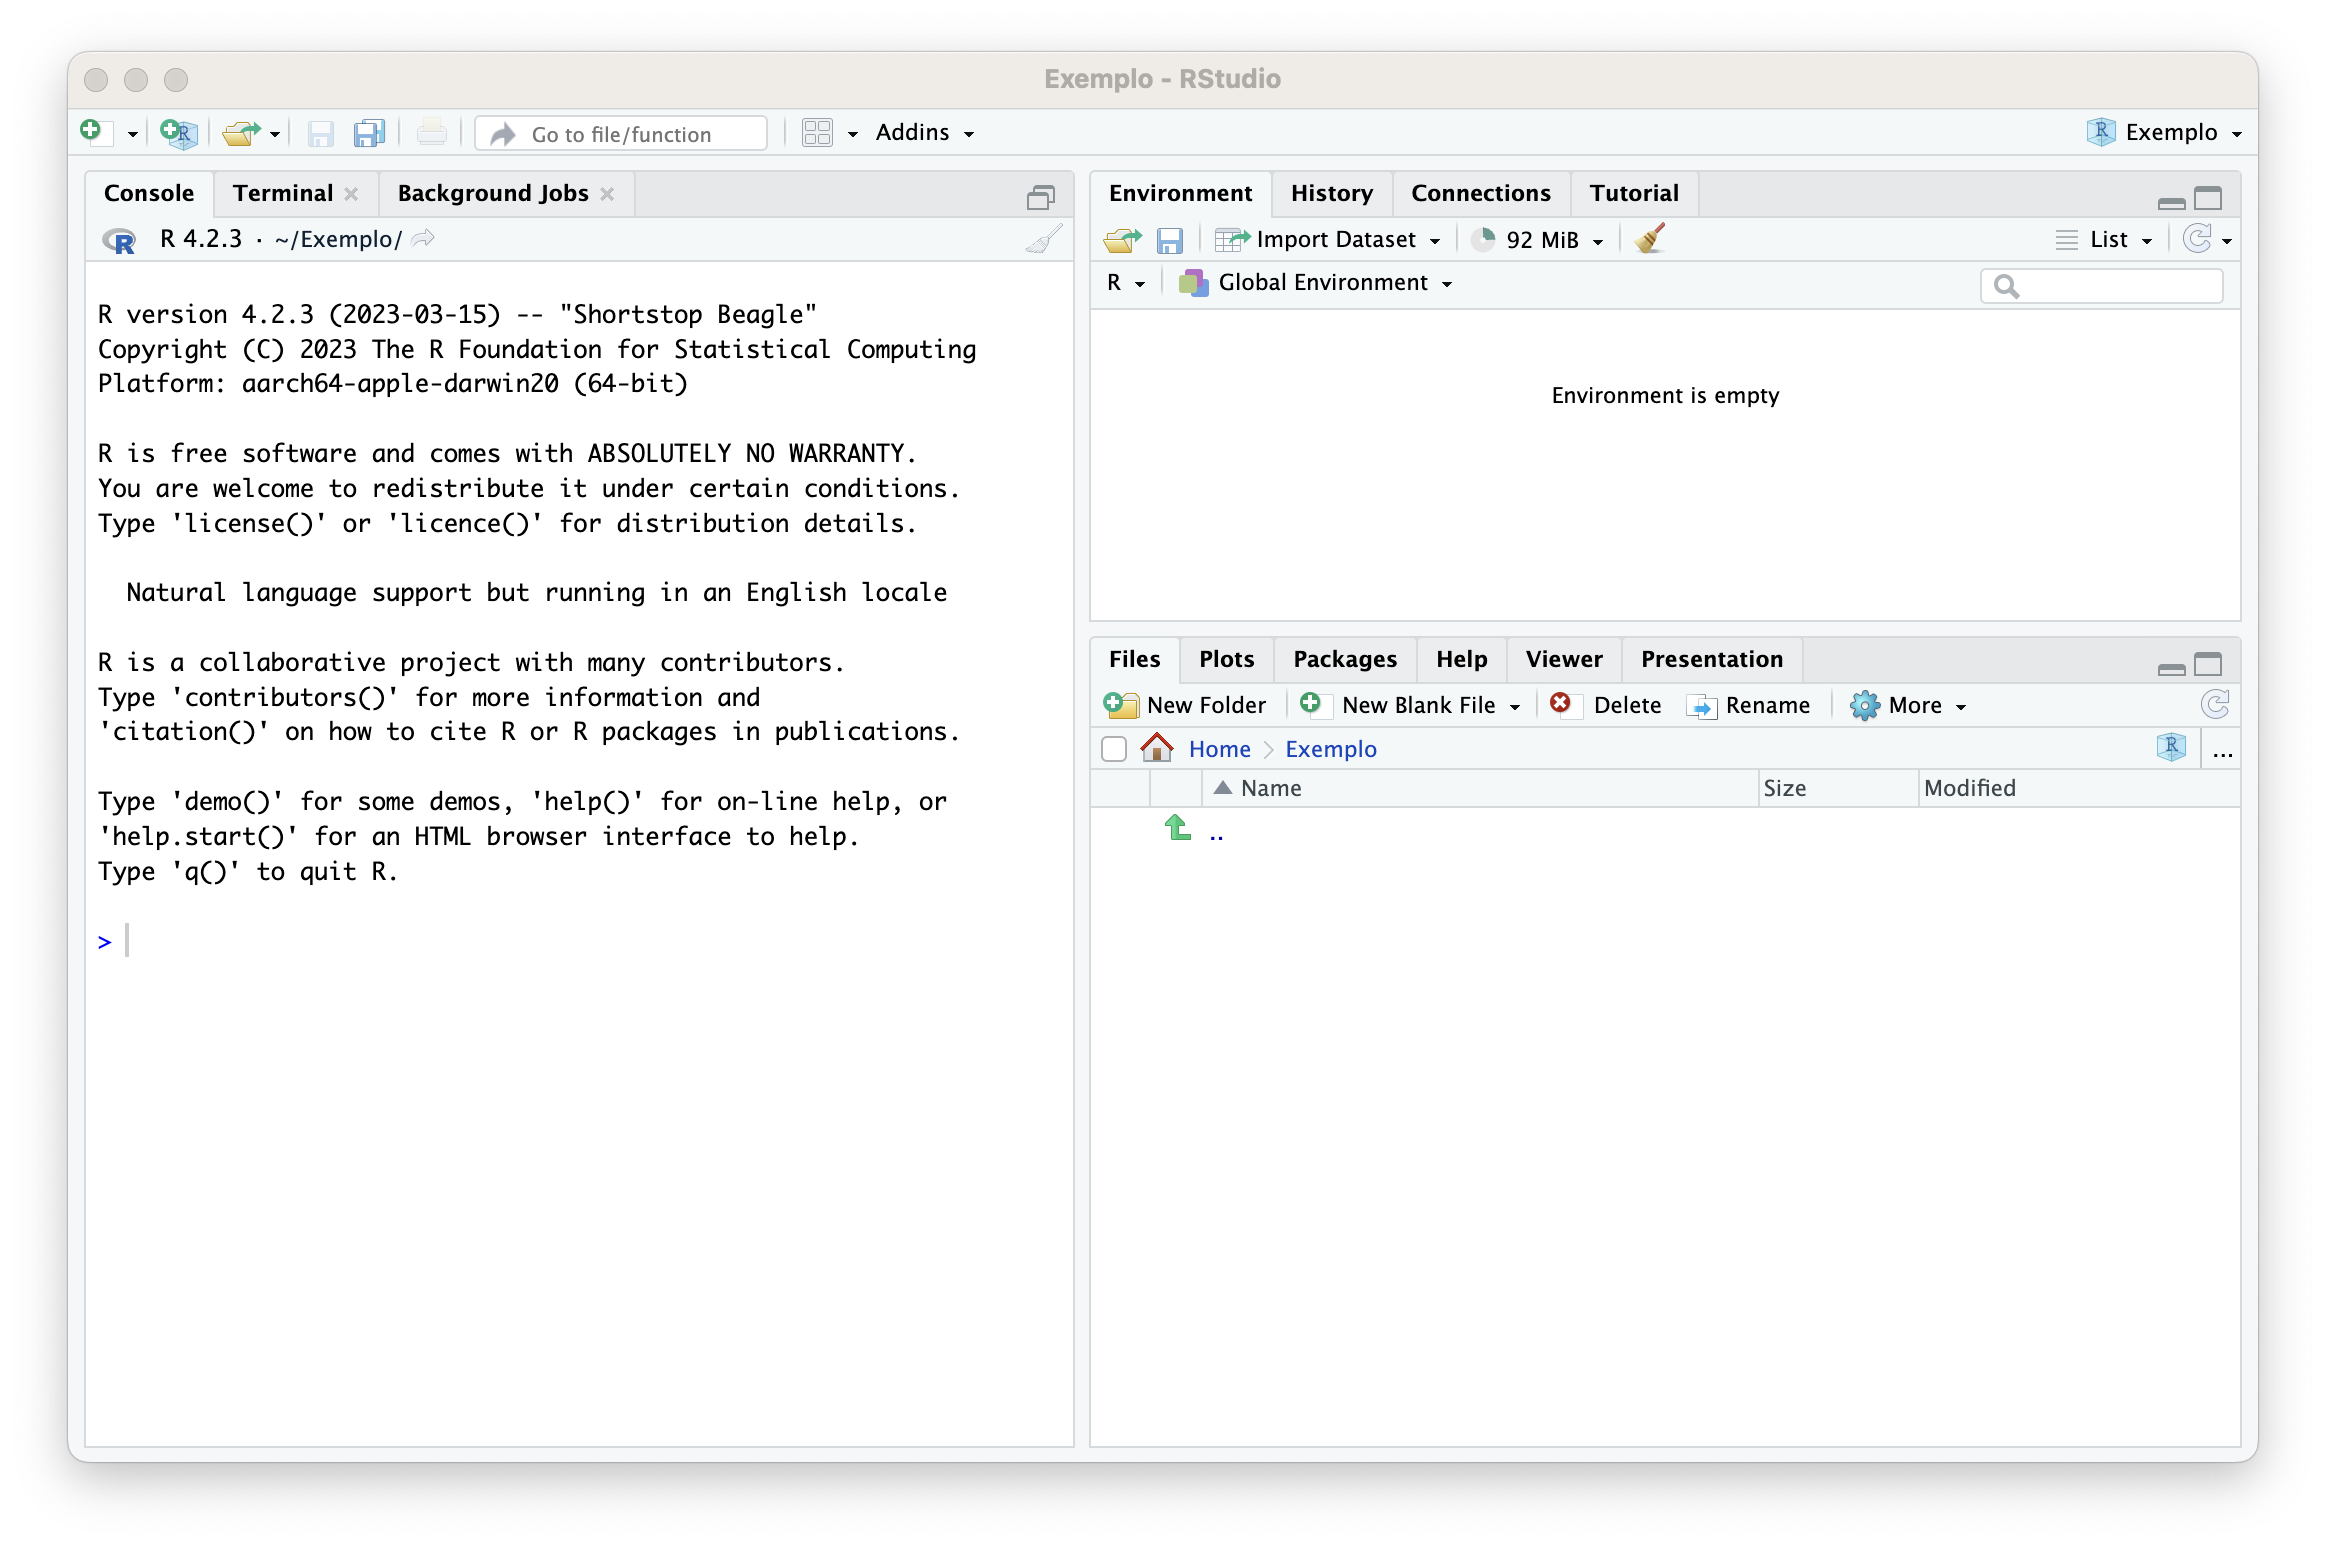
\includegraphics{telaRStudio.png}
\caption{Figura: Tela inicial do RStudio}
\end{figure}

Caso enfrente dificuldades, siga para o Plano B.

\section{Plano B: R e RStudio na Nuvem}\label{plano-b-r-e-rstudio-na-nuvem}

O Plano B é utilizar o RStudio diretamente na nuvem, sem precisar instalar nada. Essa alternativa é excelente, mas requer uma boa conexão com a internet.

Siga os passos:

\begin{enumerate}
\def\labelenumi{\arabic{enumi}.}
\tightlist
\item
  Acesse: \url{https://posit.cloud}
\item
  Faça login (você pode usar sua conta do Google, por exemplo)
\item
  Após o login, você verá esta tela:
\end{enumerate}

\begin{figure}
\centering
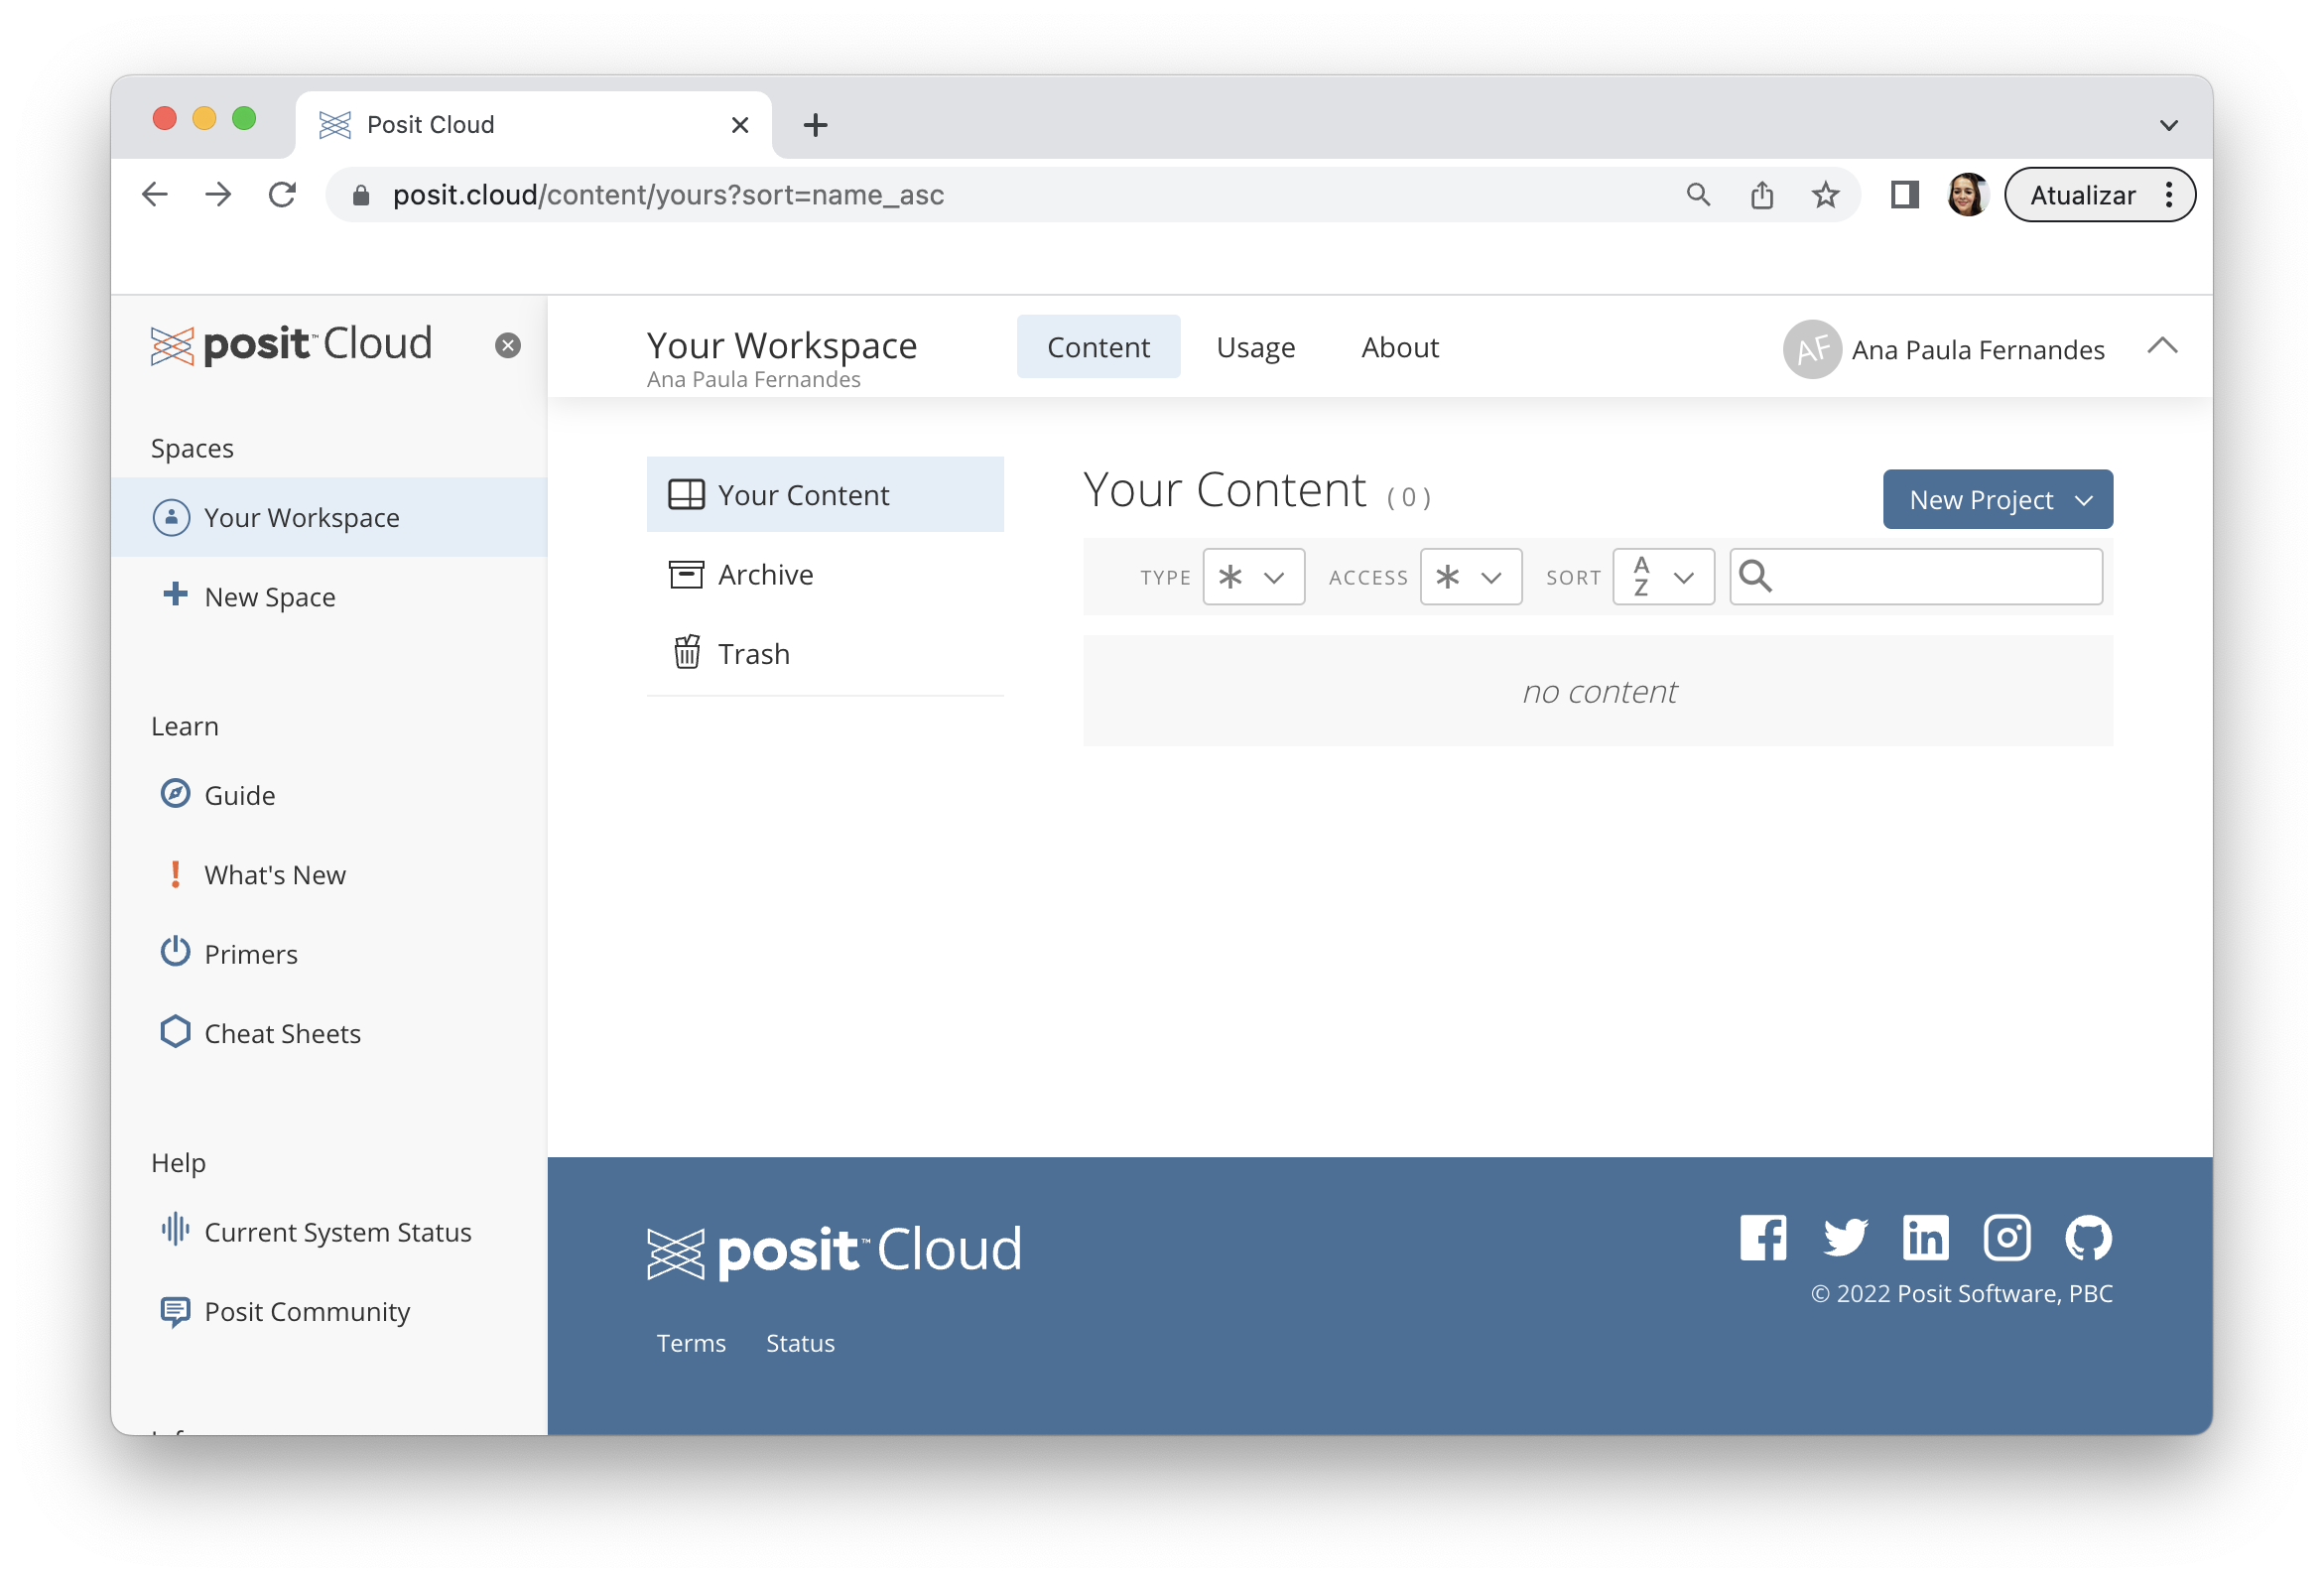
\includegraphics{telaPosit.png}
\caption{Figura: Tela inicial na nuvem da Posit}
\end{figure}

\begin{enumerate}
\def\labelenumi{\arabic{enumi}.}
\setcounter{enumi}{3}
\tightlist
\item
  Crie um novo projeto clicando em \emph{New Project} e, depois, \emph{New RStudio Project}:
\end{enumerate}

\begin{figure}
\centering
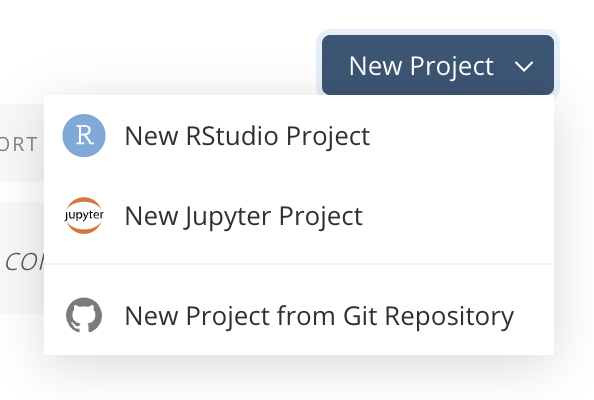
\includegraphics[width=0.4\textwidth,height=\textheight]{telaCriarProjetoRStudio.png}
\caption{Figura: Botão de criação de um novo projeto}
\end{figure}

\begin{enumerate}
\def\labelenumi{\arabic{enumi}.}
\setcounter{enumi}{4}
\tightlist
\item
  Pronto! A interface do RStudio será carregada na nuvem:
\end{enumerate}

\begin{figure}
\centering
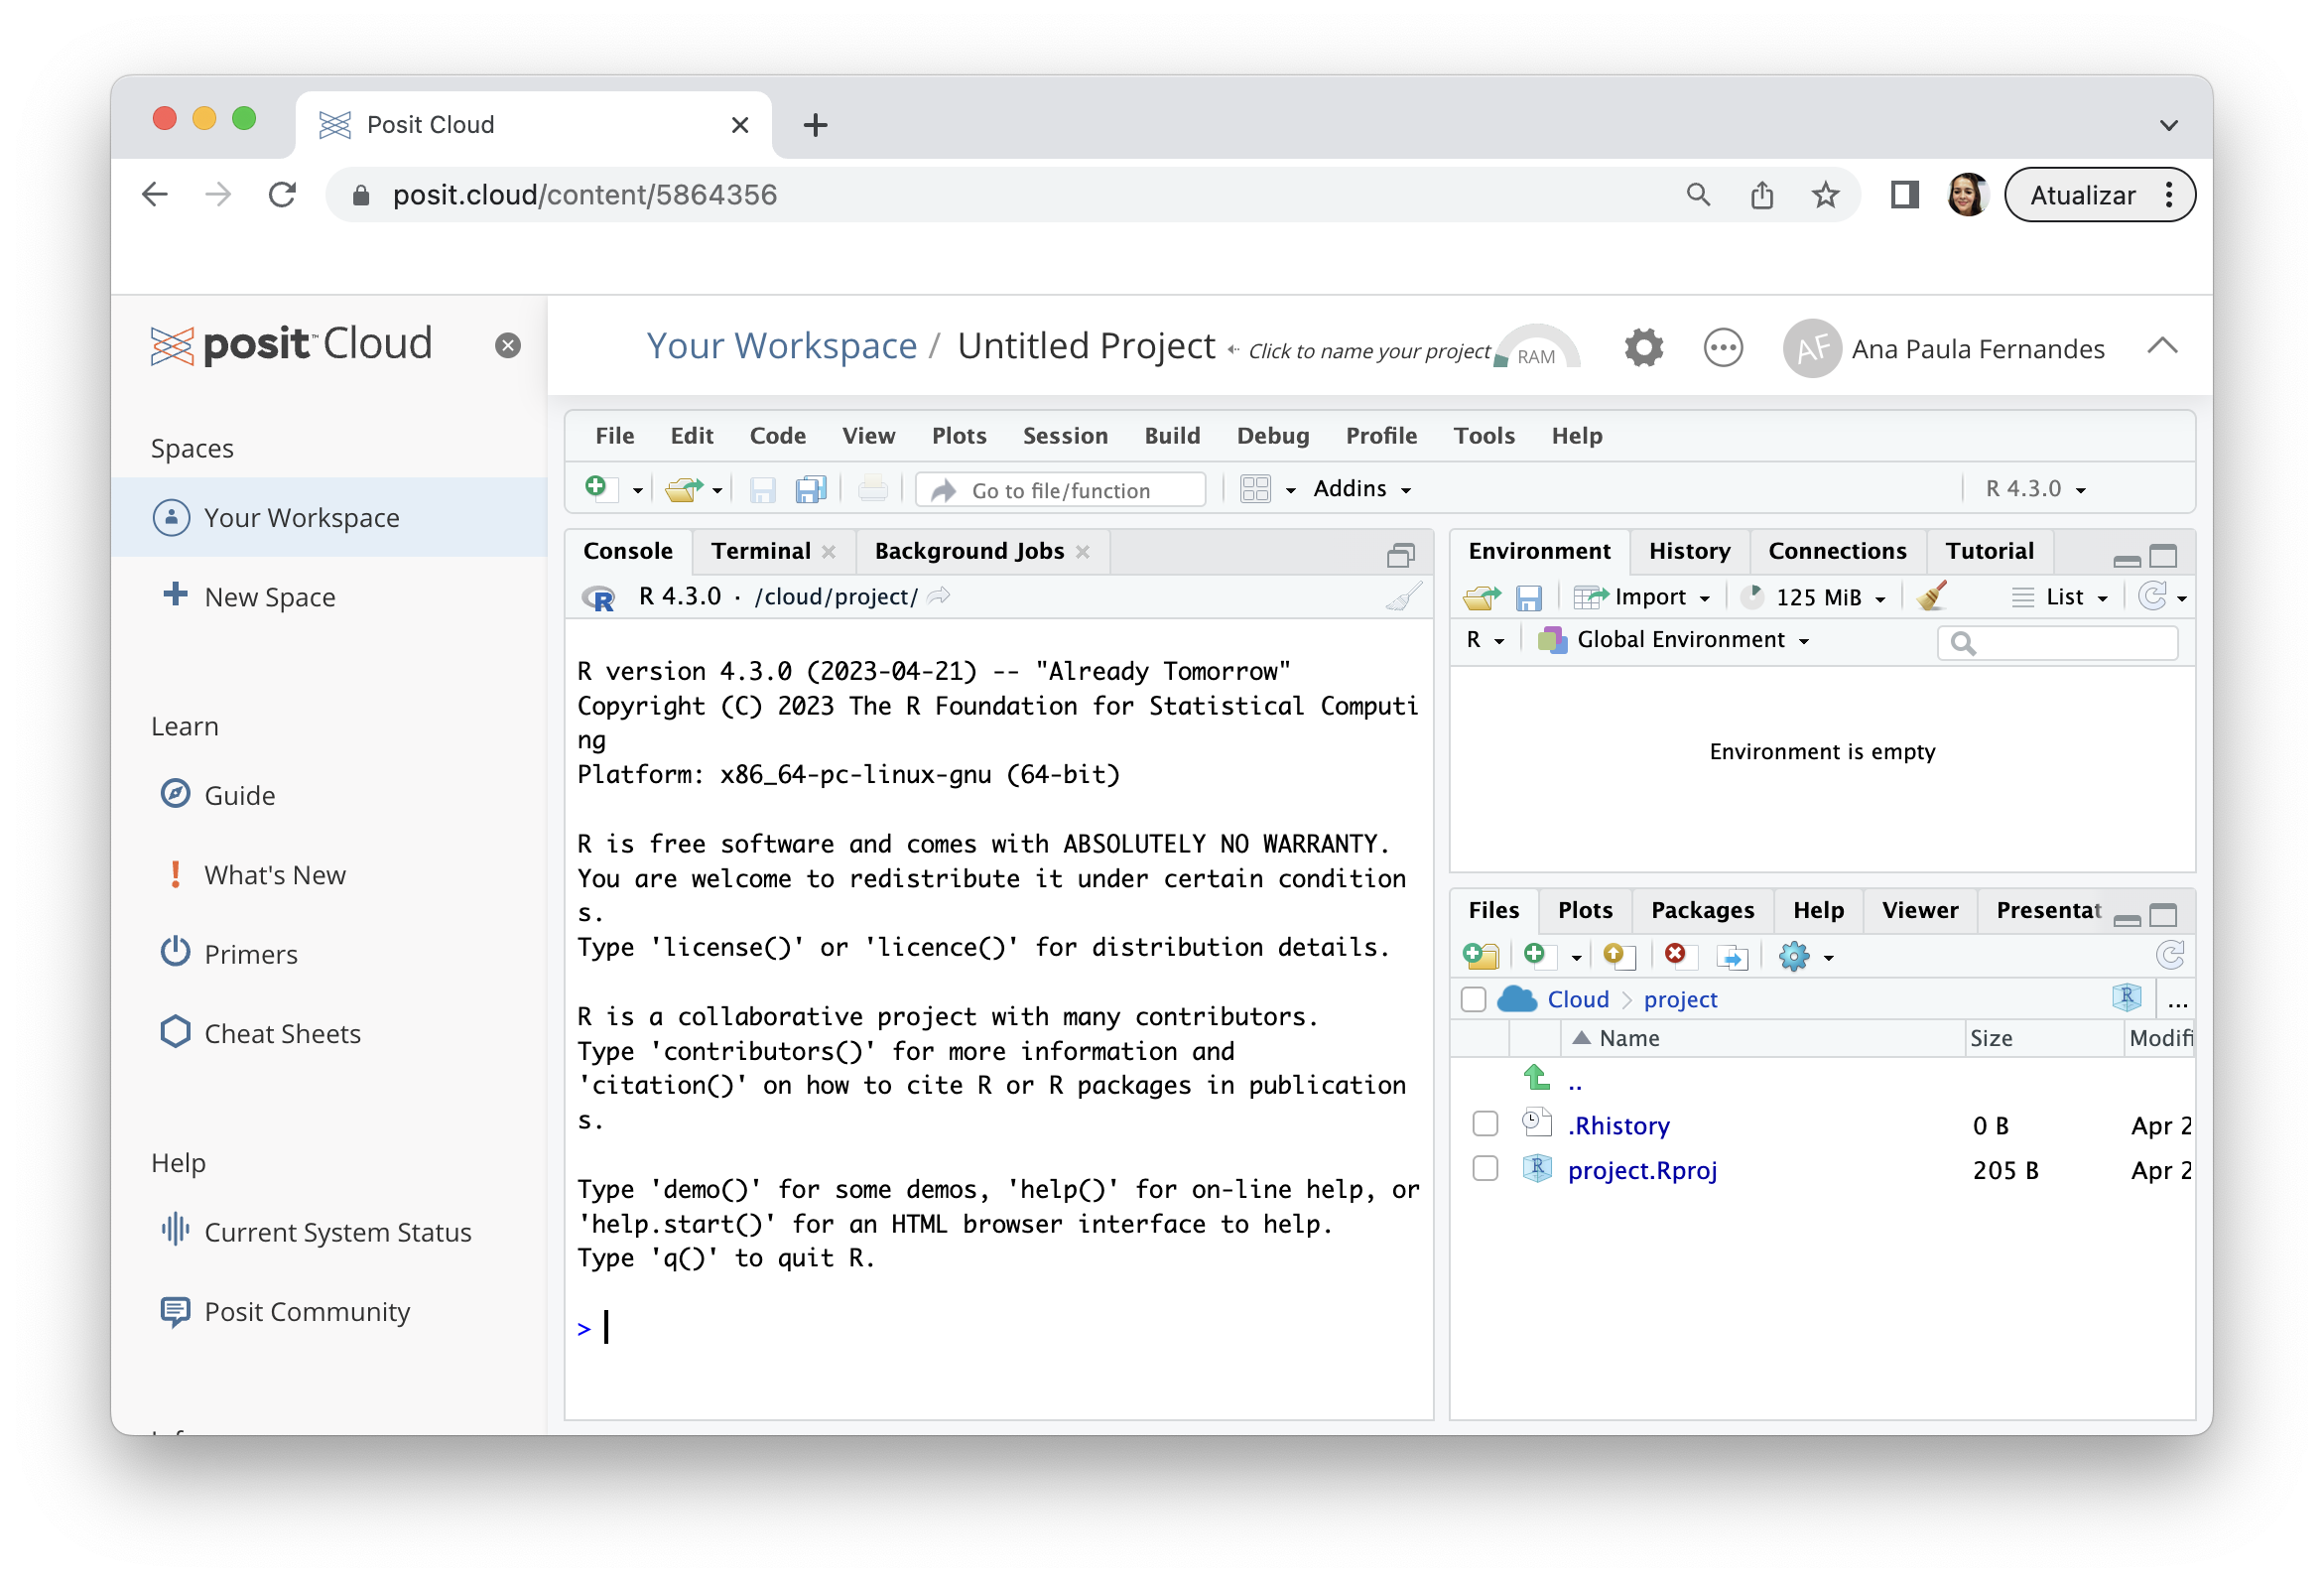
\includegraphics{telaRStudioPosit.png}
\caption{Figura: Tela do RStudio online na Posit Cloud}
\end{figure}

\begin{quote}
Vantagem: seus arquivos e análises ficam salvos na nuvem, em um local seguro e acessível de qualquer lugar.
\end{quote}

\begin{center}\rule{0.5\linewidth}{0.5pt}\end{center}

Com o ambiente configurado, estaremos prontos para explorar o mundo da estatística com R!

\chapter{Trabalhando no RStudio}\label{trabalhando-RStudio}

Seja na versão instalada no seu computador (plano A) ou na nuvem (plano B), conheça melhor as áreas do RStudio:

\begin{enumerate}
\def\labelenumi{\arabic{enumi}.}
\item
  \textbf{Console:} local onde serão apresentadas as respostas para códigos executados;
\item
  \textbf{Ambiente de memória (Environment):} é o cérebro do R, onde ficam registrados os objetos que ele reconhece.
\item
  A área de \textbf{Arquivos (Files), Gráficos (Plots), Pacotes (Packages), Ajuda (Help), Visualização (Viewer) e Apresentação (Presentation)}: mostram, respectivamente, os arquivos do diretório onde estão seus arquivos no computador, os gráficos, os pacotes, a ajuda, a janela de visualização e a apresentação.
\end{enumerate}

A figura abaixo identifica cada uma dessas áreas:

\begin{figure}
\centering
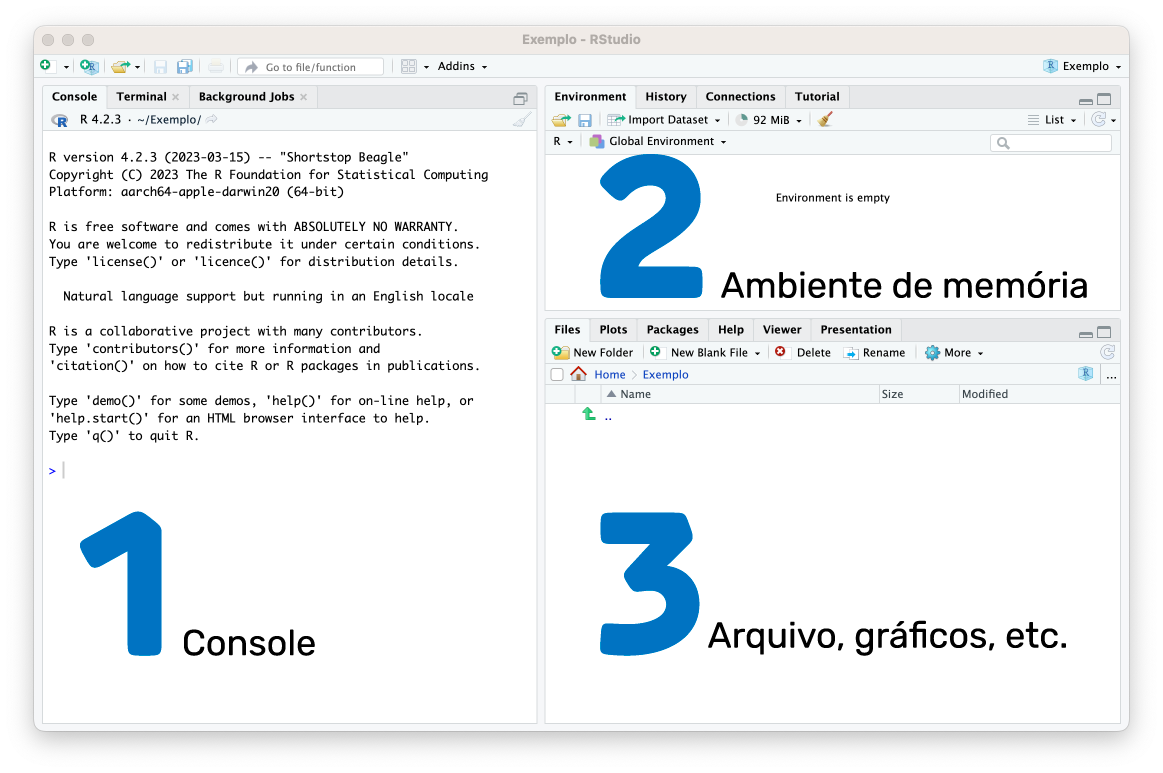
\includegraphics{telaRStudio123.png}
\caption{Figura: Identificação das áreas do RStudio}
\end{figure}

Digitaremos os códigos da linguagem R, em um arquivo que chamamos de \textbf{script}. Para abrir um arquivo do tipo script R, faça:

\begin{enumerate}
\def\labelenumi{\arabic{enumi}.}
\tightlist
\item
  Acesse a opção \textbf{File} no menu principal do RStudio;
\item
  Escolha a opção \textbf{New File};
\item
  E depois a opção \textbf{R Script}.
\end{enumerate}

\begin{figure}
\centering
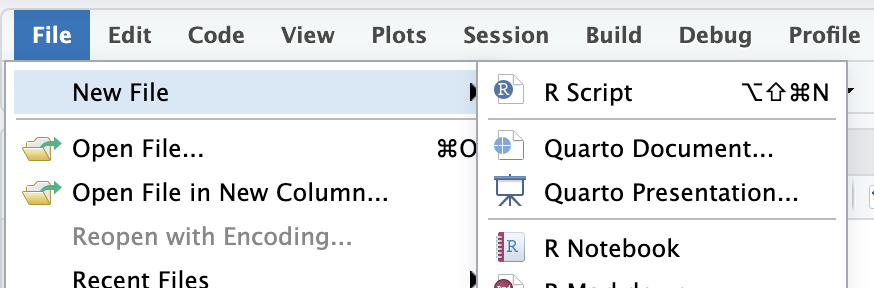
\includegraphics[width=0.4\textwidth,height=\textheight]{arquivoScript.png}
\caption{Figura: Como abrir um novo arquivo de script R}
\end{figure}

Assim, na tela da IDE RStudio aparecerá uma nova área, que é a área do arquivo script, como mostra a figura.

\begin{figure}
\centering
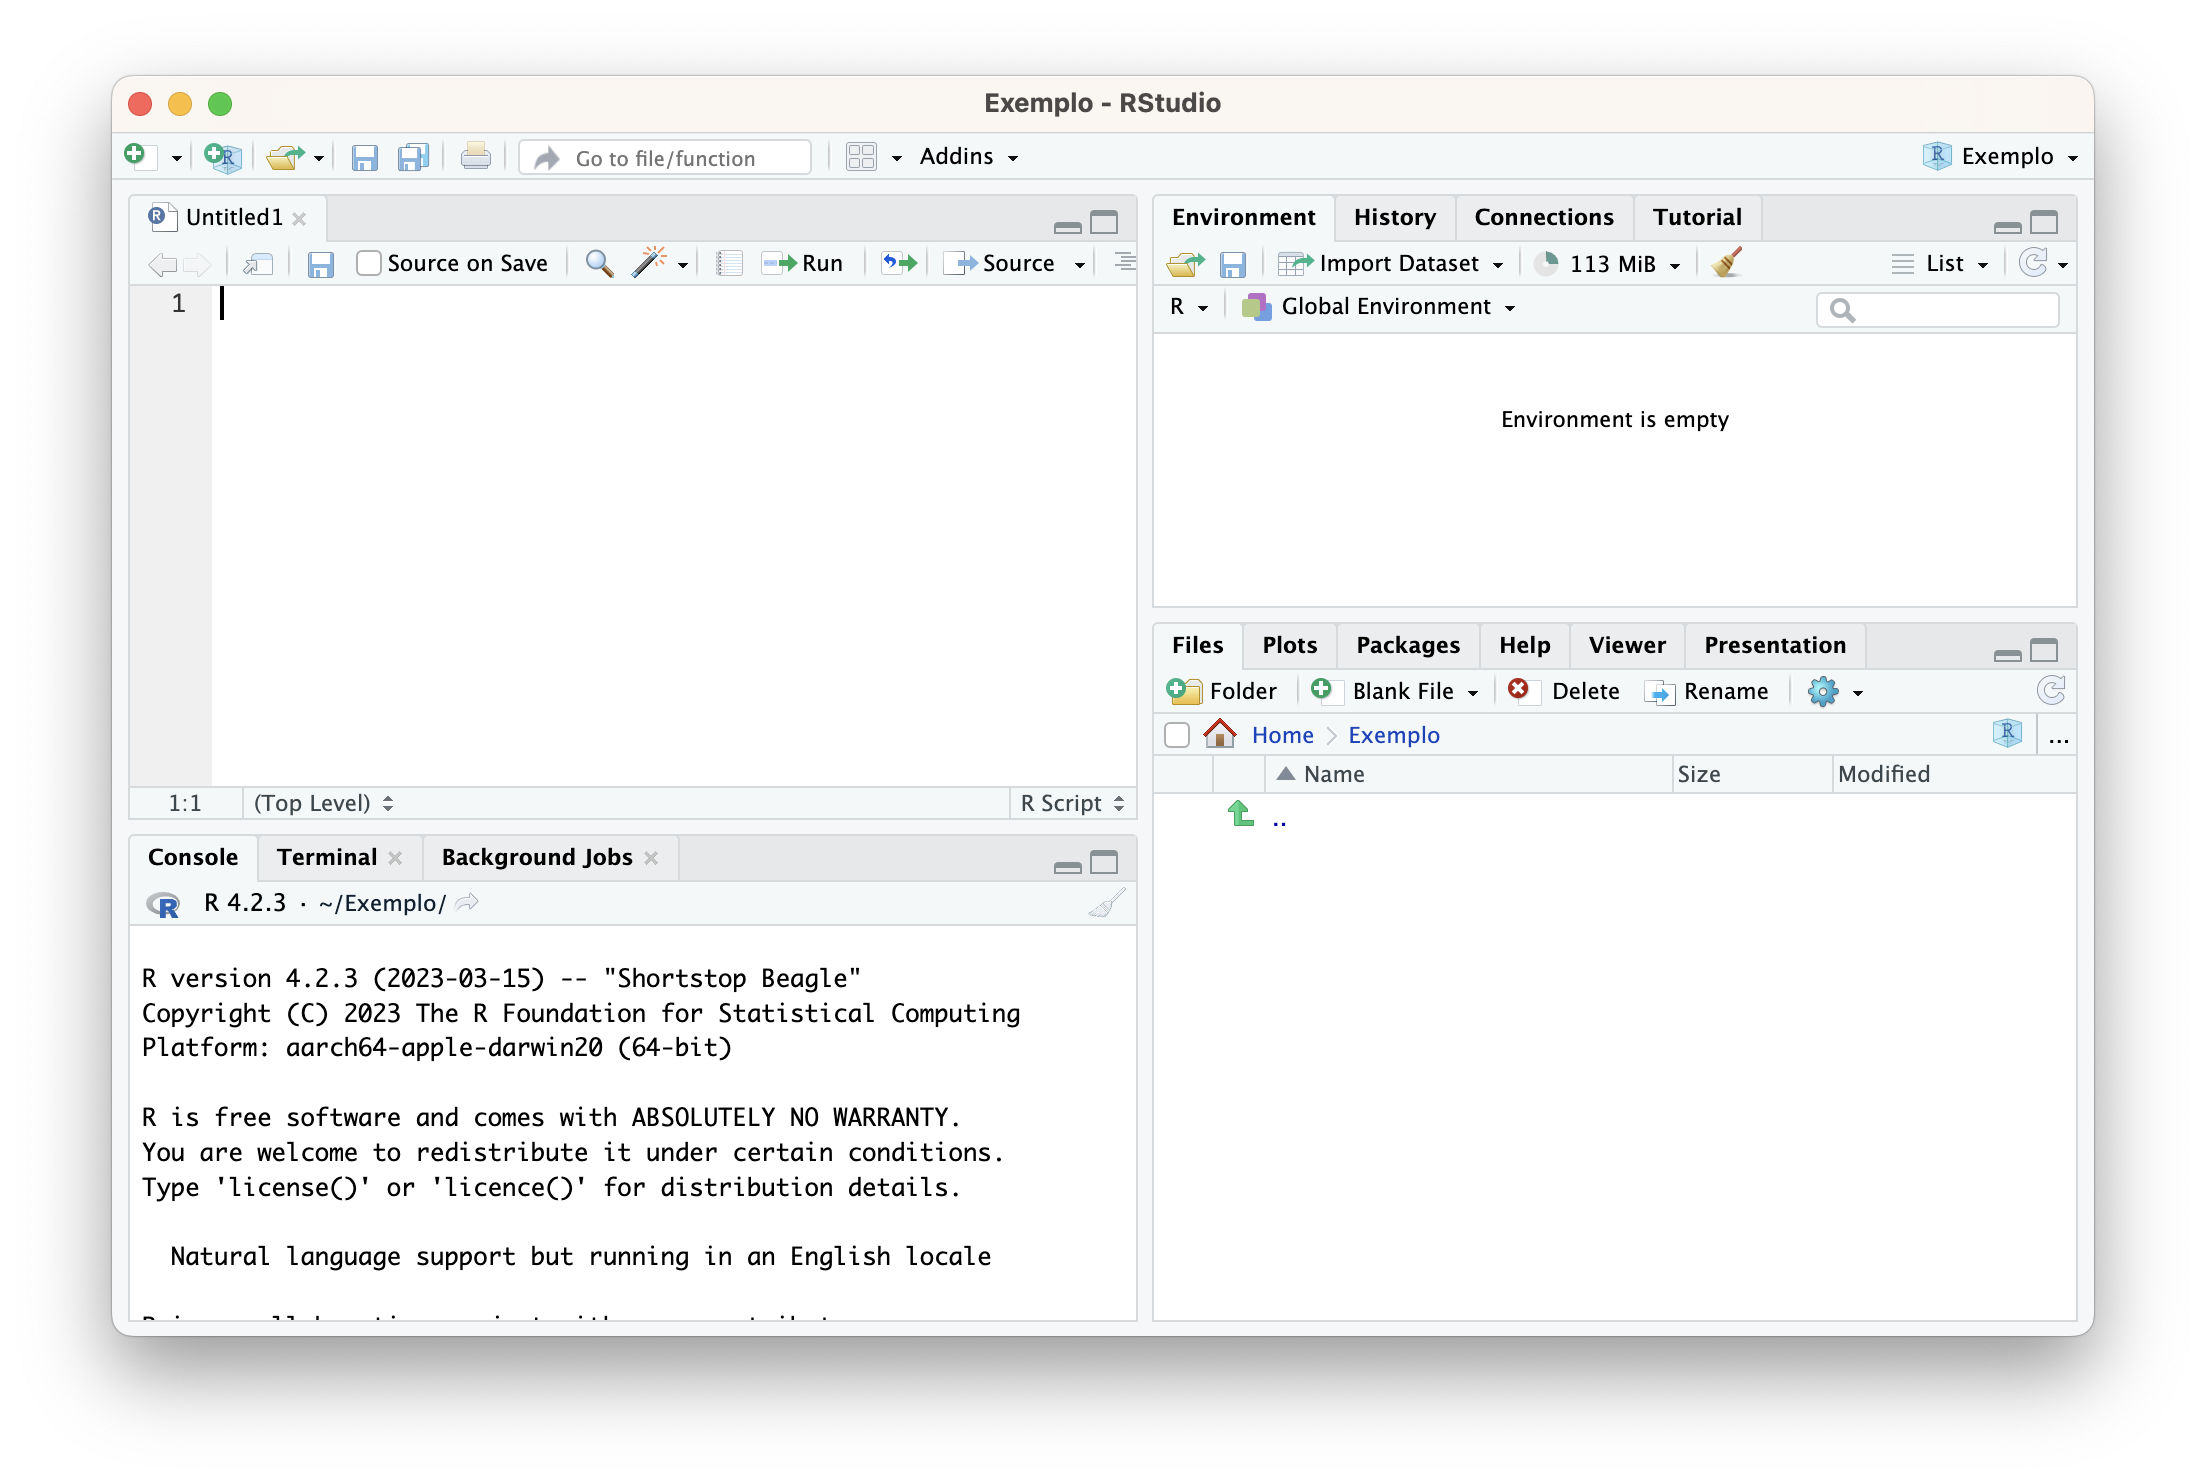
\includegraphics{telaScript.png}
\caption{Figura: Como abrir um novo arquivo de script R}
\end{figure}

Observe que o arquivo está sem um nome (\textbf{Untitled1}, sem título). Salve o arquivo atribuindo-lhe um nome adequado. Para isso, no menu principal, escolha \emph{File}, depois \emph{Save}.

\begin{quote}
Dica: O ideal seria criar um \textbf{Projeto}. Veja a opção \emph{File \textgreater{} New Project}.
\end{quote}

\chapter{Primeiros exercícios no R}\label{primeiros-exercuxedcios-no-r}

Nos capítulos \ref{ambiente-computacional} e \ref{trabalhando-RStudio} vimos sobre o ambiente computacional (computador ou nuvem) e identificamos as 4 áreas da tela da interface do RStudio: \textbf{console}, \textbf{ambiente de memória}, \textbf{arquivos, gráficos, etc.} e \textbf{script}, assim estamos prontos para escrever alguns códigos e executá-los a partir da área de script.

\begin{quote}
\textbf{Atenção:} TODOS os cógigos serão digitados no arquivo de script, seguindo uma sequência lógica de passos, ou seja, escreveremos um roteiro (\emph{script}), como se fosse uma receita de bolo, isso é o que o pessoal da computação chama de algoritmo.
\end{quote}

\section{Exemplo 1}\label{exemplo-1}

\begin{itemize}
\tightlist
\item
  Observe o código escrito na linha 1 do arquivo de script e o botão \textbf{Run} (primeira seta verde):
\end{itemize}

\begin{figure}
\centering
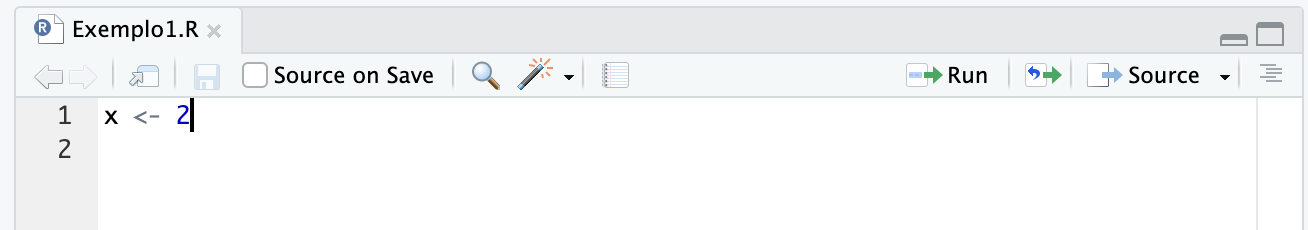
\includegraphics{telaExemplo1.png}
\caption{Figura: Primeiro exemplo de cógigo R}
\end{figure}

\begin{itemize}
\tightlist
\item
  O sequência de caracteres \textbf{\textless-} é o símbolo de atribuição no R.
\end{itemize}

\begin{quote}
Pressionando as teclas ALT e - (menos) simultaneamente cria no script o sinal de atribuição.
\end{quote}

\begin{itemize}
\item
  O código significa que criamos um objeto chamado \textbf{x} e atribuimos a esse objeto o valor 2.
\item
  No entanto, o R ainda não sabe que o valor de x é igual a 2!
\item
  Para registrar essa informação na memória do R, devemos executar essa linha.
\end{itemize}

\begin{quote}
Para executar uma linha posicione o cursor na linha, e clique no botão \textbf{Run}
\end{quote}

\begin{figure}
\centering
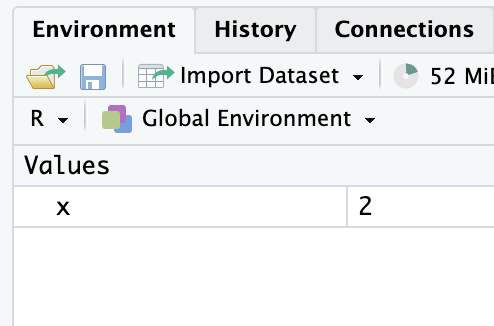
\includegraphics[width=0.4\textwidth,height=\textheight]{telaValorMemoria.png}
\caption{Figura: O objeto x é registrado na memória do R, armazenando o valor igual a 2}
\end{figure}

\begin{quote}
Observe sempre o ambiente de memória (bem como o console) quando executar uma linha.
\end{quote}

\section{Exemplo 2}\label{exemplo-2}

Execute o seguinte cógigo no R.

\begin{Shaded}
\begin{Highlighting}[]
\NormalTok{idades }\OtherTok{\textless{}{-}} \FunctionTok{c}\NormalTok{( }\DecValTok{23}\NormalTok{, }\DecValTok{18}\NormalTok{, }\DecValTok{17}\NormalTok{, }\DecValTok{25}\NormalTok{, }\DecValTok{21}\NormalTok{, }\DecValTok{19}\NormalTok{, }\DecValTok{22}\NormalTok{, }\DecValTok{24}\NormalTok{, }\DecValTok{19}\NormalTok{, }\DecValTok{19}\NormalTok{ )}
\end{Highlighting}
\end{Shaded}

\begin{itemize}
\item
  Esse código significa que foi criado um objeto chamado idade que armazena 10 valores: 23, 18, 17, 25, 21, 19, 22, 24, 19, 19, diferentemente do exemplo 1 em que x armazenava somente o valor 2.
\item
  Isso foi possível pois usamos a função \textbf{c( )}.
\item
  observe que os valores foram colocado dentro dos parênteses da função \textbf{c( )}
\end{itemize}

\begin{quote}
Com função \textbf{c( )} podemos \textbf{combinar} vários valores em um objeto, esse objeto recebe o nome de vetor ou lista.
\end{quote}

\section{Exemplo 3}\label{exemplo-3}

Observe nesse código as funções:

\begin{itemize}
\item
  \textbf{max( )}
\item
  \textbf{min( )}
\item
  \textbf{range( )}
\item
  \textbf{mean( )}
\item
  \textbf{sd( )}
\end{itemize}

\begin{Shaded}
\begin{Highlighting}[]
\CommentTok{\# criando o vetor idades }
\NormalTok{idades }\OtherTok{\textless{}{-}} \FunctionTok{c}\NormalTok{( }\DecValTok{23}\NormalTok{, }\DecValTok{18}\NormalTok{, }\DecValTok{17}\NormalTok{, }\DecValTok{25}\NormalTok{, }\DecValTok{21}\NormalTok{, }\DecValTok{19}\NormalTok{, }\DecValTok{22}\NormalTok{, }\DecValTok{24}\NormalTok{, }\DecValTok{19}\NormalTok{, }\DecValTok{19}\NormalTok{ )}

\CommentTok{\# maior valor}
\CommentTok{\# função max( )}
\FunctionTok{max}\NormalTok{(idades)}
\end{Highlighting}
\end{Shaded}

\begin{verbatim}
## [1] 25
\end{verbatim}

\begin{Shaded}
\begin{Highlighting}[]
\CommentTok{\# menor valor}
\CommentTok{\# função min( )}
\FunctionTok{min}\NormalTok{(idades)}
\end{Highlighting}
\end{Shaded}

\begin{verbatim}
## [1] 17
\end{verbatim}

\begin{Shaded}
\begin{Highlighting}[]
\CommentTok{\# faixa de valores}
\CommentTok{\# função range( )}
\FunctionTok{range}\NormalTok{(idades)}
\end{Highlighting}
\end{Shaded}

\begin{verbatim}
## [1] 17 25
\end{verbatim}

\begin{Shaded}
\begin{Highlighting}[]
\CommentTok{\# média (mean)}
\CommentTok{\# função mean( )}
\FunctionTok{mean}\NormalTok{(idades)}
\end{Highlighting}
\end{Shaded}

\begin{verbatim}
## [1] 20.7
\end{verbatim}

\begin{Shaded}
\begin{Highlighting}[]
\CommentTok{\# desvio padrão (standard deviation)}
\CommentTok{\# função sd() }
\FunctionTok{sd}\NormalTok{(idades)}
\end{Highlighting}
\end{Shaded}

\begin{verbatim}
## [1] 2.710064
\end{verbatim}

\begin{quote}
Copie o código e cole no seu arquivo script, selecione todo conteúdo (CRTL+A) e execute todo o cógigo de uma única vez.
\end{quote}

\begin{itemize}
\tightlist
\item
  Observe que as respostas apareceram no \textbf{console}, conforme mostrado na figura abaixo:
\end{itemize}

\begin{figure}
\centering
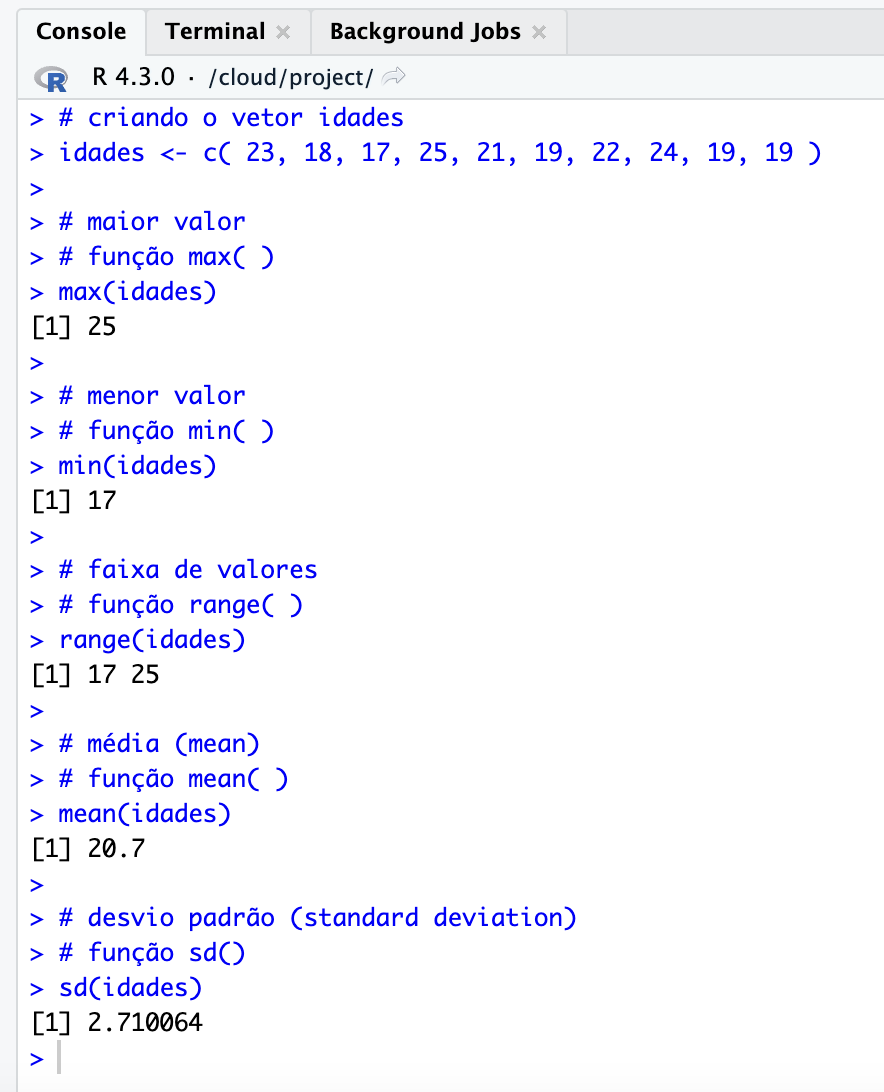
\includegraphics[width=0.4\textwidth,height=\textheight]{telaRespostaConsole.png}
\caption{Figura: Como abrir um novo arquivo de script R}
\end{figure}

\begin{quote}
O símbolo \# é o símbolo de comentário, isso significa que podemos escrever qualquer texto diferente do que o R sabe interpretar, e mesmo executando o código nenhum erro acontece!
\end{quote}

\begin{quote}
\textbf{IMPORTANTE}: é uma boa prática comentar os trechos de códigos para deixar documentado qual é o objetivo do código.
\end{quote}

\chapter{Tipos de Variáveis}\label{tipos-de-variuxe1veis}

As variáveis podem ser classificadas de acordo com sua natureza:

\section{Variáveis Quantitativas}\label{variuxe1veis-quantitativas}

Expressam \textbf{quantidade} e podem ser divididas em:

\begin{itemize}
\tightlist
\item
  \textbf{Discreta}: Assume valores inteiros (contagem).

  \begin{itemize}
  \tightlist
  \item
    \emph{Exemplo}: O número de filhos de uma pessoa. Você pode contar 0, 1, 2, 3 filhos, mas não pode ter 2,5 filhos.
  \end{itemize}
\item
  \textbf{Contínua}: Assume qualquer valor dentro de um intervalo específico (mensuração).

  \begin{itemize}
  \tightlist
  \item
    \emph{Exemplo}: A altura de uma pessoa, que pode ser 1,70 m, 1,71 m, 1,711 m, e assim por diante, com infinitas possibilidades entre os valores.
  \end{itemize}
\end{itemize}

\section{Variáveis Qualitativas}\label{variuxe1veis-qualitativas}

Expressam \textbf{qualidade} e são representadas por \textbf{categorias} ou \textbf{rótulos}. São subdivididas em:

\begin{itemize}
\tightlist
\item
  \textbf{Nominal}: Categorias que não podem ser ordenadas.

  \begin{itemize}
  \tightlist
  \item
    \emph{Exemplo}: O tipo de fruta que você prefere, como maçã, banana, laranja. Não faz sentido ordenar essas categorias de maneira que uma seja ``maior'' que a outra.
  \end{itemize}
\item
  \textbf{Ordinal}: Categorias que podem ser ordenadas, com uma graduação entre elas.

  \begin{itemize}
  \tightlist
  \item
    \emph{Exemplo}: Níveis de satisfação de um serviço, como ``satisfeito'', ``neutro'' e ``insatisfeito''. Aqui, existe uma ordem em que ``satisfeito'' é maior que ``neutro'', e ``neutro'' é maior que ``insatisfeito''.
  \end{itemize}
\end{itemize}

Uma aplicação comum das variáveis ordinais é a \textbf{Escala Likert}, que é amplamente utilizada em pesquisas de opinião para medir atitudes ou percepções. A escala Likert geralmente apresenta uma série de afirmativas, e o participante deve indicar seu nível de concordância com cada uma delas, com respostas em uma sequência ordenada.

\emph{Exemplo}: Em uma pesquisa de satisfação de clientes, a pergunta poderia ser: ``Concordo que a alimentação oferecida pelo hospital foi satisfatória.'' As opções de resposta poderiam ser:

\begin{enumerate}
\def\labelenumi{\arabic{enumi}.}
\tightlist
\item
  \textbf{Discordo totalmente}
\item
  \textbf{Discordo parcialmente}
\item
  \textbf{Neutro}
\item
  \textbf{Concordo parcialmente}
\item
  \textbf{Concordo totalmente}
\end{enumerate}

Essas respostas formam uma escala ordinal, pois a ordem das categorias reflete um aumento no nível de concordância, mas as diferenças entre elas não são necessariamente iguais.

\begin{quote}
\textbf{Dica}: Veja o vídeo do Prof.~Heitor no \textbf{Canal Pesquise}: \href{https://youtu.be/_oc37Ea_tl8}{Assista aqui}.
\end{quote}

\section{Aplicação das Variáveis em Estatística}\label{aplicauxe7uxe3o-das-variuxe1veis-em-estatuxedstica}

A natureza da variável influencia o tipo de procedimento estatístico que será utilizado. Exemplos:

\subsection{Estatística Descritiva:}\label{estatuxedstica-descritiva-1}

\begin{itemize}
\tightlist
\item
  \textbf{Variáveis Qualitativas}: São representadas por sua \textbf{frequência absoluta} ou \textbf{percentual}.

  \begin{itemize}
  \tightlist
  \item
    \emph{Exemplo}: Em uma pesquisa de preferência de frutas, pode-se dizer que 40\% das pessoas escolheram maçã, 35\% escolheram banana, e 25\% escolheram laranja.
  \end{itemize}
\item
  \textbf{Variáveis Quantitativas}: São representadas por \textbf{medidas resumo}, como \textbf{média} e \textbf{desvio padrão}.

  \begin{itemize}
  \tightlist
  \item
    \emph{Exemplo}: Se você calcular a média de altura de um grupo de pessoas, e o desvio padrão indicar que a altura das pessoas varia em torno de 5 cm da média.
  \end{itemize}
\end{itemize}

\subsection{Estatística Inferencial:}\label{estatuxedstica-inferencial-1}

\begin{itemize}
\tightlist
\item
  \textbf{Teste Qui-Quadrado}: Usado para verificar se há associação entre as categorias de duas variáveis qualitativas.

  \begin{itemize}
  \tightlist
  \item
    \emph{Exemplo}: Um teste Qui-Quadrado poderia ser utilizado para verificar se a escolha de fruta (maçã, banana, laranja) tem relação com o sexo (masculino, feminino) dos participantes.
  \end{itemize}
\item
  \textbf{Teste de Correlação de Pearson}: Mede a força da correlação linear entre duas variáveis quantitativas.

  \begin{itemize}
  \tightlist
  \item
    \emph{Exemplo}: O teste de Pearson poderia ser utilizado para verificar se existe uma relação entre a altura e o peso das pessoas. Quanto maior a altura, maior o peso? Esse teste nos diria a força dessa relação.
  \end{itemize}
\end{itemize}

\section{Atividade 3}\label{atividade-3}

\textbf{Leia o artigo \emph{Estado nutricional, tempo de internação e mortalidade em pacientes submetidos à cirurgia cardíaca em um hospital na cidade de Maceió}}\\
Disponível em: \href{https://www.rasbran.com.br/rasbran/article/view/1724/443}{RASBRAN, Revista da Associação Brasileira de Nutrição, 2023}\\
Acesse também o portal: \href{https://www.rasbran.com.br/}{RASBRAN - Revista da Associação Brasileira de Nutrição}.

\subsection{Análise das Tabelas}\label{anuxe1lise-das-tabelas}

\begin{itemize}
\tightlist
\item
  \textbf{Tabela 1 - Características clínicas dos pacientes submetidos à cirurgia cardíaca}: Esta tabela apresenta as características da amostra analisada na pesquisa.

  \begin{itemize}
  \tightlist
  \item
    \textbf{Tarefa}: Classifique as variáveis (características) em \textbf{qualitativas} e \textbf{quantitativas}.
  \item
    \textbf{Observação}: Verifique como as variáveis foram resumidas. Elas foram apresentadas em \textbf{porcentagens}? Ou foram calculadas medidas de \textbf{média} e \textbf{desvio padrão}?
  \end{itemize}
\item
  \textbf{Tabela 2 - Associação entre estado nutricional, sexo, idade e tempo de internação hospitalar entre os pacientes submetidos à cirurgia cardíaca}\\
\item
  \textbf{Tabela 3 - Associação entre evolução clínica, sexo, idade, tempo de internação hospitalar e estado nutricional entre os pacientes submetidos à cirurgia cardíaca}: Estas tabelas mostram os resultados de um \textbf{teste de hipótese} (parte da estatística inferencial).

  \begin{itemize}
  \tightlist
  \item
    \textbf{Tarefa}: Identifique qual \textbf{teste estatístico} foi aplicado.
  \item
    \textbf{Objetivo}: Qual é o objetivo deste teste?
  \end{itemize}
\end{itemize}

\chapter{Estatística Descritiva}\label{estatuxedstica-descritiva-2}

A estatística descritiva permite \textbf{resumir, organizar e interpretar} dados de forma clara e objetiva. Para isso, utilizamos \textbf{medidas de tendência central}, \textbf{medidas de dispersão} e \textbf{medidas relativas de variabilidade}.

\section{Medidas de Tendência Central (ou Posição)}\label{medidas-de-tenduxeancia-central-ou-posiuxe7uxe3o}

\subsection{Média}\label{muxe9dia}

\begin{itemize}
\tightlist
\item
  \textbf{Definição:} Soma de todos os valores dividida pelo número de observações.\\
\item
  \textbf{Interpretação:} Representa o valor médio ou típico do conjunto de dados.\\
\item
  \textbf{Como reportar:}
\end{itemize}

\begin{quote}
A média dos batimentos cardíacos foi de 58,6 bpm, indicando o valor médio da amostra analisada.
\end{quote}

\subsection{Mediana}\label{mediana}

\begin{itemize}
\tightlist
\item
  \textbf{Definição:} Valor central de um conjunto ordenado de dados.\\
\item
  \textbf{Interpretação:} Divide o conjunto de dados ao meio, sendo útil quando há valores extremos (outliers).\\
\item
  \textbf{Como reportar:}
\end{itemize}

\begin{quote}
A mediana dos batimentos foi de 60,0 bpm, indicando que 50\% dos indivíduos apresentaram valores abaixo ou iguais a esse valor.
\end{quote}

\subsection{Quartis}\label{quartis}

\begin{itemize}
\tightlist
\item
  \textbf{Definição:} Q1 (primeiro quartil) e Q3 (terceiro quartil) representam os valores que dividem os 25\% e os 75\% inferiores dos dados, respectivamente.\\
\item
  \textbf{Interpretação:} Ajudam a entender a distribuição dos dados e identificar a dispersão em torno da mediana.\\
\item
  \textbf{Como reportar:}
\end{itemize}

\begin{quote}
O primeiro e o terceiro quartis foram 54,0 bpm e 64,0 bpm, respectivamente, revelando que 50\% dos batimentos ficaram entre esses dois valores.
\end{quote}

\subsection{Moda}\label{moda}

\begin{itemize}
\tightlist
\item
  \textbf{Definição:} Valor mais frequente do conjunto de dados.\\
\item
  \textbf{Interpretação:} Indica o valor mais comum, embora possa não existir ou haver mais de uma moda.\\
\item
  \textbf{Como reportar:}
\end{itemize}

\begin{quote}
A moda foi 62 bpm, valor que ocorreu com maior frequência na amostra.
\end{quote}

\textbf{Observação importante:}\\
- \textbf{Média e desvio padrão} são medidas que devem ser usadas juntas, especialmente para dados simétricos (distribuição simétrica) e sem valores extremos.
- \textbf{Mediana e quartis} formam outro conjunto de medidas, mais apropriado quando há assimetria ou presença de outliers.

\textbf{Sugestão de vídeo:} Canal Pesquise - \href{https://youtu.be/ot0aDB-grDY}{Tendência Central}

\section{Medidas de Dispersão (ou Variabilidade)}\label{medidas-de-dispersuxe3o-ou-variabilidade}

\subsection{Amplitude}\label{amplitude}

\begin{itemize}
\tightlist
\item
  \textbf{Definição:} Diferença entre o maior e o menor valor.\\
\item
  \textbf{Interpretação:} Indica o intervalo total em que os dados variam.\\
\item
  \textbf{Como reportar:}
\end{itemize}

\begin{quote}
A amplitude foi de 36 bpm, com valores variando de 39 a 75 bpm.
\end{quote}

\subsection{Variância}\label{variuxe2ncia}

\begin{itemize}
\tightlist
\item
  \textbf{Definição:} Média dos quadrados das diferenças entre os valores e a média.\\
\item
  \textbf{Interpretação:} Mede a dispersão, mas sua unidade é o quadrado da unidade original.\\
\item
  \textbf{Como reportar:}
\end{itemize}

\begin{quote}
A variância foi de 98,8 bpm², indicando a variabilidade dos batimentos em relação à média.
\end{quote}

\textbf{Observação:}\\
A unidade da variância é expressa ao quadrado da unidade original dos dados (por exemplo, bpm² no caso de batimentos por minuto), o que pode dificultar sua interpretação direta.\\
Por isso, costuma-se utilizar o \textbf{desvio padrão}, que tem a \textbf{mesma unidade dos dados originais} e fornece uma noção mais intuitiva da dispersão dos valores em torno da média.

\subsection{Desvio padrão (DP)}\label{desvio-padruxe3o-dp}

\begin{itemize}
\tightlist
\item
  \textbf{Definição:} Raiz quadrada da variância.\\
\item
  \textbf{Interpretação:} Expressa, em média, o quanto os dados se afastam da média.\\
\item
  \textbf{Como reportar:}
\end{itemize}

\textbf{Como reportar:}\\
O desvio padrão foi de 9,9 bpm, o que indica que, em média, os batimentos cardíacos dos indivíduos da amostra variam aproximadamente 9,9 unidades em relação à média.

\subsection{Amplitude interquartil (IQR)}\label{amplitude-interquartil-iqr}

\begin{itemize}
\tightlist
\item
  \textbf{Definição:} Diferença entre o terceiro e o primeiro quartis (Q3 - Q1).\\
\item
  \textbf{Interpretação:} Indica a dispersão dos 50\% centrais dos dados.\\
\item
  \textbf{Como reportar:}
\end{itemize}

\begin{quote}
A amplitude interquartil foi de 10,0 bpm, mostrando a concentração dos valores médios.
\end{quote}

\textbf{Sugestão de vídeo:} Canal Pesquise - \href{https://youtu.be/sISPcOIcwXs}{Variabilidade}

\section{Medida Relativa de Variabilidade}\label{medida-relativa-de-variabilidade}

\subsection{Coeficiente de Variação (CV)}\label{coeficiente-de-variauxe7uxe3o-cv}

\begin{itemize}
\tightlist
\item
  \textbf{Definição:} Quociente entre o desvio padrão e a média, multiplicado por 100.\\
\item
  \textbf{Interpretação:} Expressa a variabilidade dos dados em relação à média, permitindo comparar conjuntos com unidades diferentes.\\
\item
  \textbf{Como reportar:}
\end{itemize}

\begin{quote}
O coeficiente de variação foi de 16,9\%, indicando que os dados são relativamente homogêneos.
\end{quote}

\textbf{Observação:}\\
Um CV inferior a 25\% geralmente indica homogeneidade; valores muito altos indicam alta variabilidade.

\section{Funções no R}\label{funuxe7uxf5es-no-r}

Com um vetor \texttt{x} contendo os dados, utilize:

\begin{longtable}[]{@{}ll@{}}
\toprule\noalign{}
Medida & Código R \\
\midrule\noalign{}
\endhead
\bottomrule\noalign{}
\endlastfoot
Média & \texttt{mean(x)} \\
Mediana & \texttt{median(x)} \\
Primeiro quartil (Q1) & \texttt{quantile(x,\ 0.25)} \\
Terceiro quartil (Q3) & \texttt{quantile(x,\ 0.75)} \\
Moda & \texttt{sort(table(x))} \\
Menor valor & \texttt{min(x)} \\
Maior valor & \texttt{max(x)} \\
Resumo geral & \texttt{summary(x)} \\
Amplitude & \texttt{range(x)} \\
Variância & \texttt{var(x)} \\
Desvio padrão & \texttt{sd(x)} \\
Amplitude interquartil & \texttt{IQR(x)} \\
Coeficiente de variação & \texttt{sd(x)/mean(x)*100} \\
\end{longtable}

\begin{quote}
Calcular é importante, mas interpretar corretamente é essencial. Ao elaborar suas interpretações, descreva o que os números revelam sobre o fenômeno analisado.
\end{quote}

\section{Atividade 4}\label{atividade-4}

\textbf{Considere o objeto Batimentos, que é uma amostra de batimentos cardíacos de 20 homens.}

\begin{Shaded}
\begin{Highlighting}[]
\NormalTok{Batimentos }\OtherTok{\textless{}{-}} \FunctionTok{c}\NormalTok{(}\DecValTok{62}\NormalTok{, }\DecValTok{55}\NormalTok{, }\DecValTok{56}\NormalTok{, }\DecValTok{46}\NormalTok{, }\DecValTok{75}\NormalTok{, }\DecValTok{67}\NormalTok{, }\DecValTok{62}\NormalTok{, }\DecValTok{75}\NormalTok{, }\DecValTok{60}\NormalTok{, }\DecValTok{54}\NormalTok{, }\DecValTok{69}\NormalTok{, }\DecValTok{63}\NormalTok{, }\DecValTok{39}\NormalTok{, }\DecValTok{57}\NormalTok{, }\DecValTok{40}\NormalTok{, }\DecValTok{39}\NormalTok{, }\DecValTok{64}\NormalTok{, }\DecValTok{71}\NormalTok{, }\DecValTok{61}\NormalTok{, }\DecValTok{54}\NormalTok{)}
\end{Highlighting}
\end{Shaded}

\begin{itemize}
\tightlist
\item
  Obtenha as seguintes medidas:

  \begin{itemize}
  \tightlist
  \item
    Menor valor:
  \item
    Maior valor:
  \item
    Média:
  \item
    Mediana:
  \item
    Primeiro quartil:
  \item
    Terceiro quartil:
  \item
    Variância:
  \item
    Desvio padrão:
  \item
    Amplitude interquartil:
  \item
    Coeficiente de varição:
  \end{itemize}
\item
  Escreva sobre o conjunto media e desvio padrão:
\end{itemize}

\begin{quote}
A média dos dados foi de X (unidade), com um desvio padrão de Y (unidade), indicando que os valores estão, em geral, relativamente próximos/espalhados em torno da média. O desvio padrão reflete a quantidade de variabilidade ou dispersão dos dados em relação à média, e neste caso, a dispersão é baixa/média/alta, dependendo do valor de Y.
\end{quote}

\begin{itemize}
\tightlist
\item
  Escreva sobre conjunto mediana e quartis:
\end{itemize}

\begin{quote}
A mediana foi Z (unidade), e o intervalo interquartil (IQR), que representa a diferença entre o terceiro quartil (Q3) e o primeiro quartil (Q1), foi Q3 - Q1 (unidade). Isso indica que 50\% dos dados estão concentrados nesse intervalo.
\end{quote}

\begin{itemize}
\tightlist
\item
  Escreva sobre o coeficiente de variação:
\end{itemize}

\begin{quote}
O coeficiente de variação (CV) foi calculado como X\%, o que reflete a dispersão relativa dos dados em relação à média. Valores mais baixos de CV indicam que os dados estão mais concentrados em torno da média, enquanto valores mais altos indicam uma maior dispersão.
\end{quote}

\begin{itemize}
\tightlist
\item
  Acrescente mais uma amostra com valor de batimento igual a 120, recalcule as medidas acima. Qual conjunto você consideraria mais adequado para resumir sua amostra, na presença desse valor discrepante (\emph{outlier})? A média (DP) ou mediana (1o.Q ; 3o.Q)? Explique.
\end{itemize}

\chapter{Importando banco de dados}\label{importando-banco-de-dados}

Na prática, os dados que vamos analisar estarão armazenado em um \textbf{banco de dados}, um arquivo de banco de dados pode ser de diferentes tipos, por exemplo:

\begin{itemize}
\item
  Arquivo do tipo Excel (xls ou xlsx)
\item
  Arquivo de texto separado por vírgulas (csv - \emph{comma-separated values})
\end{itemize}

\begin{quote}
Existem várias fontes de dados abertas, onde podemos baixar um banco de dados para realizar analises estatísticas, aqui estão algumas delas:
\end{quote}

\begin{itemize}
\item
  DataSus: \url{https://datasus.saude.gov.br/transferencia-de-arquivos}
\item
  OMS: \url{https://www.who.int/data/collections}
\item
  Kaggle: \url{https://www.kaggle.com/datasets}
\end{itemize}

\begin{quote}
No link (google drive) existem alguns bancos que podemos usar para compreender como importar um banco de dados para o ambiente do RStudio: \url{https://drive.google.com/drive/folders/1gyORbBEuKBstfSKULA58TLhawOXaY-st}
\end{quote}

\section{Importando um banco csv}\label{importando-um-banco-csv}

\begin{enumerate}
\def\labelenumi{\arabic{enumi}.}
\item
  Faça \emph{download} do banco de dados \textbf{mcdonald.csv}
  (fonte original: \url{https://www.kaggle.com/datasets/mcdonalds/nutrition-facts})
\item
  Na área de ambinete de memória, localize \textbf{Import Dataset}, ao clicar nessa opção você terá o seguinte:
\end{enumerate}

\begin{figure}
\centering
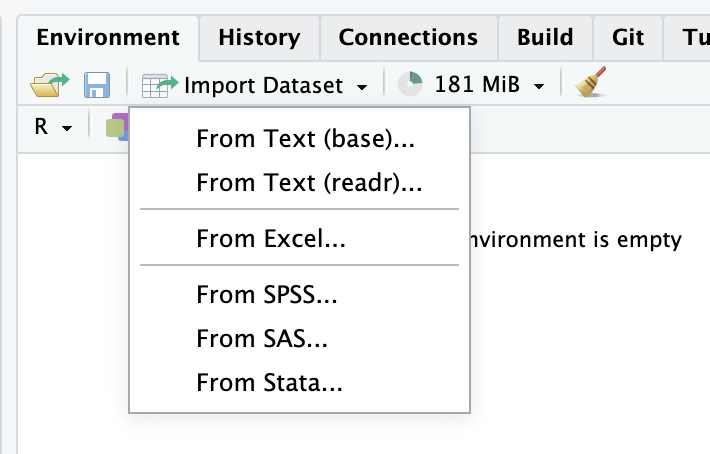
\includegraphics[width=0.4\textwidth,height=\textheight]{telaImportDataset.png}
\caption{ Figura: Importando banco de dados}
\end{figure}

\begin{itemize}
\item
  Como queremos importar um arquivo csv, a melhor opção é a segunda \textbf{From Text (readr)}
\item
  \textbf{\emph{readr}} é uma pacote do R que faz a leitura de arquivo csv (se o pacote ainda não estiver instalado no seu computador, o R fará a instalação, se você concordar!)
\end{itemize}

\begin{enumerate}
\def\labelenumi{\arabic{enumi}.}
\setcounter{enumi}{2}
\tightlist
\item
  Clicando na opção \textbf{From Text (readr)}, no botão \textbf{browser} indidique onde (no seu computador) está localizado o arquivo a ser importado. A seguinte tela será apresentada:
\end{enumerate}

\begin{figure}
\centering
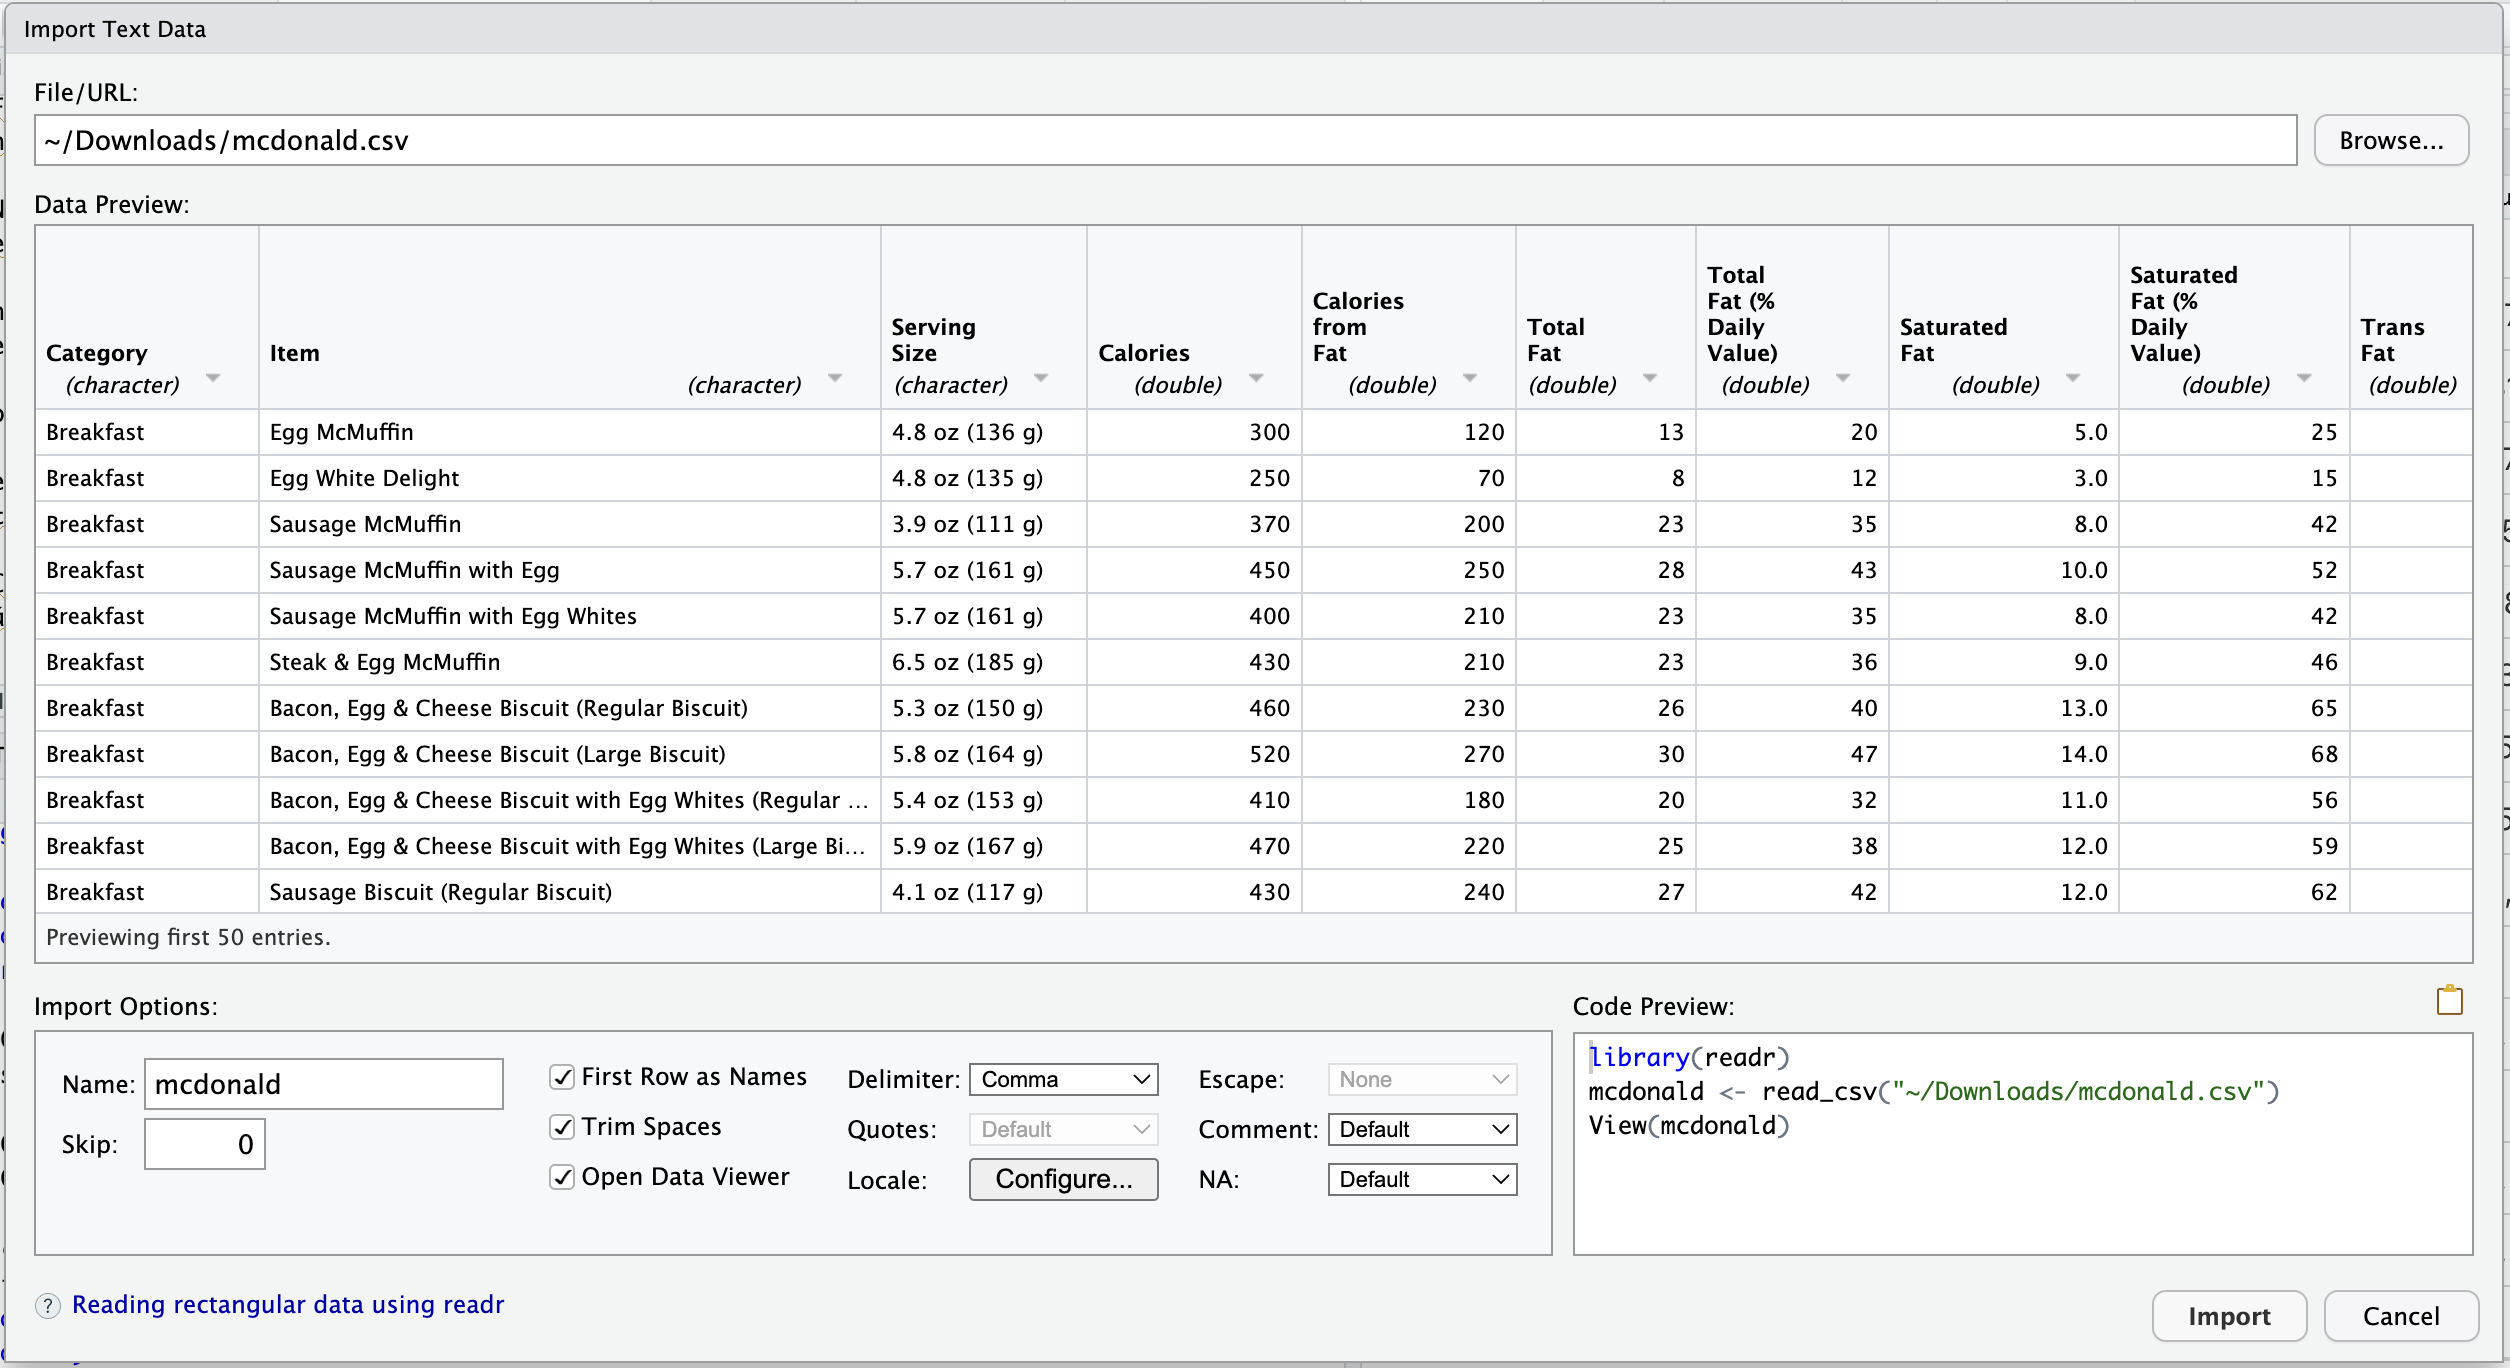
\includegraphics{telaImportBrowser.png}
\caption{ Figura: Prévia dos dados}
\end{figure}

\begin{itemize}
\item
  No quadro \textbf{Data Preview}, temos uma ``prévia'' com os nomes da variáveis, seus tipos computacionais e os primeiros valores que estão armazenados no banco de dados.
\item
  No quadro \textbf{Import Options} temos as opções de importação, fique atento ao \textbf{Name} do seu banco de dados, geralmente usamos nomes sem espaços ou caracteres especiais (', \textasciitilde{} ou ç), é até permitido usar alguns desses caracteres especiais, mas evite.
\item
  Ainda no quadro \textbf{Import Options}, observe que a opção \textbf{Open Data Viewer} está marcada, isso significa que ao importar o banco de dados, o arquivo de banco de dados será aberto pelo RStudio. Caso esteja trabalhando com bancos com muitos dados (como os bancos do dataSUS), talvez seja melhor desmarcar essa opção para não sobrecarregar o processamento do seu computador.
\item
  O quadro \textbf{Code Preview} mostra como é a importação (leitura) do banco de dados via código. É interessante copiar esse trecho de código para o arquivo de script.
\end{itemize}

\begin{enumerate}
\def\labelenumi{\arabic{enumi}.}
\setcounter{enumi}{3}
\tightlist
\item
  Clique no botão \textbf{Import} e observe que no ambiente de memória será criado o objeto do tipo \textbf{Data} com o nome do banco de dados que foi importado.
\end{enumerate}

\begin{figure}
\centering
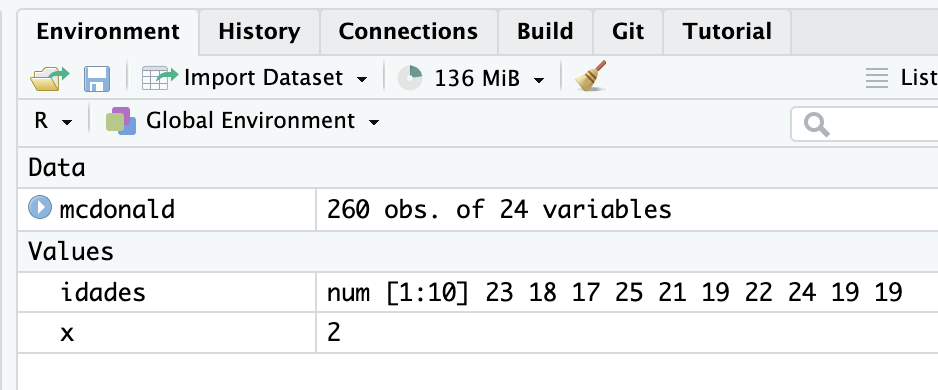
\includegraphics[width=0.6\textwidth,height=\textheight]{telaImportObjetoData.png}
\caption{ Figura: Import dataset}
\end{figure}

\begin{itemize}
\item
  Observe que esse objeto do tipo \textbf{Data} é diferente dos objetos do tipo \textbf{Values} que vimos nos exemplos iniciais.
\item
  Ao clicar no ícone ao lado do nome do objeto, temos acesso ao nomes e tipos computacionais das variáveis, e ao clicar sobre nome do objeto, o banco será aberto!
\end{itemize}

\section{Importando um banco xls}\label{importando-um-banco-xls}

Na área de ambiente de memória, localize \textbf{Import Dataset}, ao clicar sobre essa opção, escolha \textbf{From Excel\ldots{}}

\begin{figure}
\centering
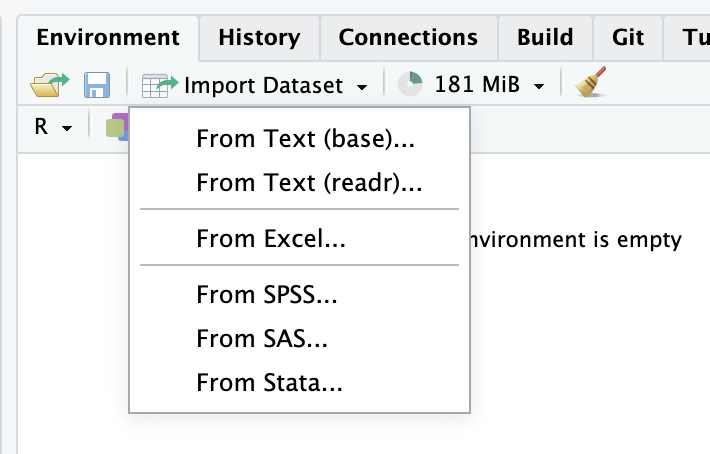
\includegraphics[width=0.4\textwidth,height=\textheight]{telaImportDataset.png}
\caption{ Figura: Importando banco de dados}
\end{figure}

\begin{itemize}
\tightlist
\item
  Se for a primeira vez que você estiver importando um arquivo Excel, pode ser necessária a instalação do pacote que fornece a biblioteca que tem a função de leitura de arquivo xls (\textbf{readxl})! O RStudio mostrará um aviso parecido com este:
\end{itemize}

\begin{figure}
\centering
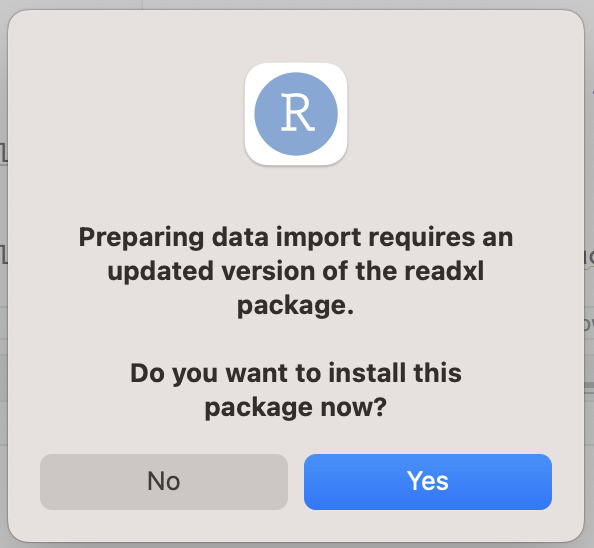
\includegraphics[width=0.4\textwidth,height=\textheight]{telaImportPacote.png}
\caption{ Figura: Aviso para instalação de pacote}
\end{figure}

\section{Exemplo 1}\label{exemplo-1-1}

Como obter a média da variável \textbf{Calories} que é uma coluna do objeto \textbf{mcdonald}, que por sua vez, é um objeto do tipo \textbf{Data}?

\begin{Shaded}
\begin{Highlighting}[]
\CommentTok{\# Usamos o operador $}
\CommentTok{\# Para calcular a média precisamos informar para função: }
\CommentTok{\# mean( NOME DO BANCO $ NOME DA COLUNA ): }
\FunctionTok{mean}\NormalTok{(mcdonald}\SpecialCharTok{$}\NormalTok{Calories)}
\end{Highlighting}
\end{Shaded}

\section{Exemplo 2}\label{exemplo-2-1}

Como armazenar os valores de uma variável (coluna), em um objeto do tipo \textbf{Values} e depois calcular a média?

\begin{Shaded}
\begin{Highlighting}[]
\CommentTok{\# Uso o operador \textless{}{-} }
\CommentTok{\# Criamos o objeto }
\NormalTok{caloria }\OtherTok{\textless{}{-}}\NormalTok{ mcdonald}\SpecialCharTok{$}\NormalTok{Calories}
\CommentTok{\# Agora podemos usar o objeto que criamos, por exemplo para calcular a média e o desvio padrão}
\FunctionTok{mean}\NormalTok{(caloria)}
\FunctionTok{sd}\NormalTok{(caloria)}
\end{Highlighting}
\end{Shaded}

\section{Exemplo 3}\label{exemplo-3-1}

O que acontece se usamos a função \textbf{summary()} para o objeto \textbf{mcdonald}, sem usar o operador, isto é sem indicar uma variável?

\begin{Shaded}
\begin{Highlighting}[]
\CommentTok{\# No console será mostrado o resumo de todas as variáveis do banco!}
\FunctionTok{summary}\NormalTok{(mcdonald)}
\end{Highlighting}
\end{Shaded}

\begin{quote}
Essa forma de obter os resultados não é a melhor forma, vamos \textbf{instalar um pacote} para obter os resultados em uma tabela bem formatada que podemos copiar e colar diretamente para um editor de texto.
\end{quote}

\chapter{Instalando pacotes}\label{instalando-pacotes}

Quando instalamos nosso ambiente computacional R e RStudio, instalamos uma versão básica, onde apenas os recursos básicos do R estão diponíveis, o pacote básico (\textbf{base}) do R.

Os pacotes (\textbf{packages}) do R são compostos por uma biblioteca (\textbf{library}) que é um conjunto de funções. Por exemplo, do pacote \textbf{base} usamos as funções min(), max(), mean(), median(), table(), var(), sd(), summary(), etc.

Para ver a lista de funções que compõem a bilbioteca do pacote base, execute o código:

\begin{Shaded}
\begin{Highlighting}[]
\FunctionTok{library}\NormalTok{(}\AttributeTok{help =} \StringTok{"base"}\NormalTok{)}
\end{Highlighting}
\end{Shaded}

Os pacotes são análogos aos aplicativos que instalamos nos nossos celulares, são módulos que agregam funcionalidades específicas. Ao longo das nossas atividades usaremos alguns desses pacotes.

Como nesse momento estamos interessados em otimizar o trabalho para realizar uma análise descritiva dos dados, então vamos instalar um pacote chamado \textbf{gtsummary} (\url{https://www.danieldsjoberg.com/gtsummary/}).

\begin{quote}
O pacote \textbf{gtsummary} nos fornecerá uma tabela resumo de todo banco de dados, otimizando bastante nosso trabalho de resumir o banco de dados.
\end{quote}

\begin{itemize}
\item
  IMPORTANTE 1: instalamos um pacote apenas uma vez (como um aplicativo no celular\ldots{} a gente só refaz a instalação se o app \emph{bugar}!)
\item
  IMPORTANTE 2: todas vez precisamos carregar o pacote com as funções que queremos usar por meio da função \textbf{library()}
\end{itemize}

Veja o código:

\begin{Shaded}
\begin{Highlighting}[]
\CommentTok{\# comando para instalar o pacote gtsummary}
\FunctionTok{install.packages}\NormalTok{(}\StringTok{"gtsummary"}\NormalTok{)}

\CommentTok{\# comando para carregar a biblioteca de funções do gtsummary}
\FunctionTok{library}\NormalTok{(gtsummary)}

\CommentTok{\# a função que vamos usar para gerar uma tabela que resume os dados é}
\CommentTok{\# tbl\_summary}
\FunctionTok{tbl\_summary}\NormalTok{(mcdonald)}
\end{Highlighting}
\end{Shaded}

\begin{itemize}
\item
  Ao executar \textbf{tbl\_summary(mcdonald)} a tabela de resultados será mostrada na área de arquivos, gráficos, pacotes\ldots{} na aba \textbf{Viewer}, no quadrante abaixo do ambiente de memória.
\item
  Essa tabela pode ser copiada e colada para o editor de texto que você utiliza para escrever seus trabalhos, claro essa tabela pode ser melhorada!
\item
  Observe no rodapé da tabela a seguinte legenda \textbf{n (\%); Median (IQR)}, isso significa que para

  \begin{itemize}
  \item
    \textbf{variáveis qualitativas:} n é a contagem (frequência absoluta) e entre parenteses (\%) é mostrado a porcentagem de cada categoria.
  \item
    \textbf{variveis quantitativas:} Median é a mediana e entre parenteses (IQR - de InterQuantile Range) estão o primeiro e terceiro quartil respectivamente.
  \end{itemize}
\end{itemize}

\section{Exemplo 1}\label{exemplo-1-2}

Como mostrar o resultado com a média e desvio padrão?

\begin{Shaded}
\begin{Highlighting}[]
\CommentTok{\# acrescente nos argumentos da função tbl\_summary() a opção:}
\CommentTok{\# statistic = list(all\_continuous() \textasciitilde{} "\{mean\} (\{sd\})"}
\FunctionTok{tbl\_summary}\NormalTok{(}
\NormalTok{            mcdonald, }
            \AttributeTok{statistic =} \FunctionTok{list}\NormalTok{(}\FunctionTok{all\_continuous}\NormalTok{() }\SpecialCharTok{\textasciitilde{}} \StringTok{"\{mean\} (\{sd\})"}\NormalTok{)}
\NormalTok{            )}
\end{Highlighting}
\end{Shaded}

\section{Exemplo 2}\label{exemplo-2-2}

Como selecionar somente algumas variáveis do banco de dados?

\begin{Shaded}
\begin{Highlighting}[]
\CommentTok{\# Precisamos do pacote tidyverse, tire o símbolo de \# se precisar instalar!}
\CommentTok{\# install.packages("tidyverse")}

\CommentTok{\# ative tidyverse}
\FunctionTok{library}\NormalTok{(tidyverse)}

\CommentTok{\# vamos usar a função select() do pacote tidyverse}
\NormalTok{dadosSelecionados }\OtherTok{\textless{}{-}} \FunctionTok{select}\NormalTok{ (mcdonald, Cholesterol, Sodium, Carbohydrates)}

\CommentTok{\# faça uma tabela para o objeto dadosSelecionados}
\FunctionTok{tbl\_summary}\NormalTok{(dadosSelecionados)}
\end{Highlighting}
\end{Shaded}

\section{Exemplo 3}\label{exemplo-3-2}

Algumas vezes é mais fácil excluir algumas variáveis, por exemplo queremos todas, menos \textbf{Item} e \textbf{Serving Size}

\begin{Shaded}
\begin{Highlighting}[]
\CommentTok{\# vamos usar a função select() do pacote tidyverse e colocar o sinal de menos ({-})}
\CommentTok{\# antes dos nomes das variáveis que queremos excluir}
\CommentTok{\# IMPORTANTE: Serving Size é um nome de variável com espaço }
\CommentTok{\# então devemos referênciá{-}la entre aspas: \textasciigrave{}Serving Size\textasciigrave{}}
\NormalTok{dadosSelecionados2 }\OtherTok{\textless{}{-}} \FunctionTok{select}\NormalTok{ (mcdonald, }\SpecialCharTok{{-}}\NormalTok{Item, }\SpecialCharTok{{-}}\StringTok{\textasciigrave{}}\AttributeTok{Serving Size}\StringTok{\textasciigrave{}}\NormalTok{)}

\CommentTok{\# faça uma tabela para o objeto dadosSelecionados2}
\FunctionTok{tbl\_summary}\NormalTok{(dadosSelecionados2)}
\end{Highlighting}
\end{Shaded}

\section{Exemplo 4}\label{exemplo-4}

Como selecinar um conjunto de variáveis que estão em sequência, por exemplo, de \textbf{Carbohydrates} a \textbf{Cholesterol (\% Daily Value)}

\begin{Shaded}
\begin{Highlighting}[]
\CommentTok{\# vamos usar a função select() do pacote tidyverse e colocar o sinal de dois pontos (:)}
\CommentTok{\# entre a primeira variável e a última da sequência }
\CommentTok{\# IMPORTANTE: Cholesterol (\% Daily Value) é um nome de variável com espaço }
\CommentTok{\# então devemos referênciá{-}la entre aspas: \textasciigrave{}Cholesterol (\% Daily Value)\textasciigrave{}}
\NormalTok{dadosSelecionados3 }\OtherTok{\textless{}{-}} \FunctionTok{select}\NormalTok{ (mcdonald, Carbohydrates}\SpecialCharTok{:}\StringTok{\textasciigrave{}}\AttributeTok{Cholesterol (\% Daily Value)}\StringTok{\textasciigrave{}}\NormalTok{)}

\CommentTok{\# faça uma tabela para o objeto dadosSelecionados}
\FunctionTok{tbl\_summary}\NormalTok{(dadosSelecionados3)}
\end{Highlighting}
\end{Shaded}

\begin{quote}
Saiba mais sobre o Tidyverse \url{https://www.tidyverse.org/packages/}
\end{quote}

\section{Atividade 5}\label{atividade-5}

\textbf{Escolha outro banco de dados (você pode até criar um banco fictício!), faça uma tabela descritiva dos dados e escreva sobre os dados (um ou dois parágrafos), afinal, o nosso trabalho não é só obter a tabela, é dissertar sobre o que essa tabela revela sobre a amostra em estudo!}

\chapter{Gráficos}\label{gruxe1ficos}

Nesse link \url{https://r-graph-gallery.com/} está algumas possibilidades de gráficos que podemos fazer usando o R. Para fazer gráficos mais elaborados (aparentemente mais atrativos visualmente) usamos o pacote \textbf{GGPlot2} \url{https://ggplot2.tidyverse.org/}.

Focaremos nossa atenção em dois gráficos específicos para variáveis quantitativas: \textbf{Histograma} e \textbf{Boxplot}, em nem faremos nada atrativo, usaremos o pacote básico do R que nos fornece as funções \textbf{hist()} e \textbf{boxplot()}, pois o nosso obtivo para esse momento é simplesmente estudar a importância desses gráficos.

O que a gente levaria um tempinho\ldots{} é simplesmente assim em código R:

\begin{Shaded}
\begin{Highlighting}[]
\NormalTok{Batimentos }\OtherTok{\textless{}{-}} \FunctionTok{c}\NormalTok{(}\DecValTok{62}\NormalTok{, }\DecValTok{55}\NormalTok{, }\DecValTok{56}\NormalTok{, }\DecValTok{46}\NormalTok{, }\DecValTok{75}\NormalTok{, }\DecValTok{67}\NormalTok{, }\DecValTok{62}\NormalTok{, }\DecValTok{75}\NormalTok{, }\DecValTok{60}\NormalTok{, }\DecValTok{54}\NormalTok{, }\DecValTok{69}\NormalTok{, }\DecValTok{63}\NormalTok{, }\DecValTok{39}\NormalTok{, }\DecValTok{57}\NormalTok{, }\DecValTok{40}\NormalTok{, }\DecValTok{39}\NormalTok{, }\DecValTok{64}\NormalTok{, }\DecValTok{71}\NormalTok{, }\DecValTok{61}\NormalTok{, }\DecValTok{54}\NormalTok{, }\DecValTok{120}\NormalTok{)}

\CommentTok{\# Para fazer o Histograma de Batimentos}
\FunctionTok{hist}\NormalTok{(Batimentos)}

\CommentTok{\# Para fazer o Boxplot de Batimentos}
\FunctionTok{boxplot}\NormalTok{(Batimentos)}
\end{Highlighting}
\end{Shaded}

Na área de gráficos (\textbf{Plots}), abaixo do ambiente de memória, serão mostrados os gráficos:

\begin{quote}
Histograma
\end{quote}

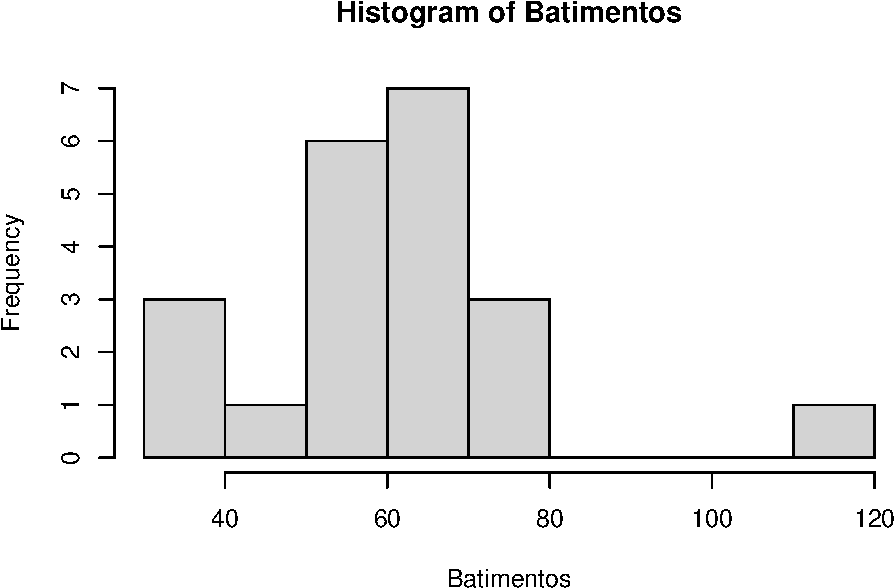
\includegraphics{Livro-Estatistica+R_files/figure-latex/unnamed-chunk-14-1.pdf}

\begin{quote}
Boxplot
\end{quote}

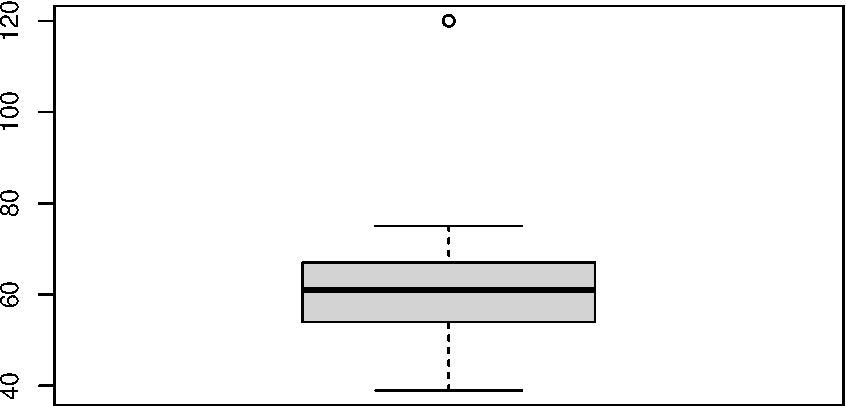
\includegraphics{Livro-Estatistica+R_files/figure-latex/unnamed-chunk-15-1.pdf}

\begin{quote}
Observações
\end{quote}

\begin{itemize}
\item
  Os gráficos mostram a informação batimentos de duas formas diferentes, mas elas estão relacionadas!
\item
  Observe que eixo horizontal do histograma corresponde ao eixo vertical do boxplot
\end{itemize}

\section{Histograma}\label{histograma}

O histograma é um gráfico que usado para variáveis quantitativas contínua.

O histograma pode nos dar uma noção do tipo de \textbf{distribuição de probabibilidade} que os dados seguem.

A ideia desse gráfico é agrupar os dados em \textbf{classes} (cada barra do histograma é uma classe) e no eixo vertical tem-se a contagem (frequência) de quantos valores foram alocados em cada classe.

Para fazer a \textbf{leitura do histograma}:

\begin{itemize}
\item
  Identifique as classes no ``eixo x''
\item
  Identifique quantos elementos tem em cada classe no ``eixo y''
\end{itemize}

Acredito que nesse exemplo, é fácil verificar:

\begin{itemize}
\item
  A segunda classe: 40 - 50 batimentos, que tem 1 elemento (verifique no objeto Batimentos)
\item
  A terceira classe: 50 - 60 batimentos, que tem 6 elementos
\item
  Então, a \textbf{aplitude das classes} é igual a 10. Logo, a primeira classe é de 30 - 40.
\item
  As classes 80 - 90; 90 - 100 e 100 - 110 não tiveram ocorrências!
\item
  A classe 110-120 possui 1 elemento, que é aquele valor discrepante em relação aos demais valores.
\end{itemize}

Se não for fácil identificar as classes (eixo x) você pode usar o comando abaixo:

\begin{Shaded}
\begin{Highlighting}[]
\CommentTok{\# Para obter as "quebras" de cada classe }
\FunctionTok{hist}\NormalTok{(Batimentos)}\SpecialCharTok{$}\NormalTok{breaks}
\end{Highlighting}
\end{Shaded}

Se não for fácil identificar as frequencias (eixo y) você pode usar o comando abaixo:

\begin{Shaded}
\begin{Highlighting}[]
\CommentTok{\# Para obter a frequência em cada classe}
\FunctionTok{hist}\NormalTok{(Batimentos)}\SpecialCharTok{$}\NormalTok{count}
\end{Highlighting}
\end{Shaded}

De fato, o que estamos lendo por meio do histograma é o que chamamos de \textbf{tabela de frequência}:

\begin{longtable}[]{@{}cc@{}}
\toprule\noalign{}
Classe & Frequência \\
\midrule\noalign{}
\endhead
\bottomrule\noalign{}
\endlastfoot
30 - 40 & 3 \\
40 - 50 & 1 \\
50 - 60 & 6 \\
60 - 70 & 7 \\
70 - 80 & 3 \\
80 - 90 & 0 \\
90 - 100 & 0 \\
100 - 110 & 0 \\
110 - 120 & 1 \\
\(\sum n\) & 21 \\
\end{longtable}

\begin{itemize}
\item
  Por meio do histograma ou da tabela podemos concluir que a classe modal (moda) é a classe de 60 - 70 batimentos;
\item
  A frequência foi apresentada em termos absolutos mais pode ser transformada em frequência percentual.
\item
  Quando estamos aprendendo a fazer um histograma manualmente, primeiro construímos essa tabela de frenquência, e para construí-la é necessário calcular o número ótimo de classes, umas das regras mais usada é a Regra Sturges (essa é opção padrão do R).
\end{itemize}

Podemos usar o pacote básico R para melhorar a aparência desse gráfico.

\begin{Shaded}
\begin{Highlighting}[]
\NormalTok{hisBat }\OtherTok{\textless{}{-}} \FunctionTok{hist}\NormalTok{(Batimentos,}
               \AttributeTok{main =} \StringTok{"Histograma"}\NormalTok{,}
               \AttributeTok{xlab =} \StringTok{"Batimentos cardíacos"}\NormalTok{,}
               \AttributeTok{sub =} \StringTok{"por classes"}\NormalTok{,}
               \AttributeTok{ylab =} \StringTok{"Frequência absoluta"}\NormalTok{,}
               \AttributeTok{xlim =} \FunctionTok{c}\NormalTok{(}\DecValTok{20}\NormalTok{, }\DecValTok{120}\NormalTok{),}
               \AttributeTok{ylim =} \FunctionTok{c}\NormalTok{(}\DecValTok{0}\NormalTok{, }\DecValTok{8}\NormalTok{),}
               \AttributeTok{col =} \StringTok{"lightgreen"}\NormalTok{)}
\FunctionTok{text}\NormalTok{(hisBat}\SpecialCharTok{$}\NormalTok{mids, hisBat}\SpecialCharTok{$}\NormalTok{counts, }\AttributeTok{labels=}\NormalTok{hisBat}\SpecialCharTok{$}\NormalTok{counts, }\AttributeTok{adj =} \FunctionTok{c}\NormalTok{(}\FloatTok{0.5}\NormalTok{,}\SpecialCharTok{{-}}\FloatTok{0.5}\NormalTok{))}

\CommentTok{\# adicionar linha para indicar a média}
\FunctionTok{abline}\NormalTok{(}\AttributeTok{v =} \FunctionTok{mean}\NormalTok{(Batimentos),                      }
       \AttributeTok{col =} \StringTok{"red"}\NormalTok{,}
       \AttributeTok{lwd =} \DecValTok{3}\NormalTok{)}
\end{Highlighting}
\end{Shaded}

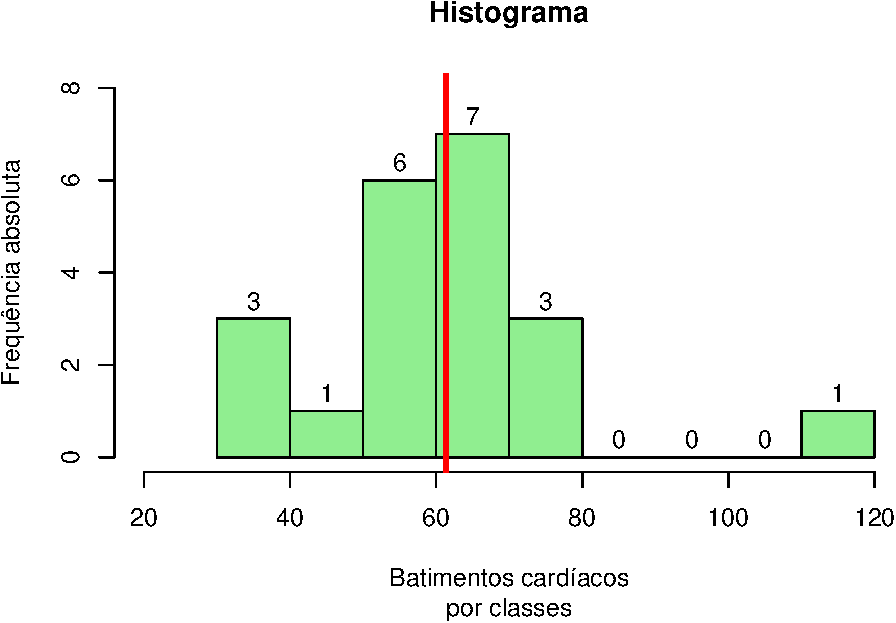
\includegraphics{Livro-Estatistica+R_files/figure-latex/unnamed-chunk-18-1.pdf}

\section{Boxplot}\label{boxplot}

Boxplot ou diagrama de caixa, é um gráfico que mostra as medidas: menor valor, primeiro quartil, mediana, terceiro quartil e máximo valor.

\begin{itemize}
\tightlist
\item
  Valores discrepantes (\emph{outliers}) são detectados pelo boxplot. Veja a figura:
\end{itemize}

\begin{figure}
\centering
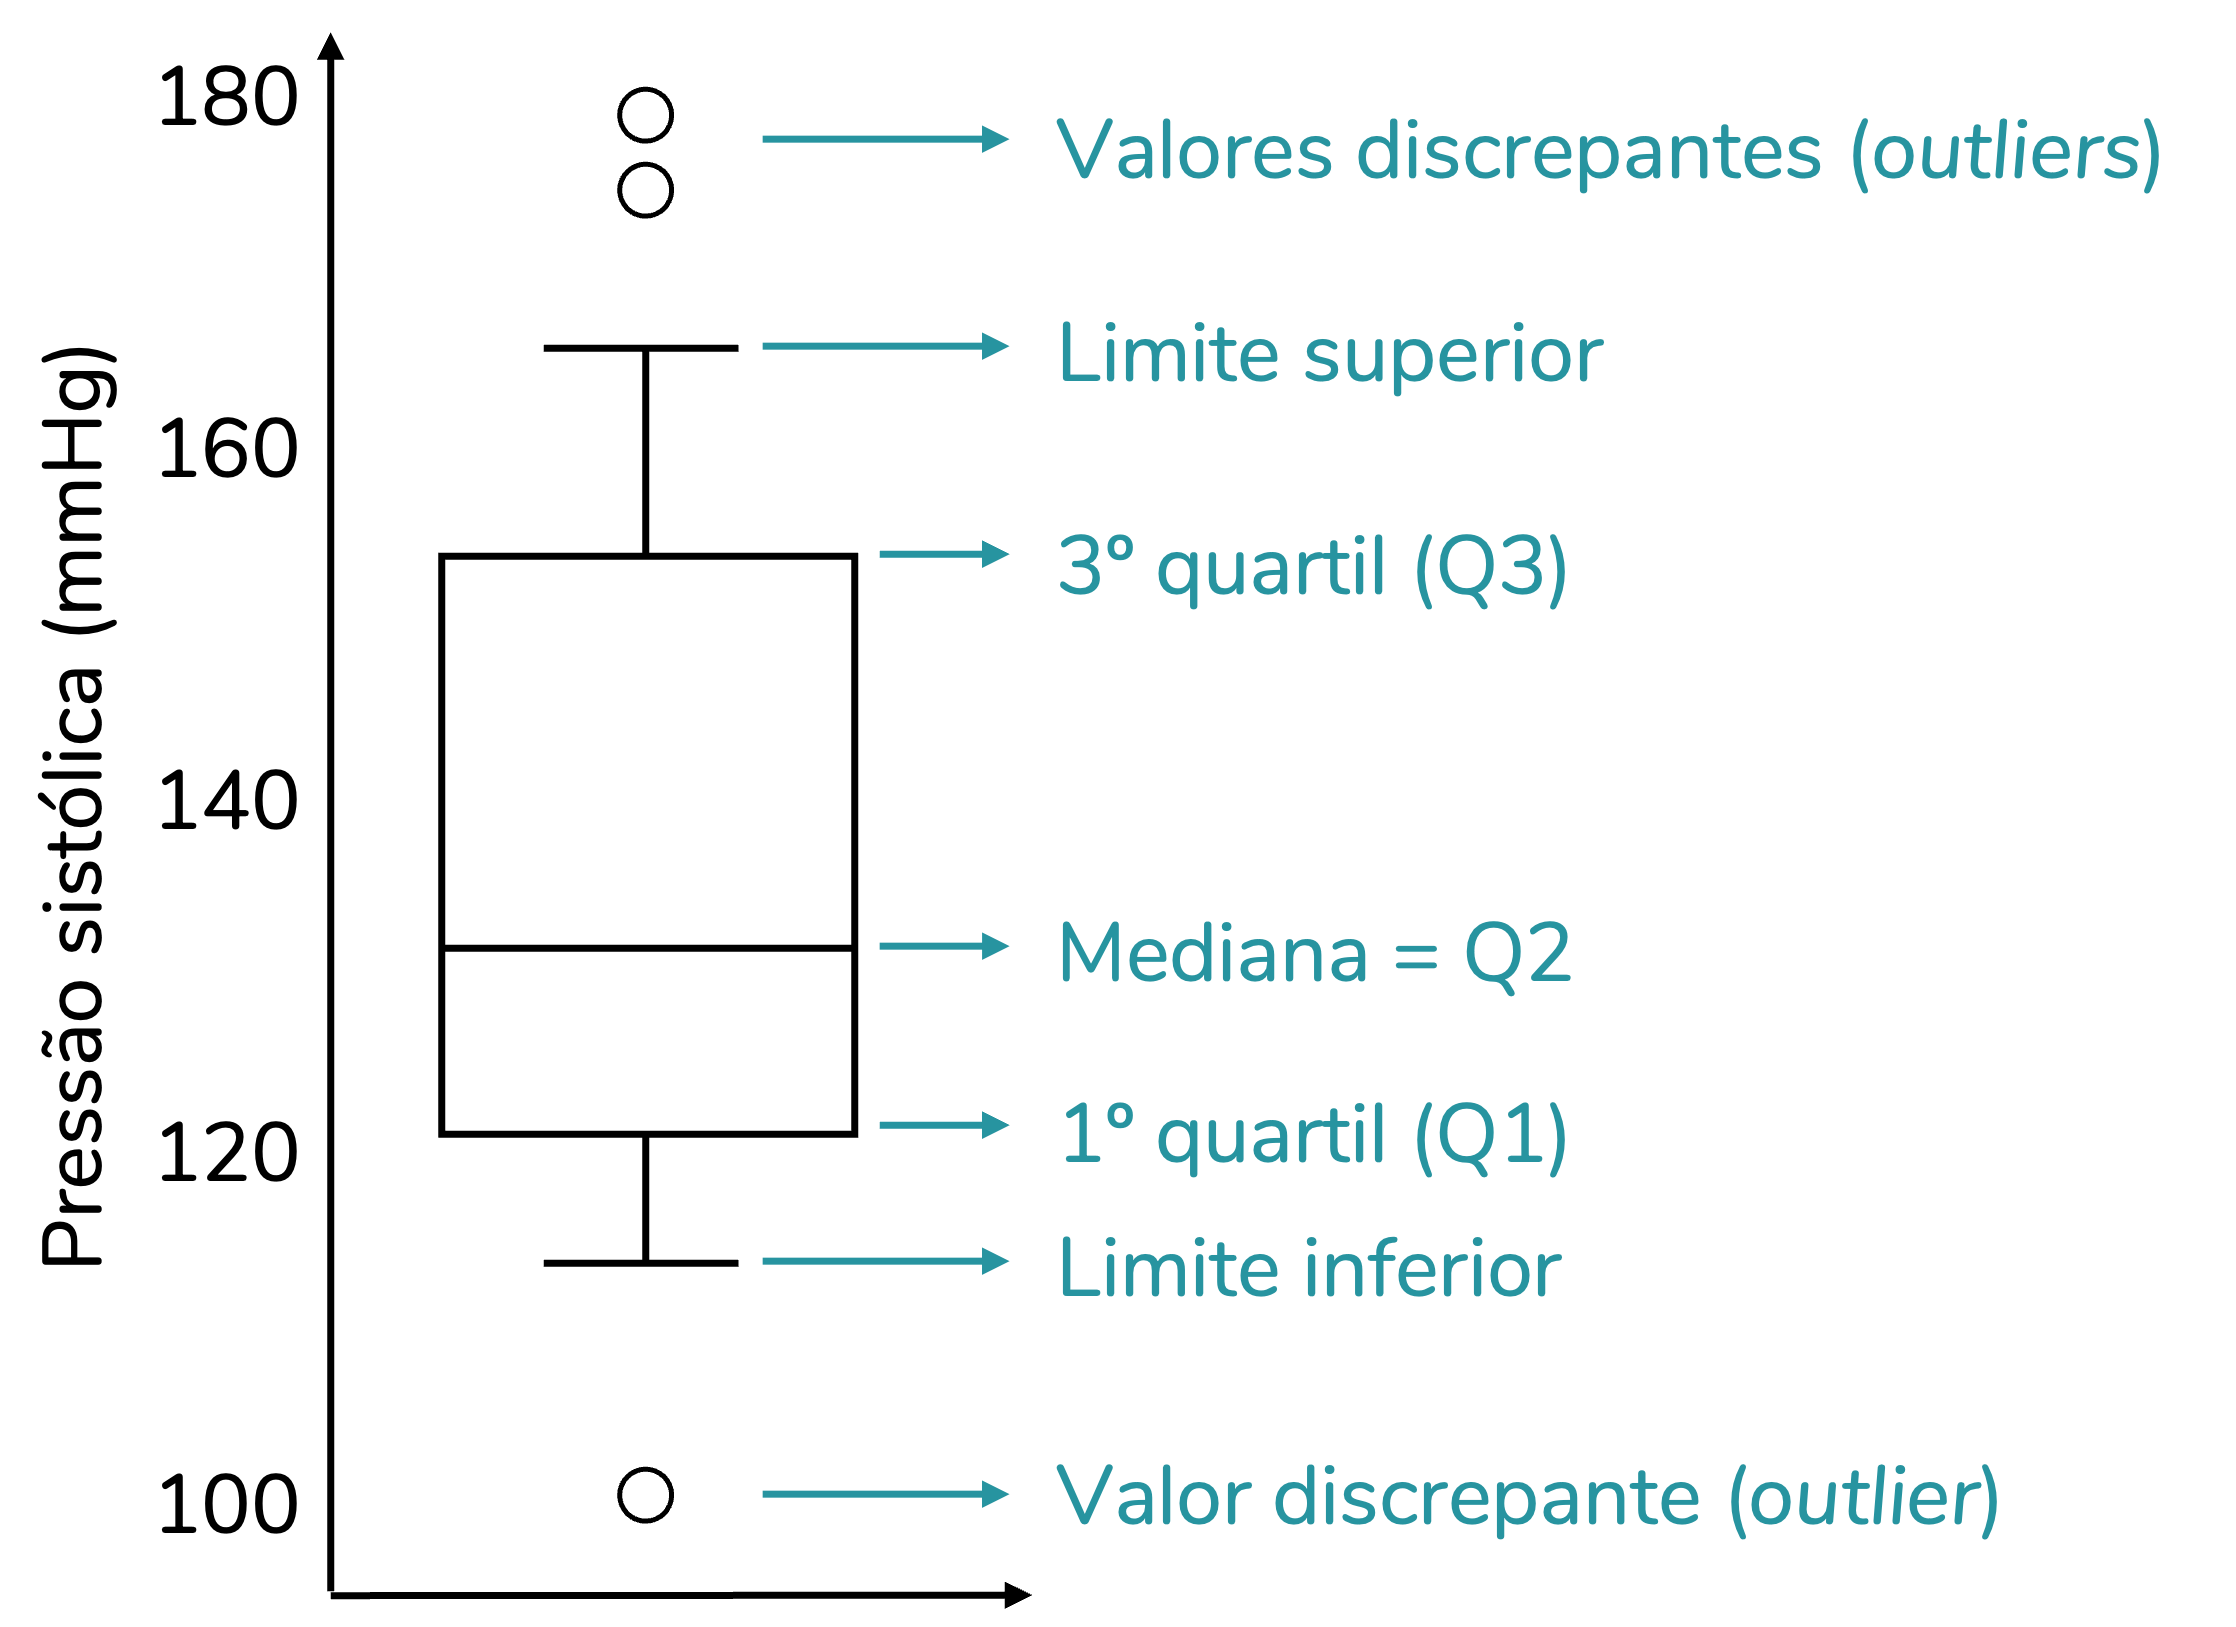
\includegraphics[width=0.5\textwidth,height=\textheight]{Boxplotexemplo.png}
\caption{Figura: ``Anatomia de um boxplot''}
\end{figure}

Essa figura foi retirada do site da Prof.~Fernanda \url{https://fernandafperes.com.br/blog/interpretacao-boxplot/} (uma exelente referência para estudar estatística!)

\begin{quote}
Geralmente eles são representados na vertical, mas também é comum a representação na horizontal.
\end{quote}

\begin{Shaded}
\begin{Highlighting}[]
\CommentTok{\# Para fazer o Boxplot de Batimentos na horizontal}
\FunctionTok{boxplot}\NormalTok{(Batimentos, }\AttributeTok{horizontal =} \ConstantTok{TRUE}\NormalTok{)}
\end{Highlighting}
\end{Shaded}

\begin{quote}
É uma forma de comparar dois grupos em relação a uma medida, por exemplo os batimentos cardiacos de grupo de homens e de mulheres
\end{quote}

\begin{Shaded}
\begin{Highlighting}[]
\CommentTok{\# Geração de amostras simuladas}
\FunctionTok{set.seed}\NormalTok{(}\DecValTok{1}\NormalTok{)}
\NormalTok{BatimentosMulheres }\OtherTok{\textless{}{-}} \FunctionTok{rnorm}\NormalTok{(}\DecValTok{30}\NormalTok{, }\DecValTok{70}\NormalTok{, }\DecValTok{3}\NormalTok{)}
\NormalTok{BatimentosHomens }\OtherTok{\textless{}{-}} \FunctionTok{rnorm}\NormalTok{(}\DecValTok{30}\NormalTok{, }\DecValTok{75}\NormalTok{, }\DecValTok{8}\NormalTok{)}
\CommentTok{\# Boxplot para os dois grupos Homens e Mulheres }
\FunctionTok{boxplot}\NormalTok{(BatimentosHomens, BatimentosMulheres)}
\end{Highlighting}
\end{Shaded}

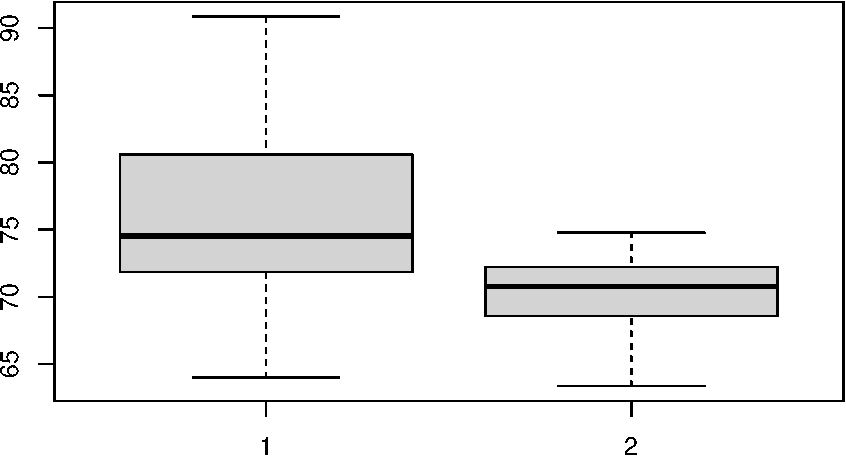
\includegraphics{Livro-Estatistica+R_files/figure-latex/unnamed-chunk-20-1.pdf}

\begin{quote}
O boxplot também pode nos informar se uma distribuição de probabilidade é simétrica ou não. Analise os gráficos abaixo, veja a conexão entre histograma e boxplot.
\end{quote}

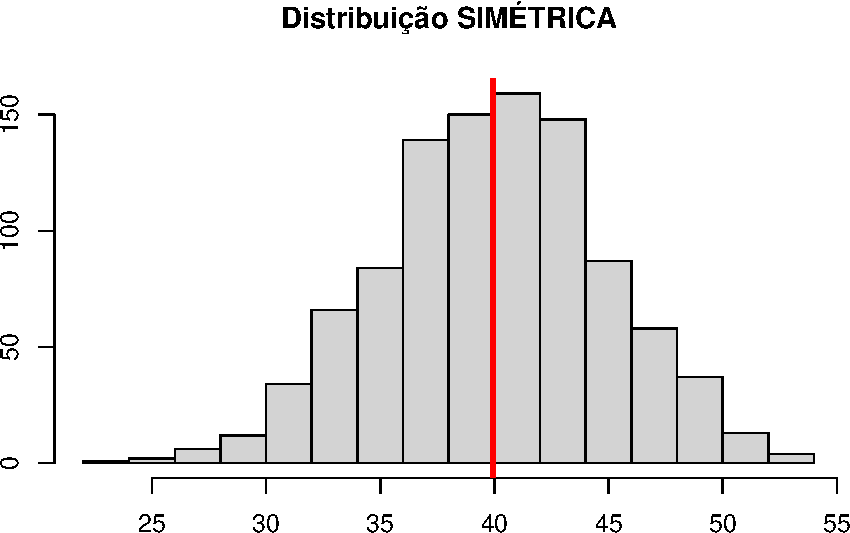
\includegraphics{Livro-Estatistica+R_files/figure-latex/unnamed-chunk-21-1.pdf}

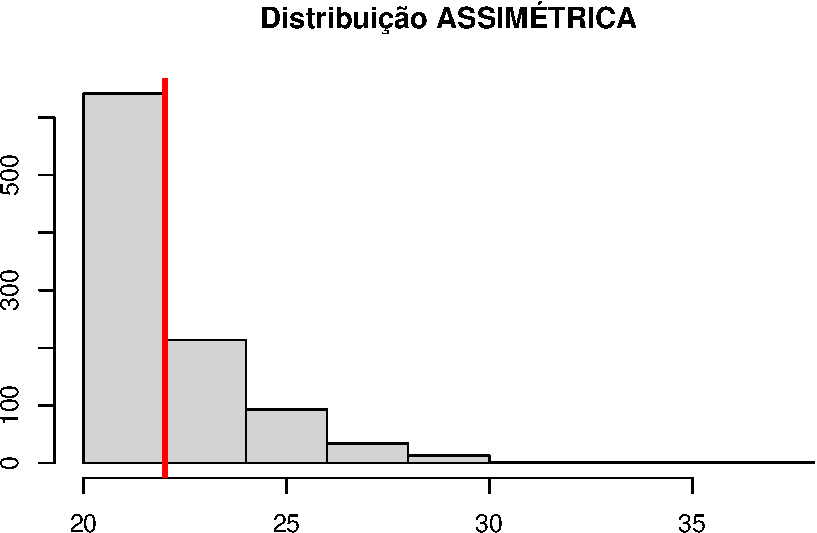
\includegraphics{Livro-Estatistica+R_files/figure-latex/unnamed-chunk-22-1.pdf} 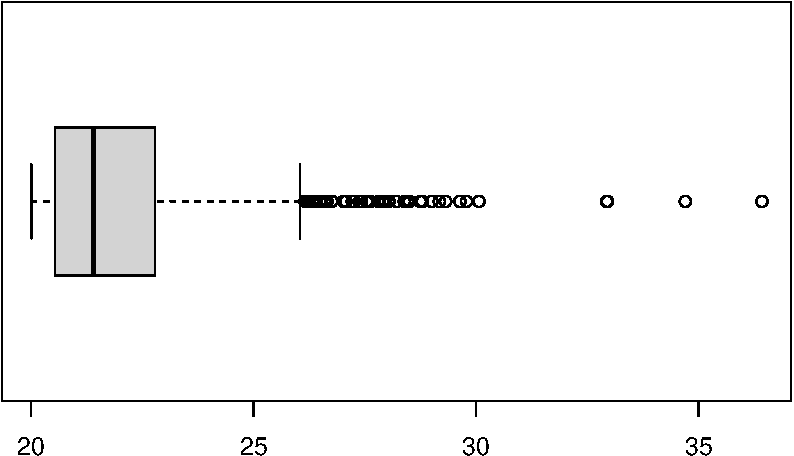
\includegraphics{Livro-Estatistica+R_files/figure-latex/unnamed-chunk-22-2.pdf}

\begin{verbatim}
##    Min. 1st Qu.  Median    Mean 3rd Qu.    Max. 
##   20.00   20.54   21.40   22.01   22.78   36.42
\end{verbatim}

\section{Atividade 6}\label{atividade-6}

\textbf{Para o banco de dados escolhido na atividade 5, faça gráficos como o histograma e boxplot, além disso, pesquise outras formas de fazer gráficos no R.}

\chapter{Distribuição de Probabilidade}\label{distribuiuxe7uxe3o-de-probabilidade}

Uma distribuição de probabilidade é um modelo matemático que descreve a relação entre os valores possíveis de uma variável e as probabilidades de ocorrência desses valores. Essencialmente, ela nos permite prever a probabilidade de eventos com base em um conjunto de dados.

Entre as distribuições mais comuns, destacam-se:

\begin{itemize}
\tightlist
\item
  Distribuição Normal (ou Gaussiana)
\item
  Distribuição Binomial
\item
  Distribuição Poisson
\item
  Distribuição Exponencial
\item
  Distribuição Uniforme
\item
  Distribuição Qui-quadrado
\item
  Distribuição t-Student
\item
  Distribuição Gama, entre outras.
\end{itemize}

Cada tipo de distribuição possui características próprias e é aplicada em diferentes contextos. A distribuição normal é uma das mais amplamente utilizadas, especialmente para modelar fenômenos naturais e sociais, como a altura de indivíduos ou o tempo de vida de produtos.

\begin{quote}
\textbf{Propriedades Gerais das Distribuições de Probabilidade}
\end{quote}

\begin{itemize}
\tightlist
\item
  \textbf{Área total sob a curva é igual a 1:} Isso significa que a soma de todas as probabilidades possíveis de ocorrência dos eventos é igual a 100\%.
\item
  \textbf{A área sob a curva representa a probabilidade de um evento.} Por exemplo, a probabilidade de um evento ocorrer entre dois valores quaisquer pode ser calculada pela área sob a curva entre esses dois pontos.
\end{itemize}

\section{Distribuição Normal}\label{distribuiuxe7uxe3o-normal}

A distribuição normal é uma das mais conhecidas na estatística. Ela modela fenômenos que seguem um comportamento simétrico em torno de uma média. A distribuição normal tem várias aplicações, desde a análise de medidas biológicas (como a pressão arterial) até a previsão de fenômenos econômicos (como o preço das ações).

\begin{quote}
\textbf{A distribuição normal é definida por dois parâmetros principais:}
\end{quote}

\begin{itemize}
\tightlist
\item
  \textbf{Média (μ):} Representa o valor central da distribuição.
\item
  \textbf{Desvio Padrão (σ):} Mede a dispersão dos dados em relação à média.
\end{itemize}

\begin{quote}
\textbf{Características da Distribuição Normal}
\end{quote}

\begin{itemize}
\tightlist
\item
  \textbf{Forma de sino:} A distribuição normal tem a forma de um sino simétrico, com a maior concentração de dados perto da média.
\item
  \textbf{Simetria:} A distribuição é simétrica em relação à média.
\item
  \textbf{Média, Mediana e Moda:} Para uma distribuição normal, a média, mediana e moda são ``iguais'' e localizam-se no centro da distribuição.
\end{itemize}

\begin{quote}
\textbf{Teoricamente o comportamento da Distribuição Normal é dado por:}
\end{quote}

\begin{figure}
\centering
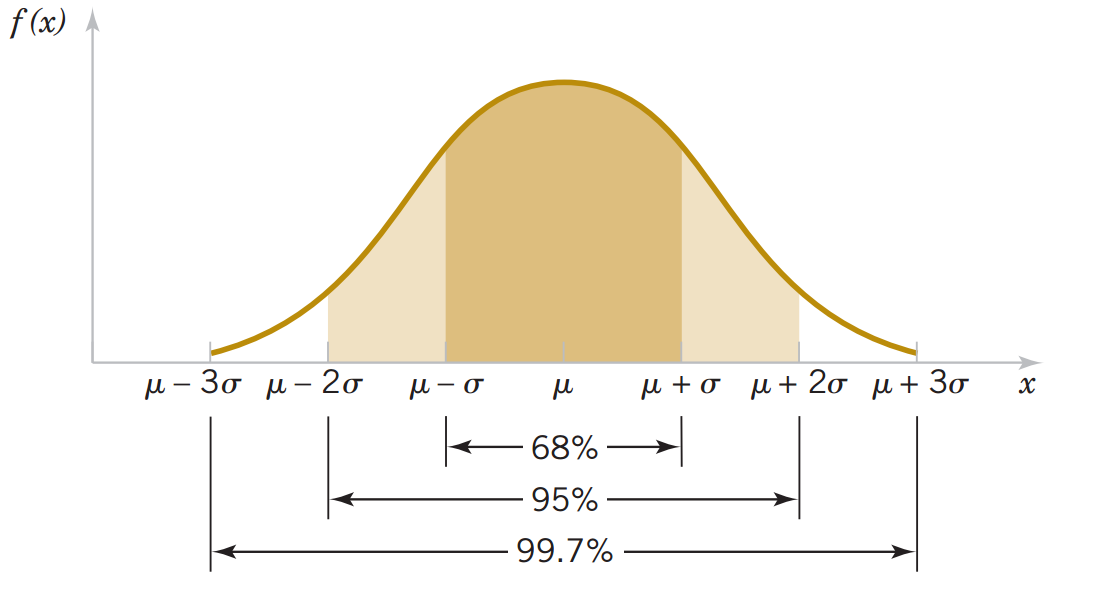
\includegraphics[width=0.8\textwidth,height=\textheight]{normalTeorica.png}
\caption{Figura: Distribuição Normal teórica (Fonte: \url{https://www.inf.ufsc.br/~andre.zibetti/probabilidade/figures/normal.PNG})}
\end{figure}

Onde:

\begin{itemize}
\tightlist
\item
  A média está representada por \(\mu\)
\item
  O devio padrão está representado por \(\sigma\)
\end{itemize}

\begin{quote}
\textbf{Regra empirica 68\% - 95\% - 99,7\%}
Se os dados seguem uma distribuição normal, é possível fazer afirmações sobre a concentração dos dados em torno da média, conforme a regra empírica:
\end{quote}

\begin{itemize}
\tightlist
\item
  \emph{68\%} dos dados estão no intervalo de uma vez o desvio padrão (μ ± 1σ).
\item
  \emph{95\%} dos dados estão no intervalo de duas vezes o desvio padrão (μ ± 2σ).
\item
  \emph{99,7\%} dos dados estão no intervalo de três vezes o desvio padrão (μ ± 3σ).
\end{itemize}

\textbf{Importante:} Dados fora do intervalo de μ ± 3σ são considerados raros.

\begin{quote}
Exemplo de distribuição Normal, com dados simulados usado a função rnorm().
\end{quote}

\begin{Shaded}
\begin{Highlighting}[]
\CommentTok{\# semente de geração de números aleatórios }
\FunctionTok{set.seed}\NormalTok{(}\DecValTok{1}\NormalTok{)}

\CommentTok{\# Será simulada uma amostra com a seguinte característica:}
\CommentTok{\# 1000 valores}
\CommentTok{\# média \textasciitilde{} 70}
\CommentTok{\# desvio padrão \textasciitilde{} 3}
\CommentTok{\# A função rnorm() gera números randômicos com comportamento de uma distribuição Normal }
\NormalTok{BatimentosMulheres }\OtherTok{\textless{}{-}} \FunctionTok{rnorm}\NormalTok{(}\DecValTok{1000}\NormalTok{, }\DecValTok{70}\NormalTok{, }\DecValTok{3}\NormalTok{)}

\CommentTok{\# Arrendodamento com nenhuma casa depois da vírugula}
\NormalTok{BatimentosMulheres }\OtherTok{\textless{}{-}} \FunctionTok{round}\NormalTok{(BatimentosMulheres,}\DecValTok{0}\NormalTok{)}

\CommentTok{\# histograma}
\FunctionTok{hist}\NormalTok{(BatimentosMulheres)}
\end{Highlighting}
\end{Shaded}

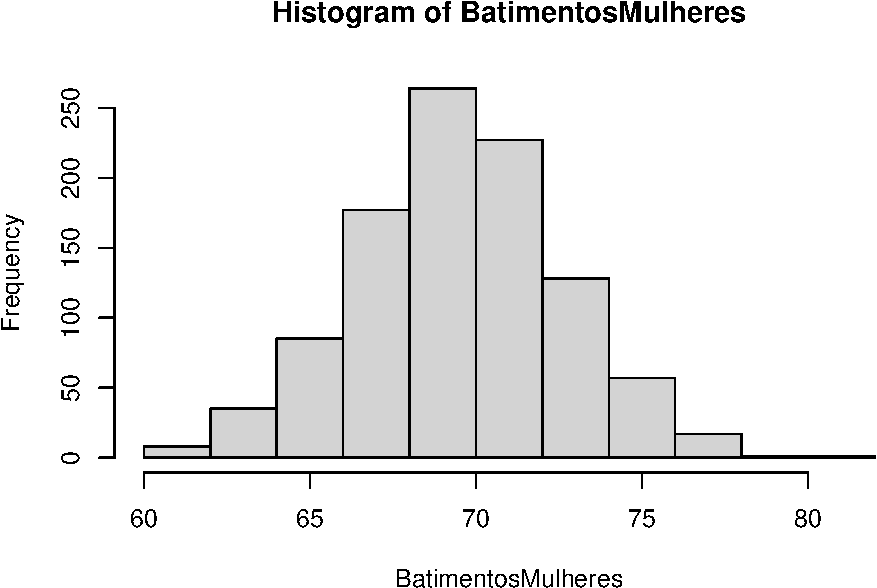
\includegraphics{Livro-Estatistica+R_files/figure-latex/unnamed-chunk-23-1.pdf}

\begin{Shaded}
\begin{Highlighting}[]
\CommentTok{\# Classes e frequencias do histograma}
\FunctionTok{hist}\NormalTok{(BatimentosMulheres)}\SpecialCharTok{$}\NormalTok{breaks}
\end{Highlighting}
\end{Shaded}

\begin{verbatim}
##  [1] 60 62 64 66 68 70 72 74 76 78 80 82
\end{verbatim}

\begin{Shaded}
\begin{Highlighting}[]
\FunctionTok{hist}\NormalTok{(BatimentosMulheres)}\SpecialCharTok{$}\NormalTok{count}
\end{Highlighting}
\end{Shaded}

\begin{verbatim}
##  [1]   8  35  85 177 264 227 128  57  17   1   1
\end{verbatim}

\begin{Shaded}
\begin{Highlighting}[]
\CommentTok{\# histograma e curva de densidade (da Dist. Normal)}
\FunctionTok{hist}\NormalTok{(BatimentosMulheres, }\AttributeTok{prob =} \ConstantTok{TRUE}\NormalTok{)}
\FunctionTok{lines}\NormalTok{(}\FunctionTok{density}\NormalTok{(BatimentosMulheres), }\AttributeTok{col =} \DecValTok{4}\NormalTok{, }\AttributeTok{lwd =} \DecValTok{2}\NormalTok{)}

\CommentTok{\# idicação da média}
\FunctionTok{abline}\NormalTok{(}\AttributeTok{v =} \FunctionTok{mean}\NormalTok{(BatimentosMulheres), }\AttributeTok{col =} \DecValTok{2}\NormalTok{, }\AttributeTok{lwd =} \DecValTok{3}\NormalTok{)}
\end{Highlighting}
\end{Shaded}

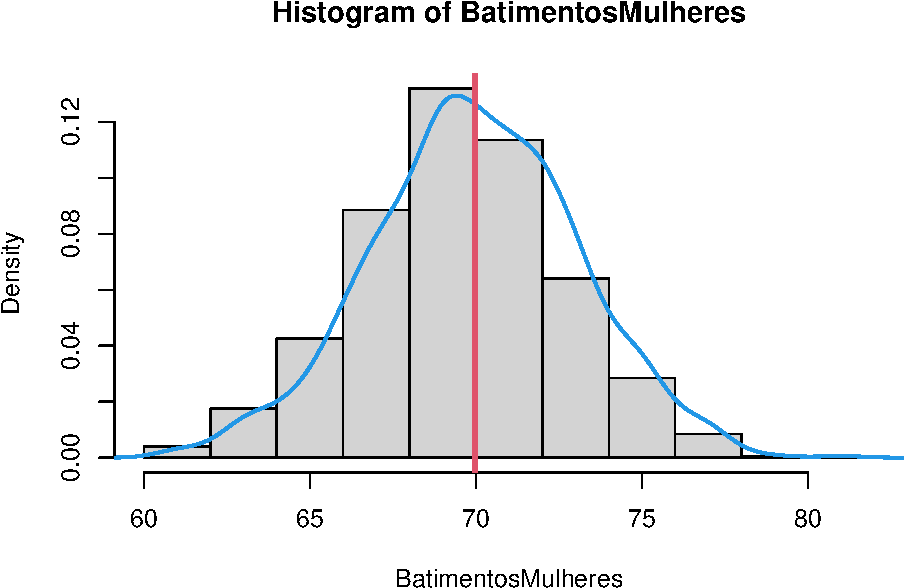
\includegraphics{Livro-Estatistica+R_files/figure-latex/unnamed-chunk-23-2.pdf}

\begin{Shaded}
\begin{Highlighting}[]
\CommentTok{\# medidas resumo}
\FunctionTok{summary}\NormalTok{(BatimentosMulheres)}
\end{Highlighting}
\end{Shaded}

\begin{verbatim}
##    Min. 1st Qu.  Median    Mean 3rd Qu.    Max. 
##   61.00   68.00   70.00   69.97   72.00   81.00
\end{verbatim}

\begin{Shaded}
\begin{Highlighting}[]
\FunctionTok{sort}\NormalTok{(}\FunctionTok{table}\NormalTok{(BatimentosMulheres), }\AttributeTok{decreasing =}\NormalTok{ T)}
\end{Highlighting}
\end{Shaded}

\begin{verbatim}
## BatimentosMulheres
##  69  70  71  72  68  67  73  66  74  75  65  64  63  76  77  61  62  78  79  81 
## 138 126 116 111  95  82  82  56  46  41  29  18  17  16  15   4   4   2   1   1
\end{verbatim}

\begin{Shaded}
\begin{Highlighting}[]
\FunctionTok{sd}\NormalTok{(BatimentosMulheres)}
\end{Highlighting}
\end{Shaded}

\begin{verbatim}
## [1] 3.10594
\end{verbatim}

\begin{Shaded}
\begin{Highlighting}[]
\CommentTok{\# CV em \%}
\FunctionTok{sd}\NormalTok{(BatimentosMulheres)}\SpecialCharTok{/}\FunctionTok{mean}\NormalTok{(BatimentosMulheres)}\SpecialCharTok{*}\DecValTok{100}
\end{Highlighting}
\end{Shaded}

\begin{verbatim}
## [1] 4.438833
\end{verbatim}

\begin{quote}
As funções \textbf{pnorm()} e \textbf{dnorm()} são usadas para calcular a probabilidade de um evento que segue uma distribuição, a qual conhecemos a média e o desvio padrão.
\end{quote}

\textbf{Exemplo:} Sabendo que os batimentos cardíacos de mulheres de 18 a 65 anos tem média de 70bmp e desvio padrão igual a 3bmp.

Calcule as probabilidades:

\begin{itemize}
\tightlist
\item
  de uma mulher ter batimentos inferior a 70bmp, ou seja, \(P(x<70)\):
\end{itemize}

\begin{Shaded}
\begin{Highlighting}[]
\CommentTok{\# pnorm(): Calcula a probabilidade acumulada até um valor específico. Ou seja, retorna a probabilidade de que uma variável aleatória, que segue uma distribuição normal, seja menor ou igual a um determinado valor.}

\CommentTok{\# observação: a resposta é 0.5 pois a média 70.}
\FunctionTok{pnorm}\NormalTok{(}\DecValTok{70}\NormalTok{, }\DecValTok{70}\NormalTok{, }\DecValTok{3}\NormalTok{)}
\end{Highlighting}
\end{Shaded}

\begin{verbatim}
## [1] 0.5
\end{verbatim}

\begin{itemize}
\tightlist
\item
  de uma mulher ter batimentos superior a 70bmp, ou seja, \(P(x>70)\):
\end{itemize}

\begin{Shaded}
\begin{Highlighting}[]
\CommentTok{\# observação: 1 é o valor da área total}
\CommentTok{\# a pnorm() fornece a área á esquerda}
\DecValTok{1} \SpecialCharTok{{-}} \FunctionTok{pnorm}\NormalTok{(}\DecValTok{70}\NormalTok{, }\DecValTok{70}\NormalTok{, }\DecValTok{3}\NormalTok{)}
\end{Highlighting}
\end{Shaded}

\begin{verbatim}
## [1] 0.5
\end{verbatim}

\begin{itemize}
\tightlist
\item
  de uma mulher ter batimentos igual a 70bmp, ou seja, \(P(x=70)\):
\end{itemize}

\begin{Shaded}
\begin{Highlighting}[]
\CommentTok{\# dnorm(): Calcula a densidade de probabilidade de um valor específico em uma distribuição normal. Em outras palavras, ela retorna o valor da função densidade de probabilidade no ponto especificado.}
\FunctionTok{dnorm}\NormalTok{(}\DecValTok{70}\NormalTok{, }\DecValTok{70}\NormalTok{, }\DecValTok{3}\NormalTok{)}
\end{Highlighting}
\end{Shaded}

\begin{verbatim}
## [1] 0.1329808
\end{verbatim}

\begin{itemize}
\tightlist
\item
  de uma mulher ter batimentos entre 67 e 73bmp \(P(67 < x < 73)\):
\end{itemize}

\begin{Shaded}
\begin{Highlighting}[]
\CommentTok{\# Observe que estamos testando a regra empírica (68\%)}
\FunctionTok{pnorm}\NormalTok{(}\DecValTok{73}\NormalTok{, }\DecValTok{70}\NormalTok{, }\DecValTok{3}\NormalTok{) }\SpecialCharTok{{-}} \FunctionTok{pnorm}\NormalTok{(}\DecValTok{67}\NormalTok{, }\DecValTok{70}\NormalTok{, }\DecValTok{3}\NormalTok{)}
\end{Highlighting}
\end{Shaded}

\begin{verbatim}
## [1] 0.6826895
\end{verbatim}

\begin{itemize}
\tightlist
\item
  de uma mulher ter batimentos entre 67 e 73bmp \(P(64 < x < 76)\):
\end{itemize}

\begin{Shaded}
\begin{Highlighting}[]
\CommentTok{\# Observe que estamos testando a regra empírica (95\%)}
\FunctionTok{pnorm}\NormalTok{(}\DecValTok{76}\NormalTok{, }\DecValTok{70}\NormalTok{, }\DecValTok{3}\NormalTok{) }\SpecialCharTok{{-}} \FunctionTok{pnorm}\NormalTok{(}\DecValTok{64}\NormalTok{, }\DecValTok{70}\NormalTok{, }\DecValTok{3}\NormalTok{)}
\end{Highlighting}
\end{Shaded}

\begin{verbatim}
## [1] 0.9544997
\end{verbatim}

\begin{itemize}
\tightlist
\item
  de uma mulher ter batimentos entre 61 e 79bmp \(P(61 < x < 79)\):
\end{itemize}

\begin{Shaded}
\begin{Highlighting}[]
\CommentTok{\# Observe que estamos testando a regra empírica (99,7\%)}
\FunctionTok{pnorm}\NormalTok{(}\DecValTok{79}\NormalTok{, }\DecValTok{70}\NormalTok{, }\DecValTok{3}\NormalTok{) }\SpecialCharTok{{-}} \FunctionTok{pnorm}\NormalTok{(}\DecValTok{61}\NormalTok{, }\DecValTok{70}\NormalTok{, }\DecValTok{3}\NormalTok{)}
\end{Highlighting}
\end{Shaded}

\begin{verbatim}
## [1] 0.9973002
\end{verbatim}

\begin{itemize}
\tightlist
\item
  de uma mulher ter batimentos maior que 90bmp \(P(x > 90)\):
\end{itemize}

\begin{Shaded}
\begin{Highlighting}[]
\CommentTok{\# Um evento raro}
\DecValTok{1} \SpecialCharTok{{-}} \FunctionTok{pnorm}\NormalTok{(}\DecValTok{90}\NormalTok{, }\DecValTok{70}\NormalTok{, }\DecValTok{3}\NormalTok{)}
\end{Highlighting}
\end{Shaded}

\begin{verbatim}
## [1] 1.308398e-11
\end{verbatim}

\begin{itemize}
\tightlist
\item
  de uma mulher ter batimentos menor que 65bmp \(P(x < 65)\):
\end{itemize}

\begin{Shaded}
\begin{Highlighting}[]
\FunctionTok{pnorm}\NormalTok{(}\DecValTok{65}\NormalTok{, }\DecValTok{70}\NormalTok{, }\DecValTok{3}\NormalTok{)}
\end{Highlighting}
\end{Shaded}

\begin{verbatim}
## [1] 0.04779035
\end{verbatim}

\section{Gráfico QQ}\label{gruxe1fico-qq}

Uma maneira comum de verificar a normalidade de uma distribuição é utilizando o gráfico QQ. Ele compara os quantis de uma amostra com os quantis de uma distribuição normal padrão, e é muito útil para identificar se os dados seguem uma distribuição normal.

\begin{quote}
\textbf{Distribuição Normal Padrão}
\end{quote}

A distribuição normal padrão tem duas características importantes:

\begin{itemize}
\tightlist
\item
  Média (μ) igual a 0
\item
  Desvio padrão (σ) igual a 1
\end{itemize}

\begin{quote}
\textbf{Cálculo do Escore Z}
\end{quote}

Qualquer distribuição normal pode ser transformada na distribuição normal padrão utilizando o escore Z. O \textbf{escore Z} é calculado pela fórmula:

\[
z = \frac{(x - \mu)}{\sigma}
\]

Onde:

\begin{itemize}
\tightlist
\item
  \(x\) é o valor da observação.
\item
  \(\mu\) é a média da distribuição.
\item
  \(\sigma\) é o desvio padrão da distribuição.
\end{itemize}

O gráfico QQ realiza exatamente o que a fórmula do escore Z descreve: ele transforma os dados da amostra para a distribuição normal padrão (média 0 e desvio padrão 1) e então compara esses valores transformados com os quantis da distribuição normal teórica. Se os pontos formarem uma linha reta, isso sugere que os dados seguem uma distribuição normal.

Veja um exemplo no R para uma Distribuição Normal Padrão:

\begin{Shaded}
\begin{Highlighting}[]
\FunctionTok{set.seed}\NormalTok{(}\DecValTok{1}\NormalTok{)}
\CommentTok{\# rnorm(10000, 0, 1): normal padrão média 0, dp=1}
\CommentTok{\# ou simplesmente rnorm(10000)}
\NormalTok{NormalPadrao }\OtherTok{\textless{}{-}} \FunctionTok{rnorm}\NormalTok{(}\DecValTok{10000}\NormalTok{)}
\FunctionTok{hist}\NormalTok{(NormalPadrao, }\AttributeTok{probability =}\NormalTok{ T)}
\FunctionTok{lines}\NormalTok{(}\FunctionTok{density}\NormalTok{(NormalPadrao), }\AttributeTok{col =} \DecValTok{4}\NormalTok{, }\AttributeTok{lwd =} \DecValTok{2}\NormalTok{)}
\FunctionTok{axis}\NormalTok{(}\AttributeTok{side =} \DecValTok{1}\NormalTok{, }\AttributeTok{at =} \FunctionTok{seq}\NormalTok{(}\SpecialCharTok{{-}}\DecValTok{3}\NormalTok{, }\DecValTok{3}\NormalTok{, }\AttributeTok{by =} \DecValTok{1}\NormalTok{), }\AttributeTok{labels =} \FunctionTok{seq}\NormalTok{(}\SpecialCharTok{{-}}\DecValTok{3}\NormalTok{, }\DecValTok{3}\NormalTok{, }\AttributeTok{by =} \DecValTok{1}\NormalTok{))}
\FunctionTok{abline}\NormalTok{(}\AttributeTok{v =} \FunctionTok{mean}\NormalTok{(NormalPadrao), }\AttributeTok{col =} \DecValTok{2}\NormalTok{, }\AttributeTok{lwd =} \DecValTok{3}\NormalTok{)}
\end{Highlighting}
\end{Shaded}

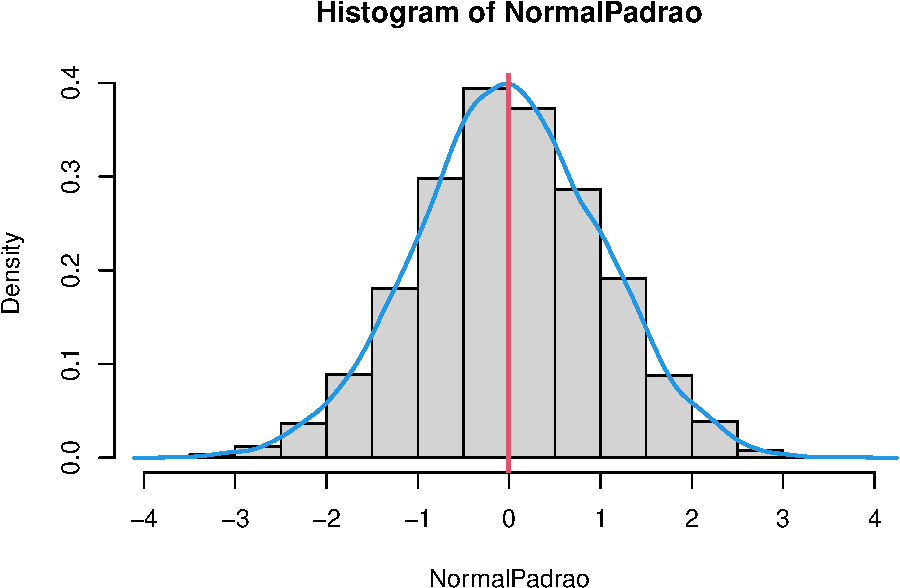
\includegraphics{Livro-Estatistica+R_files/figure-latex/unnamed-chunk-32-1.pdf}

No gráfico QQ, os quantis da amostra são comparados com os quantis da distribuição normal padrão. Se a amostra segue uma distribuição normal, os pontos no gráfico QQ devem se alinhar aproximadamente a uma linha reta.

Se os pontos se afastam dessa linha reta de forma sistemática, isso indica que os dados não seguem uma distribuição normal. O tipo de desvio pode dar pistas sobre a natureza dessa não-normalidade (por exemplo, se os pontos se curvam para cima ou para baixo, pode indicar assimetria ou caudas pesadas).

\begin{quote}
Distrbuição normal é usada para dados contínuos!
\end{quote}

\begin{Shaded}
\begin{Highlighting}[]
\CommentTok{\# Gráfico QQ}
\FunctionTok{set.seed}\NormalTok{(}\DecValTok{1}\NormalTok{)}
\NormalTok{BatimentosMulheres }\OtherTok{\textless{}{-}} \FunctionTok{rnorm}\NormalTok{(}\DecValTok{1000}\NormalTok{, }\DecValTok{70}\NormalTok{, }\DecValTok{3}\NormalTok{)}
\FunctionTok{qqnorm}\NormalTok{(BatimentosMulheres)}
\FunctionTok{qqline}\NormalTok{(BatimentosMulheres, }\AttributeTok{col=}\StringTok{"red"}\NormalTok{)}
\end{Highlighting}
\end{Shaded}

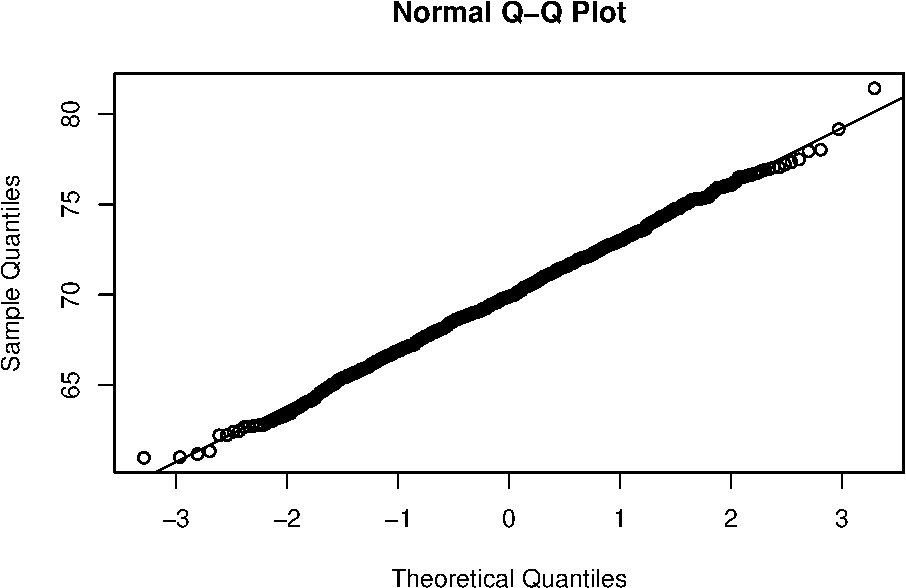
\includegraphics{Livro-Estatistica+R_files/figure-latex/unnamed-chunk-33-1.pdf}

\begin{Shaded}
\begin{Highlighting}[]
\CommentTok{\# Faça o arredondamento}
\NormalTok{BatimentosMulheresR }\OtherTok{\textless{}{-}} \FunctionTok{round}\NormalTok{(BatimentosMulheres,}\DecValTok{0}\NormalTok{)}
\FunctionTok{qqnorm}\NormalTok{(BatimentosMulheresR)}
\FunctionTok{qqline}\NormalTok{(BatimentosMulheresR)}
\end{Highlighting}
\end{Shaded}

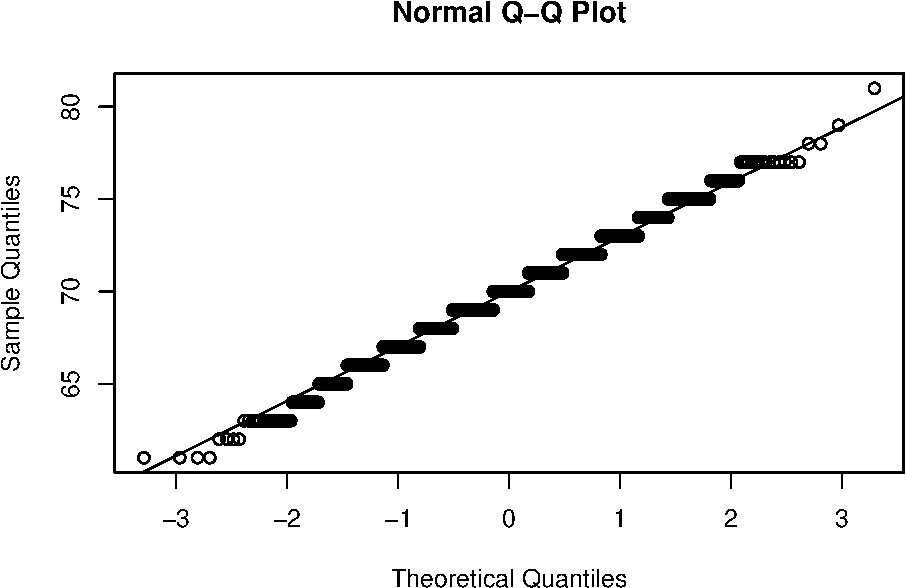
\includegraphics{Livro-Estatistica+R_files/figure-latex/unnamed-chunk-33-2.pdf}

\begin{quote}
A distribuição Normal é uma distribuição para modelar variáveis \textbf{CONTÍNUAS}!
\end{quote}

\section{Atividade 7}\label{atividade-7}

\textbf{Utilizando o banco de dados escolhido para as atividades 5 e 6, gere gráficos QQ para as variáveis quantitativas. Em seguida, avalie visualmente se essas variáveis seguem uma distribuição normal.}

\chapter{Exemplos de distribuições}\label{exemplos-de-distribuiuxe7uxf5es}

\section{Distribuições Discretas}\label{distribuiuxe7uxf5es-discretas}

\subsection{Binomial}\label{binomial}

Modela o número de sucessos em n tentativas com probabilidade \texttt{p}.

\begin{Shaded}
\begin{Highlighting}[]
\NormalTok{n }\OtherTok{\textless{}{-}} \DecValTok{10}
\NormalTok{p }\OtherTok{\textless{}{-}} \FloatTok{0.5}
\NormalTok{x }\OtherTok{\textless{}{-}} \DecValTok{0}\SpecialCharTok{:}\NormalTok{n}
\NormalTok{y }\OtherTok{\textless{}{-}} \FunctionTok{dbinom}\NormalTok{(x, }\AttributeTok{size =}\NormalTok{ n, }\AttributeTok{prob =}\NormalTok{ p)}

\FunctionTok{ggplot}\NormalTok{(}\FunctionTok{data.frame}\NormalTok{(x, y), }\FunctionTok{aes}\NormalTok{(x, y)) }\SpecialCharTok{+}
  \FunctionTok{geom\_bar}\NormalTok{(}\AttributeTok{stat =} \StringTok{"identity"}\NormalTok{, }\AttributeTok{fill =} \StringTok{"steelblue"}\NormalTok{) }\SpecialCharTok{+}
  \FunctionTok{labs}\NormalTok{(}\AttributeTok{title =} \StringTok{"Distribuição Binomial (n = 10, p = 0.5)"}\NormalTok{, }\AttributeTok{x =} \StringTok{"Número de Sucessos"}\NormalTok{, }\AttributeTok{y =} \StringTok{"Probabilidade"}\NormalTok{)}
\end{Highlighting}
\end{Shaded}

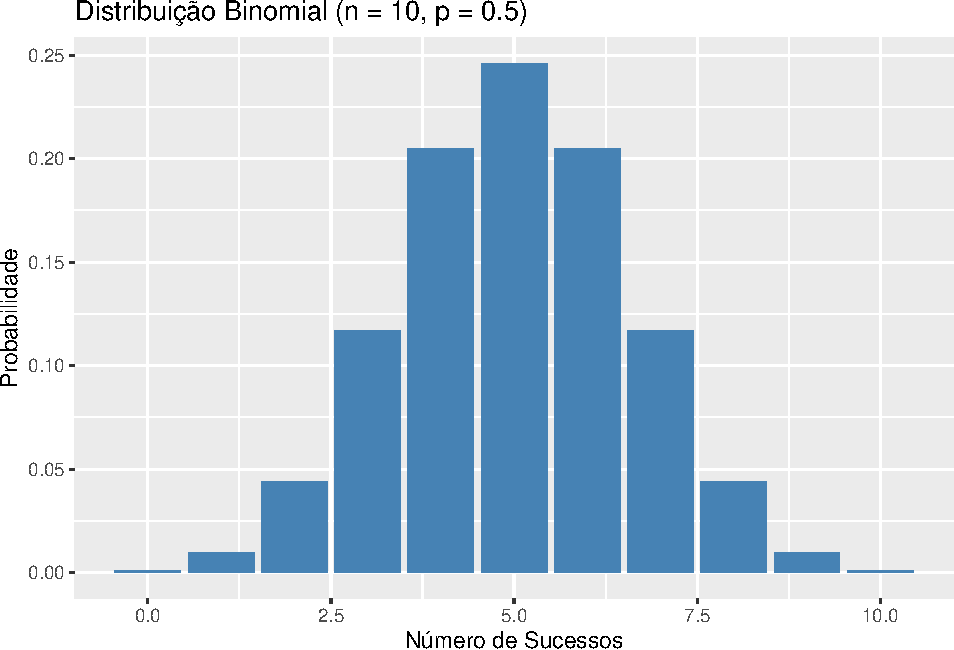
\includegraphics{Livro-Estatistica+R_files/figure-latex/binomial-1.pdf}

\subsection{Poisson}\label{poisson}

Modela o número de eventos raros num intervalo fixo.

\begin{Shaded}
\begin{Highlighting}[]
\NormalTok{lambda }\OtherTok{\textless{}{-}} \DecValTok{3}
\NormalTok{x }\OtherTok{\textless{}{-}} \DecValTok{0}\SpecialCharTok{:}\DecValTok{15}
\NormalTok{y }\OtherTok{\textless{}{-}} \FunctionTok{dpois}\NormalTok{(x, lambda)}

\FunctionTok{ggplot}\NormalTok{(}\FunctionTok{data.frame}\NormalTok{(x, y), }\FunctionTok{aes}\NormalTok{(x, y)) }\SpecialCharTok{+}
  \FunctionTok{geom\_bar}\NormalTok{(}\AttributeTok{stat =} \StringTok{"identity"}\NormalTok{, }\AttributeTok{fill =} \StringTok{"darkorange"}\NormalTok{) }\SpecialCharTok{+}
  \FunctionTok{labs}\NormalTok{(}\AttributeTok{title =} \StringTok{"Distribuição de Poisson (λ = 3)"}\NormalTok{, }\AttributeTok{x =} \StringTok{"Número de Eventos"}\NormalTok{, }\AttributeTok{y =} \StringTok{"Probabilidade"}\NormalTok{)}
\end{Highlighting}
\end{Shaded}

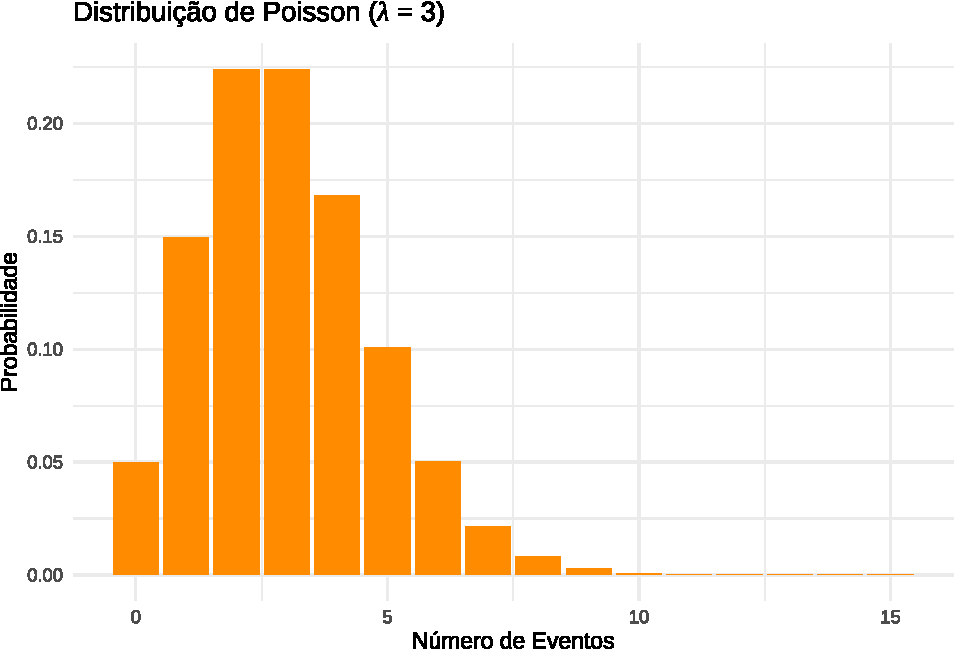
\includegraphics{Livro-Estatistica+R_files/figure-latex/poisson-1.pdf}

\subsection{Geométrica}\label{geomuxe9trica}

Modela o número de falhas antes do primeiro sucesso.

\begin{Shaded}
\begin{Highlighting}[]
\NormalTok{p }\OtherTok{\textless{}{-}} \FloatTok{0.3}
\NormalTok{x }\OtherTok{\textless{}{-}} \DecValTok{0}\SpecialCharTok{:}\DecValTok{10}
\NormalTok{y }\OtherTok{\textless{}{-}} \FunctionTok{dgeom}\NormalTok{(x, }\AttributeTok{prob =}\NormalTok{ p)}

\FunctionTok{ggplot}\NormalTok{(}\FunctionTok{data.frame}\NormalTok{(x, y), }\FunctionTok{aes}\NormalTok{(x, y)) }\SpecialCharTok{+}
  \FunctionTok{geom\_bar}\NormalTok{(}\AttributeTok{stat =} \StringTok{"identity"}\NormalTok{, }\AttributeTok{fill =} \StringTok{"purple"}\NormalTok{) }\SpecialCharTok{+}
  \FunctionTok{labs}\NormalTok{(}\AttributeTok{title =} \StringTok{"Distribuição Geométrica (p = 0.3)"}\NormalTok{, }\AttributeTok{x =} \StringTok{"Tentativas até o 1º Sucesso"}\NormalTok{, }\AttributeTok{y =} \StringTok{"Probabilidade"}\NormalTok{)}
\end{Highlighting}
\end{Shaded}

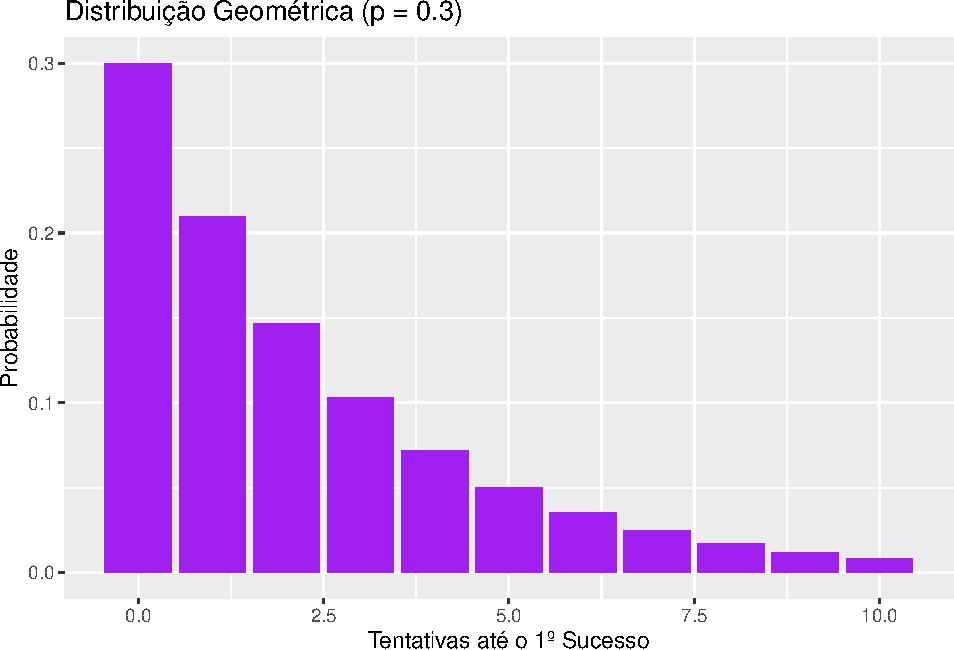
\includegraphics{Livro-Estatistica+R_files/figure-latex/geometrica-1.pdf}

\section{Distribuições Contínuas}\label{distribuiuxe7uxf5es-contuxednuas}

\subsection{Normal}\label{normal}

Modela fenômenos naturais e erros de medida.

\begin{Shaded}
\begin{Highlighting}[]
\NormalTok{x }\OtherTok{\textless{}{-}} \FunctionTok{seq}\NormalTok{(}\SpecialCharTok{{-}}\DecValTok{4}\NormalTok{, }\DecValTok{4}\NormalTok{, }\AttributeTok{length.out =} \DecValTok{100}\NormalTok{)}
\NormalTok{y }\OtherTok{\textless{}{-}} \FunctionTok{dnorm}\NormalTok{(x)}

\FunctionTok{ggplot}\NormalTok{(}\FunctionTok{data.frame}\NormalTok{(x, y), }\FunctionTok{aes}\NormalTok{(x, y)) }\SpecialCharTok{+}
  \FunctionTok{geom\_line}\NormalTok{(}\AttributeTok{color =} \StringTok{"darkgreen"}\NormalTok{, }\AttributeTok{linewidth =} \FloatTok{1.2}\NormalTok{) }\SpecialCharTok{+}
  \FunctionTok{labs}\NormalTok{(}\AttributeTok{title =} \StringTok{"Distribuição Normal (média = 0, sd = 1)"}\NormalTok{, }\AttributeTok{x =} \StringTok{"x"}\NormalTok{, }\AttributeTok{y =} \StringTok{"Densidade"}\NormalTok{)}
\end{Highlighting}
\end{Shaded}

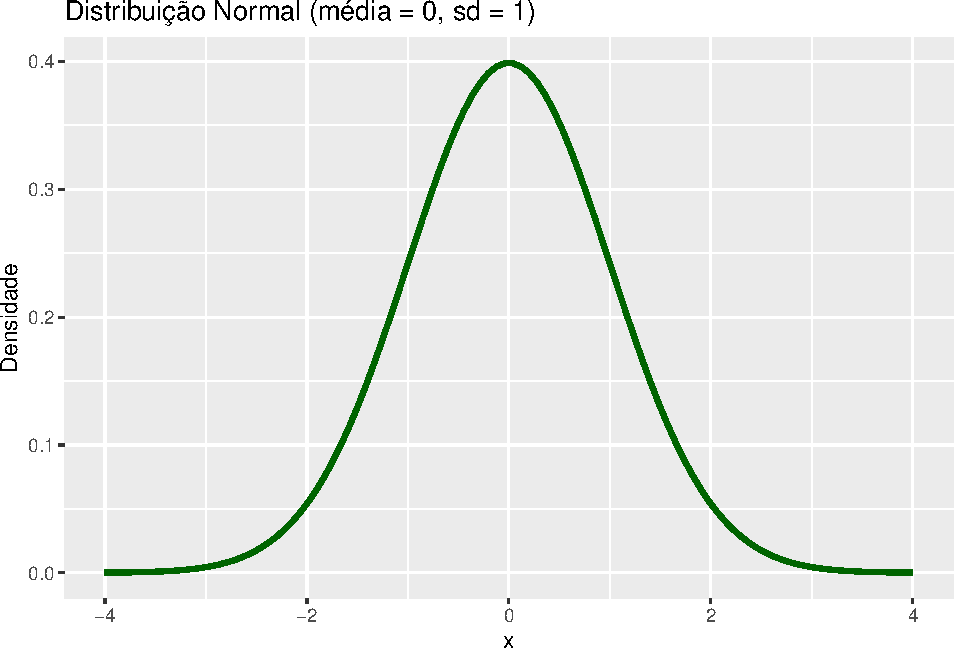
\includegraphics{Livro-Estatistica+R_files/figure-latex/normal_plot-1.pdf}

\subsection{Exponencial}\label{exponencial}

Tempo até um evento ocorrer.

\begin{Shaded}
\begin{Highlighting}[]
\NormalTok{lambda }\OtherTok{\textless{}{-}} \DecValTok{1}
\NormalTok{x }\OtherTok{\textless{}{-}} \FunctionTok{seq}\NormalTok{(}\DecValTok{0}\NormalTok{, }\DecValTok{5}\NormalTok{, }\AttributeTok{length.out =} \DecValTok{100}\NormalTok{)}
\NormalTok{y }\OtherTok{\textless{}{-}} \FunctionTok{dexp}\NormalTok{(x, }\AttributeTok{rate =}\NormalTok{ lambda)}

\FunctionTok{ggplot}\NormalTok{(}\FunctionTok{data.frame}\NormalTok{(x, y), }\FunctionTok{aes}\NormalTok{(x, y)) }\SpecialCharTok{+}
  \FunctionTok{geom\_line}\NormalTok{(}\AttributeTok{color =} \StringTok{"firebrick"}\NormalTok{, }\AttributeTok{size =} \FloatTok{1.2}\NormalTok{) }\SpecialCharTok{+}
  \FunctionTok{labs}\NormalTok{(}\AttributeTok{title =} \StringTok{"Distribuição Exponencial (λ = 1)"}\NormalTok{, }\AttributeTok{x =} \StringTok{"Tempo"}\NormalTok{, }\AttributeTok{y =} \StringTok{"Densidade"}\NormalTok{)}
\end{Highlighting}
\end{Shaded}

\begin{verbatim}
## Warning: Using `size` aesthetic for lines was deprecated in ggplot2 3.4.0.
## i Please use `linewidth` instead.
## This warning is displayed once every 8 hours.
## Call `lifecycle::last_lifecycle_warnings()` to see where this warning was
## generated.
\end{verbatim}

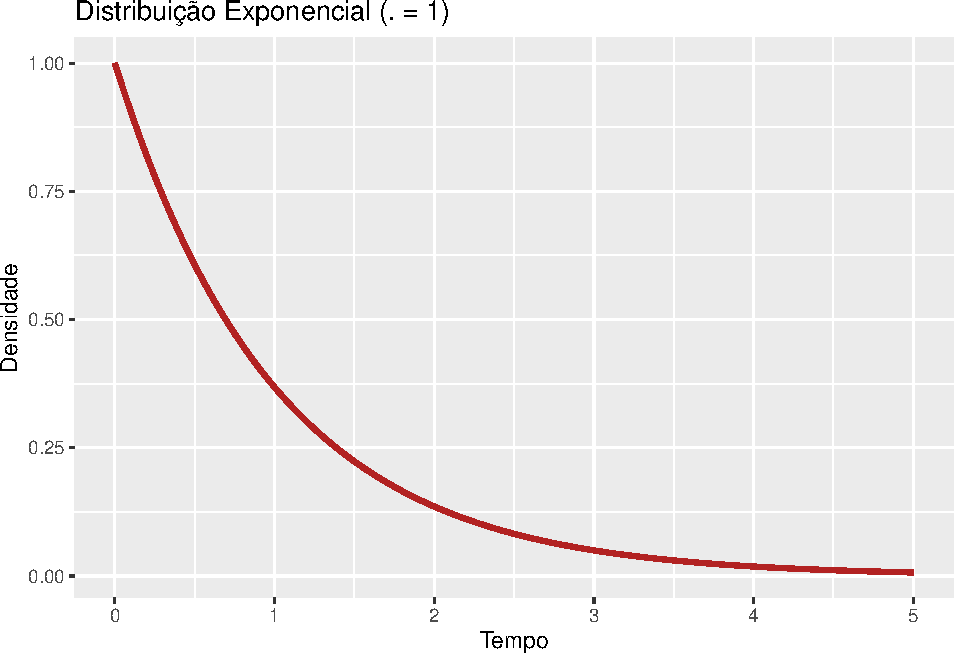
\includegraphics{Livro-Estatistica+R_files/figure-latex/exponencial-1.pdf}

\subsection{Uniforme Contínua}\label{uniforme-contuxednua}

Todos os valores têm a mesma chance.

\begin{Shaded}
\begin{Highlighting}[]
\NormalTok{x }\OtherTok{\textless{}{-}} \FunctionTok{seq}\NormalTok{(}\DecValTok{0}\NormalTok{, }\DecValTok{1}\NormalTok{, }\AttributeTok{length.out =} \DecValTok{100}\NormalTok{)}
\NormalTok{y }\OtherTok{\textless{}{-}} \FunctionTok{dunif}\NormalTok{(x, }\AttributeTok{min =} \DecValTok{0}\NormalTok{, }\AttributeTok{max =} \DecValTok{1}\NormalTok{)}

\FunctionTok{ggplot}\NormalTok{(}\FunctionTok{data.frame}\NormalTok{(x, y), }\FunctionTok{aes}\NormalTok{(x, y)) }\SpecialCharTok{+}
  \FunctionTok{geom\_line}\NormalTok{(}\AttributeTok{color =} \StringTok{"goldenrod"}\NormalTok{, }\AttributeTok{size =} \FloatTok{1.2}\NormalTok{) }\SpecialCharTok{+}
  \FunctionTok{labs}\NormalTok{(}\AttributeTok{title =} \StringTok{"Distribuição Uniforme Contínua (0 a 1)"}\NormalTok{, }\AttributeTok{x =} \StringTok{"x"}\NormalTok{, }\AttributeTok{y =} \StringTok{"Densidade"}\NormalTok{)}
\end{Highlighting}
\end{Shaded}

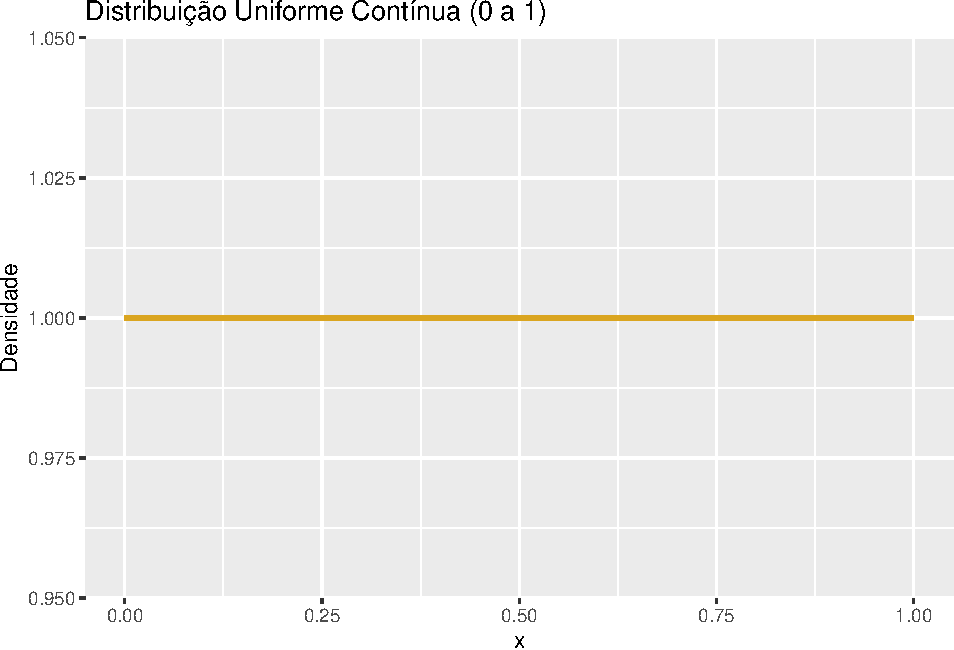
\includegraphics{Livro-Estatistica+R_files/figure-latex/uniforme-1.pdf}

\subsection{t de Student}\label{t-de-student}

Usada em testes com amostras pequenas.

\begin{Shaded}
\begin{Highlighting}[]
\NormalTok{x }\OtherTok{\textless{}{-}} \FunctionTok{seq}\NormalTok{(}\SpecialCharTok{{-}}\DecValTok{4}\NormalTok{, }\DecValTok{4}\NormalTok{, }\AttributeTok{length.out =} \DecValTok{100}\NormalTok{)}
\NormalTok{y }\OtherTok{\textless{}{-}} \FunctionTok{dt}\NormalTok{(x, }\AttributeTok{df =} \DecValTok{5}\NormalTok{)}

\FunctionTok{ggplot}\NormalTok{(}\FunctionTok{data.frame}\NormalTok{(x, y), }\FunctionTok{aes}\NormalTok{(x, y)) }\SpecialCharTok{+}
  \FunctionTok{geom\_line}\NormalTok{(}\AttributeTok{color =} \StringTok{"navy"}\NormalTok{, }\AttributeTok{size =} \FloatTok{1.2}\NormalTok{) }\SpecialCharTok{+}
  \FunctionTok{labs}\NormalTok{(}\AttributeTok{title =} \StringTok{"Distribuição t de Student (df = 5)"}\NormalTok{, }\AttributeTok{x =} \StringTok{"x"}\NormalTok{, }\AttributeTok{y =} \StringTok{"Densidade"}\NormalTok{)}
\end{Highlighting}
\end{Shaded}

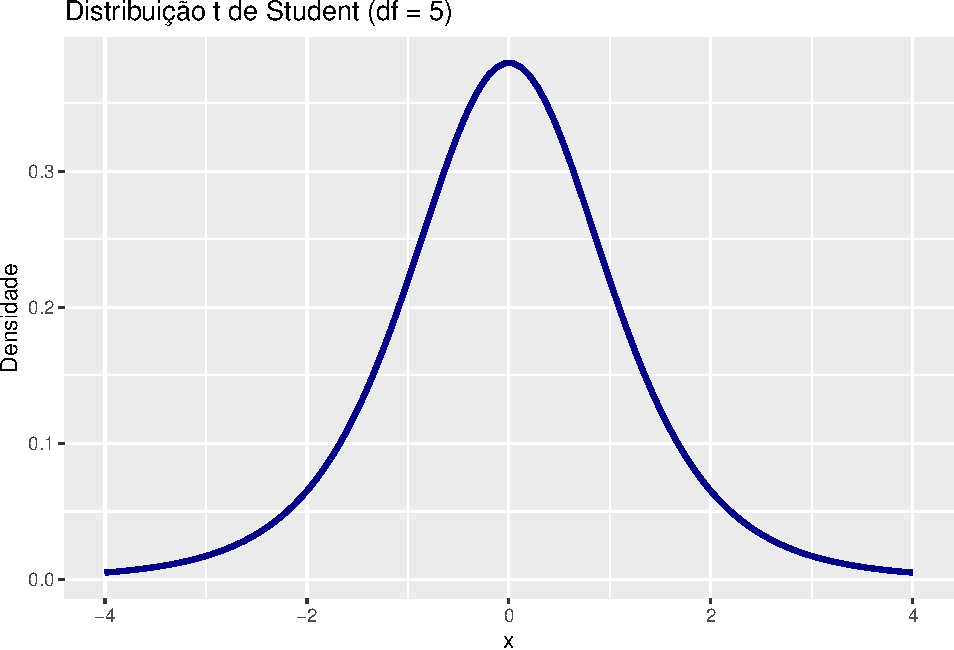
\includegraphics{Livro-Estatistica+R_files/figure-latex/student-1.pdf}

\subsection{Qui-Quadrado (χ²)}\label{qui-quadrado-ux3c7uxb2}

Usada para testes de aderência e independência.

\begin{Shaded}
\begin{Highlighting}[]
\NormalTok{x }\OtherTok{\textless{}{-}} \FunctionTok{seq}\NormalTok{(}\DecValTok{0}\NormalTok{, }\DecValTok{20}\NormalTok{, }\AttributeTok{length.out =} \DecValTok{100}\NormalTok{)}
\NormalTok{y }\OtherTok{\textless{}{-}} \FunctionTok{dchisq}\NormalTok{(x, }\AttributeTok{df =} \DecValTok{5}\NormalTok{)}

\FunctionTok{ggplot}\NormalTok{(}\FunctionTok{data.frame}\NormalTok{(x, y), }\FunctionTok{aes}\NormalTok{(x, y)) }\SpecialCharTok{+}
  \FunctionTok{geom\_line}\NormalTok{(}\AttributeTok{color =} \StringTok{"tomato"}\NormalTok{, }\AttributeTok{size =} \FloatTok{1.2}\NormalTok{) }\SpecialCharTok{+}
  \FunctionTok{labs}\NormalTok{(}\AttributeTok{title =} \StringTok{"Distribuição Qui{-}quadrado (df = 5)"}\NormalTok{, }\AttributeTok{x =} \StringTok{"x"}\NormalTok{, }\AttributeTok{y =} \StringTok{"Densidade"}\NormalTok{)}
\end{Highlighting}
\end{Shaded}

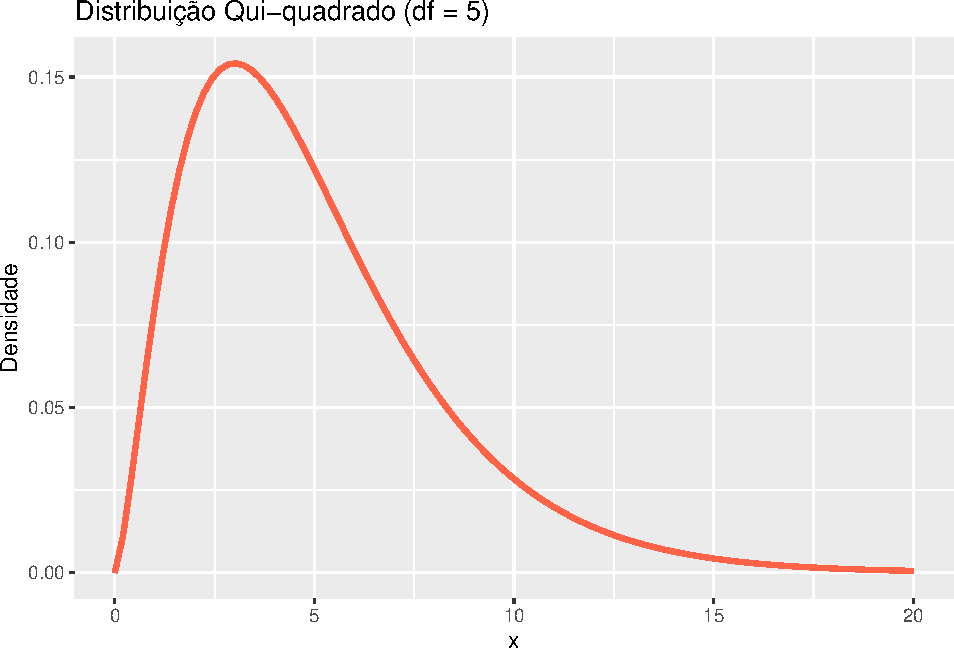
\includegraphics{Livro-Estatistica+R_files/figure-latex/chisq-1.pdf}

\subsection{F de Fisher}\label{f-de-fisher}

Usada em ANOVA para comparar variâncias.

\begin{Shaded}
\begin{Highlighting}[]
\NormalTok{x }\OtherTok{\textless{}{-}} \FunctionTok{seq}\NormalTok{(}\DecValTok{0}\NormalTok{, }\DecValTok{5}\NormalTok{, }\AttributeTok{length.out =} \DecValTok{100}\NormalTok{)}
\NormalTok{y }\OtherTok{\textless{}{-}} \FunctionTok{df}\NormalTok{(x, }\AttributeTok{df1 =} \DecValTok{5}\NormalTok{, }\AttributeTok{df2 =} \DecValTok{10}\NormalTok{)}

\FunctionTok{ggplot}\NormalTok{(}\FunctionTok{data.frame}\NormalTok{(x, y), }\FunctionTok{aes}\NormalTok{(x, y)) }\SpecialCharTok{+}
  \FunctionTok{geom\_line}\NormalTok{(}\AttributeTok{color =} \StringTok{"darkviolet"}\NormalTok{, }\AttributeTok{size =} \FloatTok{1.2}\NormalTok{) }\SpecialCharTok{+}
  \FunctionTok{labs}\NormalTok{(}\AttributeTok{title =} \StringTok{"Distribuição F de Fisher (df1 = 5, df2 = 10)"}\NormalTok{, }\AttributeTok{x =} \StringTok{"x"}\NormalTok{, }\AttributeTok{y =} \StringTok{"Densidade"}\NormalTok{)}
\end{Highlighting}
\end{Shaded}

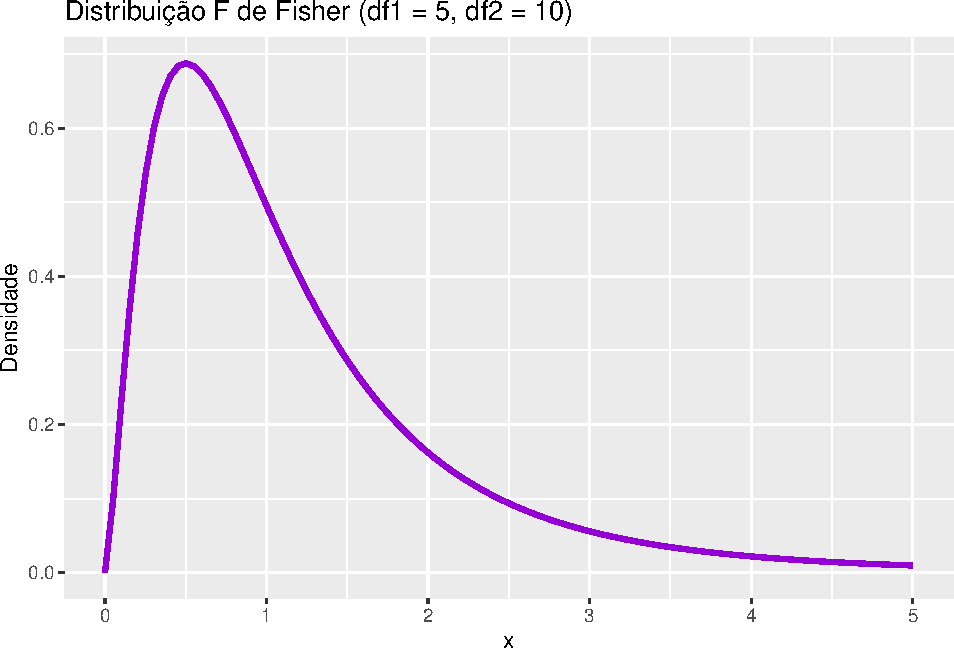
\includegraphics{Livro-Estatistica+R_files/figure-latex/fisher-1.pdf}

\begin{quote}
Cada distribuição tem uma aplicação específica conforme o tipo de variável (discreta ou contínua), o contexto do problema e as suposições do modelo. Entender suas formas e usos ajuda na escolha correta da análise estatística.
\end{quote}

\chapter{Normal ou Não?}\label{normal-ou-nuxe3o}

Antes de avançarmos para a aplicação dos testes estatísticos, é importante avaliarmos se os dados seguem ou não uma distribuição normal. Essa verificação inicial é muito importante porque muitos testes paramétricos, como o teste t e a ANOVA, partem da suposição de normalidade dos dados. Compreender esse aspecto permite escolher os métodos estatísticos mais adequados, aumentando a confiabilidade dos resultados e evitando interpretações equivocadas que poderiam comprometer a análise.

Esta seção apresenta uma análise visual da normalidade dos dados por meio de gráficos QQ (Quantil-Quantil), com a comparação de três cenários distintos: dados que seguem uma distribuição normal, dados que levantam dúvidas quanto à normalidade e dados que claramente não seguem essa distribuição.

\begin{itemize}
\tightlist
\item
  Dados normalmente distribuídos
\item
  Dados que geram dúvida quanto à normalidade
\item
  Dados que claramente não seguem distribuição normal
\end{itemize}

\section{Dados que seguem distribuição normal}\label{dados-que-seguem-distribuiuxe7uxe3o-normal}

\begin{Shaded}
\begin{Highlighting}[]
\FunctionTok{set.seed}\NormalTok{(}\DecValTok{10}\NormalTok{)}
\NormalTok{dados\_normais }\OtherTok{\textless{}{-}} \FunctionTok{rnorm}\NormalTok{(}\DecValTok{500}\NormalTok{, }\AttributeTok{mean =} \DecValTok{0}\NormalTok{, }\AttributeTok{sd =} \DecValTok{1}\NormalTok{)}

\FunctionTok{hist}\NormalTok{(dados\_normais, }\AttributeTok{main =} \StringTok{"Histograma {-} Distribuição Normal"}\NormalTok{, }\AttributeTok{col =} \StringTok{"lightblue"}\NormalTok{)}
\end{Highlighting}
\end{Shaded}

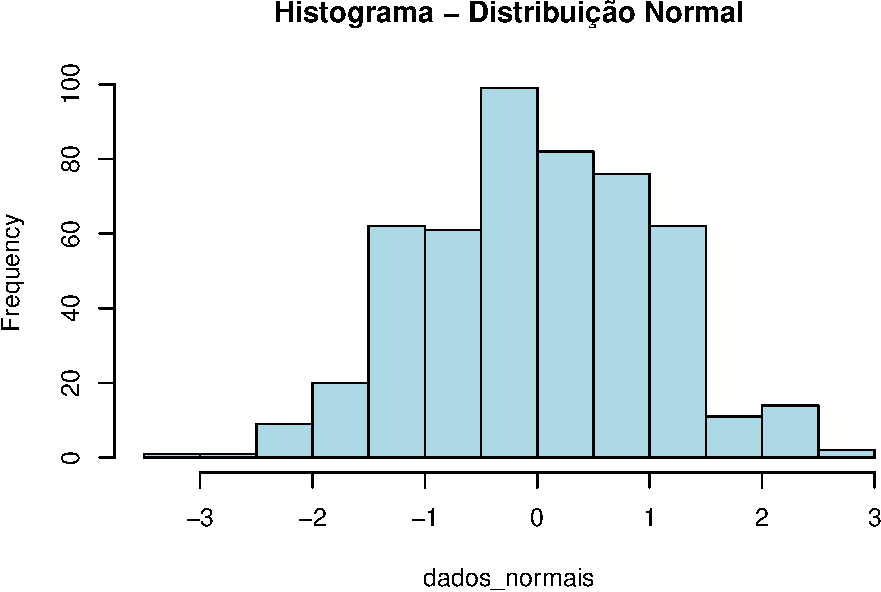
\includegraphics{Livro-Estatistica+R_files/figure-latex/enormal-1.pdf}

\begin{Shaded}
\begin{Highlighting}[]
\FunctionTok{boxplot}\NormalTok{(dados\_normais, }\AttributeTok{main =} \StringTok{"Boxplot {-} Distribuição Normal"}\NormalTok{)}
\end{Highlighting}
\end{Shaded}

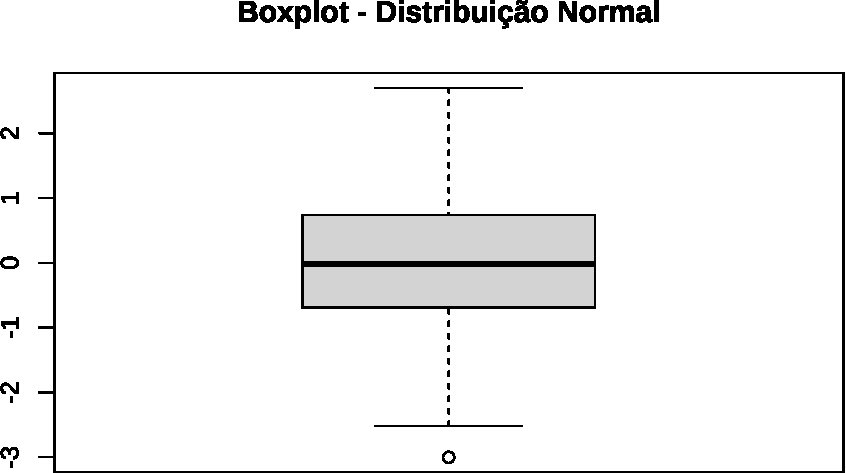
\includegraphics{Livro-Estatistica+R_files/figure-latex/enormal-2.pdf}

\begin{Shaded}
\begin{Highlighting}[]
\FunctionTok{qqnorm}\NormalTok{(dados\_normais, }\AttributeTok{main =} \StringTok{"QQ Plot {-} Distribuição Normal"}\NormalTok{)}
\FunctionTok{qqline}\NormalTok{(dados\_normais, }\AttributeTok{col =} \StringTok{"blue"}\NormalTok{, }\AttributeTok{lwd =} \DecValTok{2}\NormalTok{)}
\end{Highlighting}
\end{Shaded}

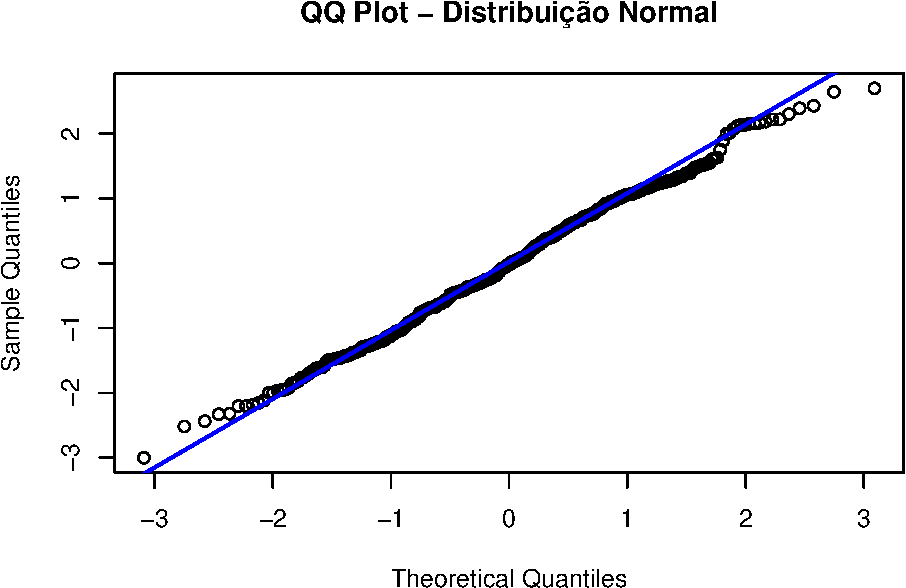
\includegraphics{Livro-Estatistica+R_files/figure-latex/enormal-3.pdf}

\emph{Observação:} Os pontos seguem de perto a linha, indicando que os dados são normalmente distribuídos.

\section{Dados que geram dúvida}\label{dados-que-geram-duxfavida}

\begin{Shaded}
\begin{Highlighting}[]
\FunctionTok{set.seed}\NormalTok{(}\DecValTok{20}\NormalTok{)}
\NormalTok{dados\_mistos }\OtherTok{\textless{}{-}} \FunctionTok{c}\NormalTok{(}\FunctionTok{rnorm}\NormalTok{(}\DecValTok{250}\NormalTok{, }\DecValTok{0}\NormalTok{, }\DecValTok{1}\NormalTok{), }\FunctionTok{rnorm}\NormalTok{(}\DecValTok{250}\NormalTok{, }\DecValTok{2}\NormalTok{, }\DecValTok{1}\NormalTok{))}

\FunctionTok{hist}\NormalTok{(dados\_mistos, }\AttributeTok{main =} \StringTok{"Histograma {-} Mistura de Normais"}\NormalTok{, }\AttributeTok{col =} \StringTok{"lightgreen"}\NormalTok{)}
\end{Highlighting}
\end{Shaded}

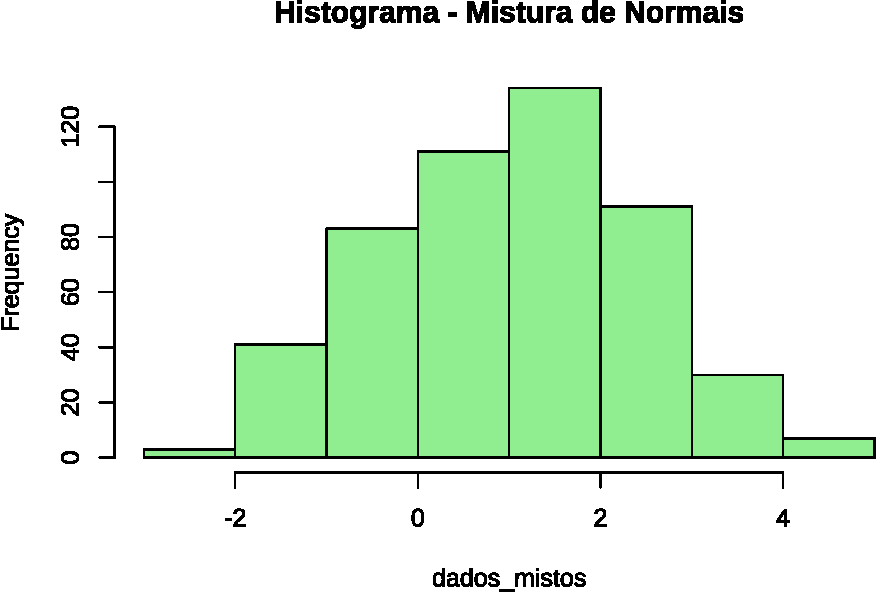
\includegraphics{Livro-Estatistica+R_files/figure-latex/duvidosa-1.pdf}

\begin{Shaded}
\begin{Highlighting}[]
\FunctionTok{boxplot}\NormalTok{(dados\_mistos, }\AttributeTok{main =} \StringTok{"Boxplot {-} Mistura de Normais"}\NormalTok{)}
\end{Highlighting}
\end{Shaded}

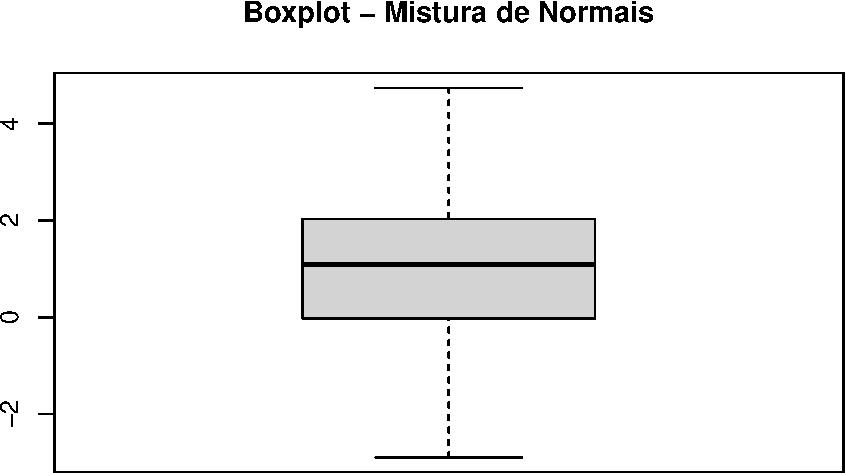
\includegraphics{Livro-Estatistica+R_files/figure-latex/duvidosa-2.pdf}

\begin{Shaded}
\begin{Highlighting}[]
\FunctionTok{qqnorm}\NormalTok{(dados\_mistos, }\AttributeTok{main =} \StringTok{"QQ Plot {-} Mistura de Normais"}\NormalTok{)}
\FunctionTok{qqline}\NormalTok{(dados\_mistos, }\AttributeTok{col =} \StringTok{"orange"}\NormalTok{, }\AttributeTok{lwd =} \DecValTok{2}\NormalTok{)}
\end{Highlighting}
\end{Shaded}

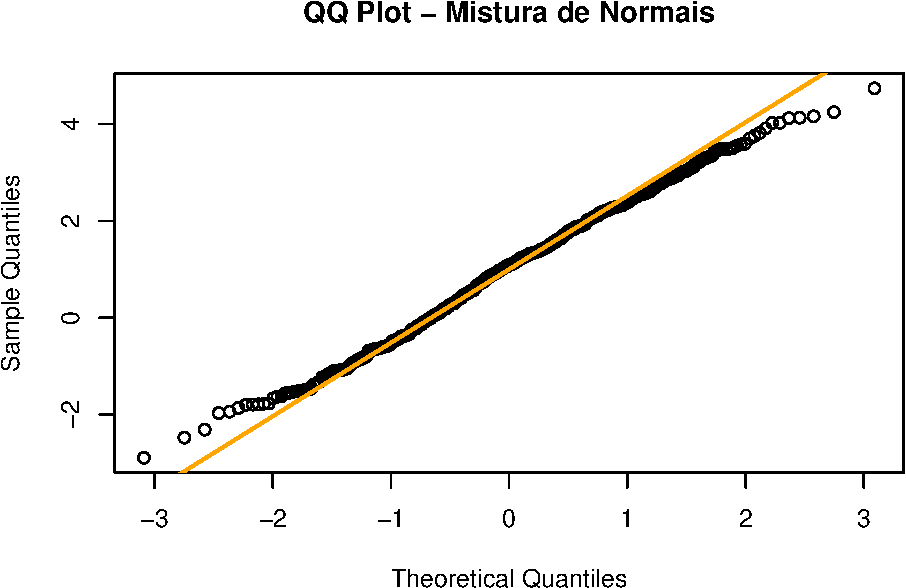
\includegraphics{Livro-Estatistica+R_files/figure-latex/duvidosa-3.pdf}

\emph{Observação:} As caudas do gráfico QQ começam a se afastar da linha, o que pode gerar dúvida sobre a normalidade.

\section{Dados que não seguem distribuição normal}\label{dados-que-nuxe3o-seguem-distribuiuxe7uxe3o-normal}

\begin{Shaded}
\begin{Highlighting}[]
\FunctionTok{set.seed}\NormalTok{(}\DecValTok{30}\NormalTok{)}
\NormalTok{dados\_chi }\OtherTok{\textless{}{-}} \FunctionTok{rchisq}\NormalTok{(}\DecValTok{500}\NormalTok{, }\AttributeTok{df =} \DecValTok{3}\NormalTok{)}

\FunctionTok{hist}\NormalTok{(dados\_chi, }\AttributeTok{main =} \StringTok{"Histograma {-} Distribuição Qui{-}quadrado"}\NormalTok{, }\AttributeTok{col =} \StringTok{"lightpink"}\NormalTok{)}
\end{Highlighting}
\end{Shaded}

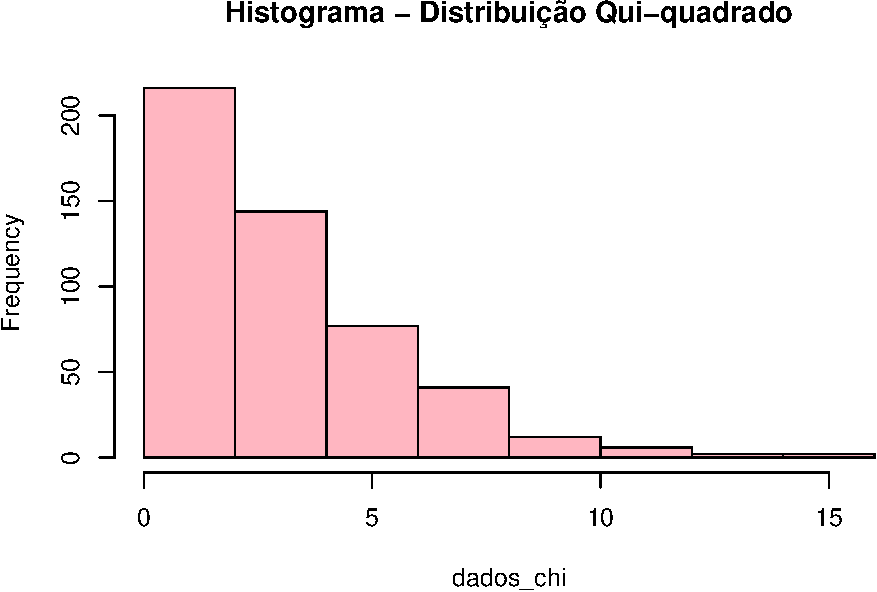
\includegraphics{Livro-Estatistica+R_files/figure-latex/nnormal-1.pdf}

\begin{Shaded}
\begin{Highlighting}[]
\FunctionTok{boxplot}\NormalTok{(dados\_chi, }\AttributeTok{main =} \StringTok{"Boxplot {-} Qui{-}quadrado"}\NormalTok{)}
\end{Highlighting}
\end{Shaded}

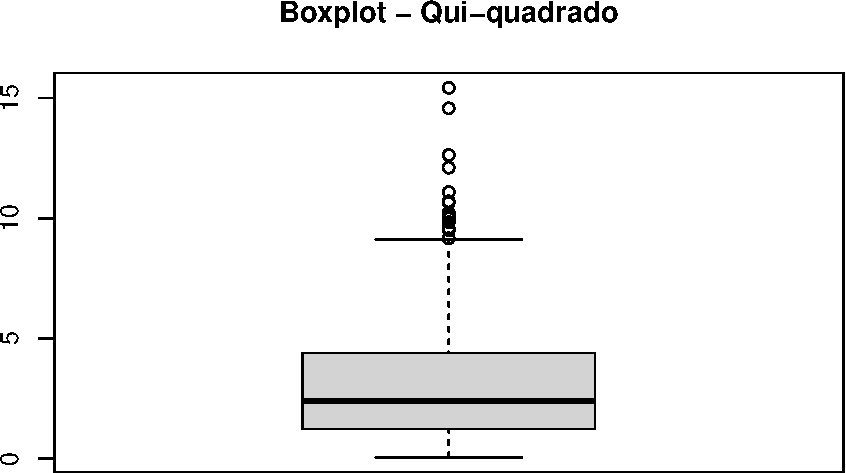
\includegraphics{Livro-Estatistica+R_files/figure-latex/nnormal-2.pdf}

\begin{Shaded}
\begin{Highlighting}[]
\FunctionTok{qqnorm}\NormalTok{(dados\_chi, }\AttributeTok{main =} \StringTok{"QQ Plot {-} Qui{-}quadrado"}\NormalTok{)}
\FunctionTok{qqline}\NormalTok{(dados\_chi, }\AttributeTok{col =} \StringTok{"red"}\NormalTok{, }\AttributeTok{lwd =} \DecValTok{2}\NormalTok{)}
\end{Highlighting}
\end{Shaded}

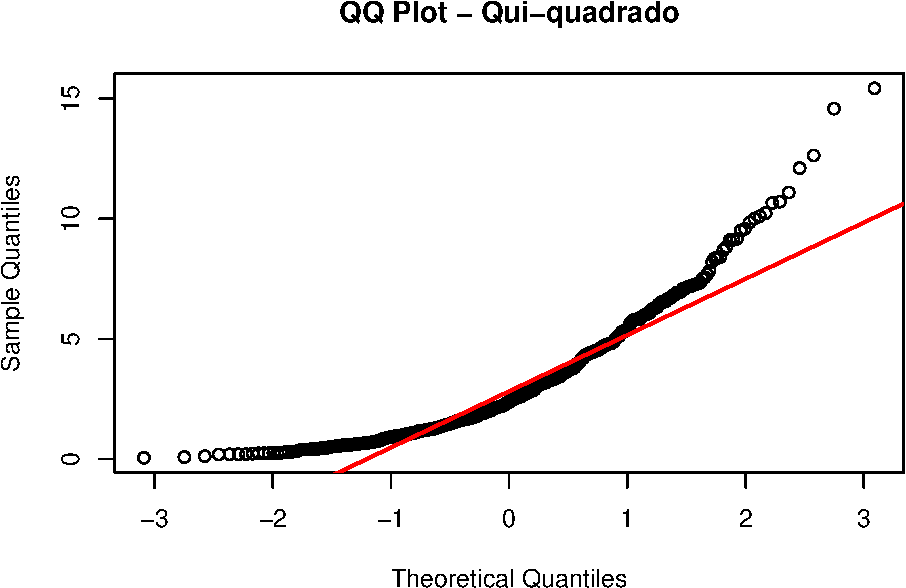
\includegraphics{Livro-Estatistica+R_files/figure-latex/nnormal-3.pdf}

\emph{Observação:} A forte curvatura do gráfico QQ indica clara violação da normalidade (assimetria à direita).

\section{Dados com forte concentração de repetição de valor (não seguem distribuição normal)}\label{dados-com-forte-concentrauxe7uxe3o-de-repetiuxe7uxe3o-de-valor-nuxe3o-seguem-distribuiuxe7uxe3o-normal}

\begin{Shaded}
\begin{Highlighting}[]
\FunctionTok{set.seed}\NormalTok{(}\DecValTok{42}\NormalTok{)}
\NormalTok{dados\_repetidos }\OtherTok{\textless{}{-}} \FunctionTok{c}\NormalTok{(}\FunctionTok{rep}\NormalTok{(}\DecValTok{18}\NormalTok{, }\DecValTok{5}\NormalTok{), }\FunctionTok{rep}\NormalTok{(}\DecValTok{23}\NormalTok{, }\DecValTok{10}\NormalTok{), }\FunctionTok{rep}\NormalTok{(}\DecValTok{26}\NormalTok{,}\DecValTok{7}\NormalTok{)) }

\CommentTok{\# Histograma}
\FunctionTok{hist}\NormalTok{(dados\_repetidos, }\AttributeTok{main =} \StringTok{"Histograma {-} Dados Repetidos"}\NormalTok{, }\AttributeTok{col =} \StringTok{"lightblue"}\NormalTok{, }\AttributeTok{xlab =} \StringTok{"Valor"}\NormalTok{, }\AttributeTok{ylab =} \StringTok{"Frequência"}\NormalTok{)}
\end{Highlighting}
\end{Shaded}

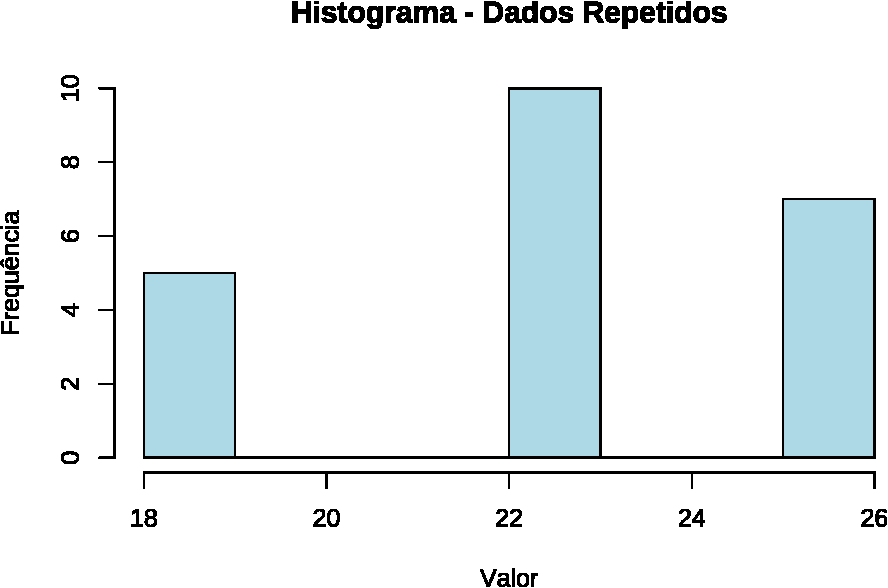
\includegraphics{Livro-Estatistica+R_files/figure-latex/dados_repetidos-1.pdf}

\begin{Shaded}
\begin{Highlighting}[]
\CommentTok{\# Boxplot}
\FunctionTok{boxplot}\NormalTok{(dados\_repetidos, }\AttributeTok{main =} \StringTok{"Boxplot {-} Dados Repetidos"}\NormalTok{, }\AttributeTok{col =} \StringTok{"lightgreen"}\NormalTok{)}
\end{Highlighting}
\end{Shaded}

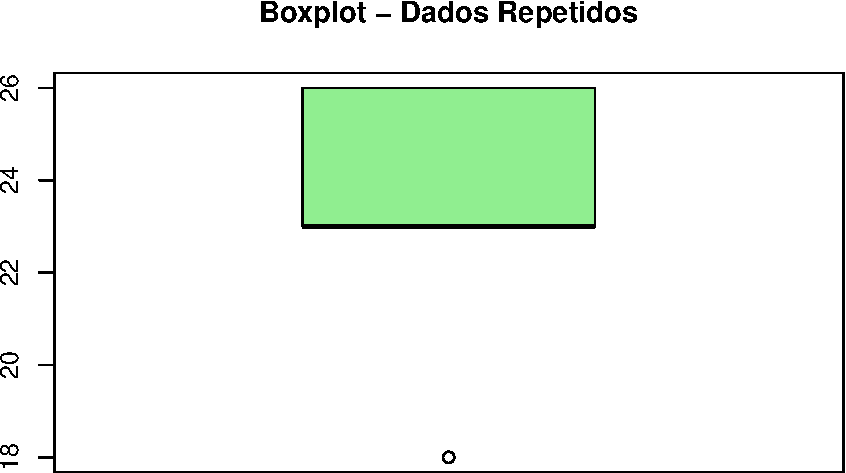
\includegraphics{Livro-Estatistica+R_files/figure-latex/dados_repetidos-2.pdf}

\begin{Shaded}
\begin{Highlighting}[]
\CommentTok{\# QQ Plot}
\FunctionTok{qqnorm}\NormalTok{(dados\_repetidos, }\AttributeTok{main =} \StringTok{"QQ Plot {-} Dados Repetidos"}\NormalTok{)}
\FunctionTok{qqline}\NormalTok{(dados\_repetidos, }\AttributeTok{col =} \StringTok{"red"}\NormalTok{, }\AttributeTok{lwd =} \DecValTok{2}\NormalTok{)}
\end{Highlighting}
\end{Shaded}

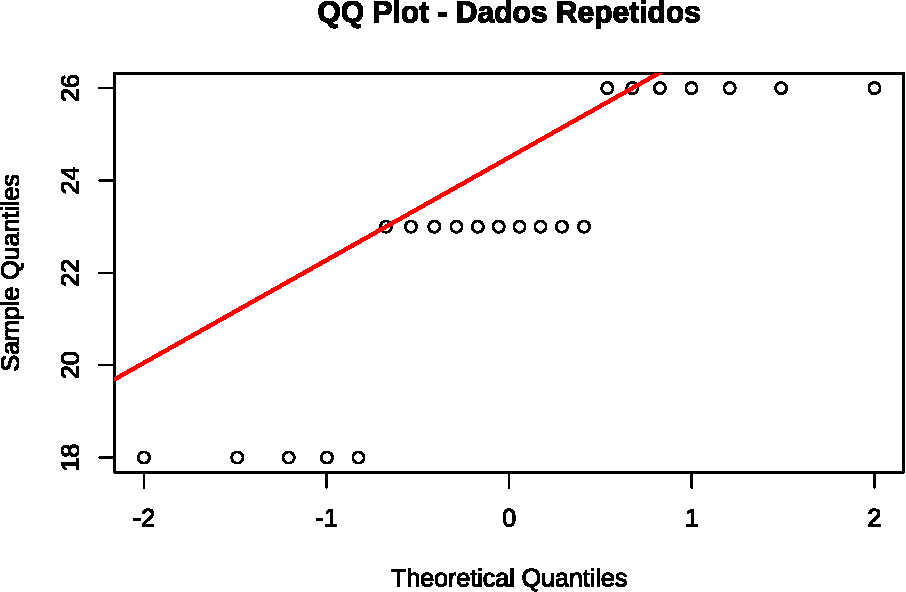
\includegraphics{Livro-Estatistica+R_files/figure-latex/dados_repetidos-3.pdf}

\begin{quote}
O gráfico QQ é uma ferramenta visual poderosa para avaliar se um conjunto de dados segue uma distribuição normal. Em conjunto com histogramas e boxplots, permite identificar desvios, outliers e assimetrias de maneira clara.
\end{quote}

\chapter{Estatística Inferencial}\label{estatuxedstica-inferencial-2}

A \textbf{estatística inferencial} é uma área essencial da estatística que permite fazer generalizações sobre uma população com base em dados coletados de uma amostra. Um passo fundamental nesse processo é o \textbf{cálculo amostral}, que determina o tamanho ideal da amostra para garantir a validade dos resultados --- e esse cálculo depende diretamente do \textbf{tipo de teste estatístico} que será utilizado, pois diferentes testes exigem diferentes parâmetros, como variabilidade, efeito esperado e poder do teste.

Ao conduzir uma análise inferencial, formulam-se \textbf{hipóteses}: a \textbf{hipótese nula (H₀)}, que representa a ausência de efeito ou diferença, e a \textbf{hipótese alternativa (H₁)}, que sugere a existência de um efeito ou diferença. Define-se também um \textbf{nível de significância (α)}, geralmente 0,05 (5\%), que representa a probabilidade de rejeitar H₀ quando ela é verdadeira (\textbf{erro tipo I}). O \textbf{valor-p}, calculado a partir dos dados, indica a probabilidade de obter um resultado tão extremo quanto o observado, supondo que H₀ seja verdadeira. Com base na comparação entre o valor-p e o nível de significância, aplica-se o \textbf{critério de decisão}: se o valor-p for menor que α, rejeita-se H₀, o que indica \textbf{evidências estatísticas suficientes para apoiar a hipótese alternativa}.

\section{Etapas de um Teste Estatístico}\label{etapas-de-um-teste-estatuxedstico}

Para realizar qualquer \textbf{teste estatístico}, seguimos uma sequência básica de passos:

\begin{enumerate}
\def\labelenumi{\arabic{enumi}.}
\item
  \textbf{Escrevemos as hipóteses do teste}, começando com a \textbf{hipótese nula (H₀)}, que geralmente afirma que não há efeito ou diferença, e a \textbf{hipótese alternativa (H₁)}, que propõe o contrário.
\item
  \textbf{Definimos o nível de significância (α)}, que é a margem de erro aceitável. Esse valor, geralmente 0,05 (ou 5\%), já foi considerado no \textbf{cálculo do tamanho da amostra}, garantindo que os resultados tenham confiabilidade.
\item
  \textbf{Utilizamos um recurso computacional}, como um software estatístico, para calcular o \textbf{valor-p}, que mostra a probabilidade de observarmos os dados coletados caso a hipótese nula seja verdadeira.
\item
  \textbf{Comparamos o valor-p com o nível de significância}. Se o valor-p for menor que α, \textbf{rejeitamos a hipótese nula}. Caso contrário, não rejeitamos.
\item
  Por fim, \textbf{chegamos à conclusão do teste}, que nos diz se há ou não \textbf{evidência estatística} suficiente para apoiar a hipótese alternativa.
\end{enumerate}

\section{Erros Tipo I e Tipo II}\label{erros-tipo-i-e-tipo-ii}

Em um \textbf{teste estatístico}, tomamos uma decisão com base nos dados coletados de uma amostra: \textbf{rejeitar} ou \textbf{não rejeitar a hipótese nula (H₀)}. Por isso, é fundamental realizar um \textbf{cálculo amostral adequado}, selecionar cuidadosamente a \textbf{técnica de amostragem} e estar atento às possíveis \textbf{fontes de vieses}, garantindo que a amostra seja representativa e que os resultados do teste sejam confiáveis.

Entretanto, essa decisão envolve \textbf{riscos de erro}, que são inerentes ao processo justamente porque estamos baseando nossas conclusões em uma amostra e não na população inteira. Esses erros se dividem em dois tipos:

\begin{itemize}
\item
  \textbf{Erro Tipo I (α) -- Falso Positivo}\\
  Ocorre quando \textbf{rejeitamos H₀ mesmo ela sendo verdadeira}.\\
  É como afirmar que existe um efeito quando, na verdade, não existe.

  \begin{quote}
  Exemplo na medicina: concluir que um novo medicamento reduz a pressão arterial quando ele não tem efeito real, o que pode levar à aprovação de um tratamento ineficaz.
  \end{quote}

  \begin{quote}
  Exemplo no esporte: afirmar que um programa de treinamento melhora o desempenho dos atletas quando ele não traz benefício real, gerando investimentos desnecessários.
  \end{quote}

  \begin{quote}
  Exemplo na psicologia: dizer que uma terapia cognitivo-comportamental reduz a ansiedade, mesmo sem efeito comprovado, gerando falsas expectativas nos pacientes.
  \end{quote}

  Essa é a chance de um \textbf{falso positivo}, e o \textbf{nível de significância α} (geralmente 0,05) representa a probabilidade de cometer esse erro.
\item
  \textbf{Erro Tipo II (β) -- Falso Negativo}\\
  Ocorre quando \textbf{não rejeitamos H₀ mesmo ela sendo falsa}.\\
  É como deixar passar um efeito real sem detectá-lo.

  \begin{quote}
  Exemplo na medicina: não identificar que o medicamento é eficaz, rejeitando seu uso quando ele realmente funciona.
  \end{quote}

  \begin{quote}
  Exemplo no esporte: não perceber a melhora no desempenho causada pelo programa de treinamento, deixando de adotá-lo e prejudicando os atletas.
  \end{quote}

  \begin{quote}
  Exemplo na psicologia: não detectar que a terapia é eficaz para reduzir a ansiedade, levando à rejeição de um tratamento que poderia beneficiar os pacientes.
  \end{quote}

  Isso é um \textbf{falso negativo}, e \textbf{β} é a probabilidade de cometer esse erro.
\end{itemize}

\section{Poder do Teste Estatístico}\label{poder-do-teste-estatuxedstico}

\begin{itemize}
\tightlist
\item
  O \textbf{poder do teste} é a probabilidade de \textbf{detectar um efeito real quando ele realmente existe}, ou seja, \textbf{rejeitar H₀ quando H₀ é falsa}.\\
\item
  O poder é calculado como:\\
  \textbf{Poder = 1 - β}
\end{itemize}

Um teste com \textbf{alto poder} (geralmente desejado acima de 80\%) tem menos chance de cometer erro tipo II, o que significa maior capacidade de detectar diferenças reais quando elas existem. O poder depende do \textbf{tamanho da amostra}, do \textbf{nível de significância}, da \textbf{variabilidade dos dados} e da \textbf{magnitude do efeito} que se deseja identificar.

\section{Tabela: Erros, Decisões e Poder do Teste}\label{tabela-erros-decisuxf5es-e-poder-do-teste}

\begin{longtable}[]{@{}
  >{\centering\arraybackslash}p{(\columnwidth - 4\tabcolsep) * \real{0.2414}}
  >{\centering\arraybackslash}p{(\columnwidth - 4\tabcolsep) * \real{0.3678}}
  >{\centering\arraybackslash}p{(\columnwidth - 4\tabcolsep) * \real{0.3908}}@{}}
\toprule\noalign{}
\begin{minipage}[b]{\linewidth}\centering
Situação Real
\end{minipage} & \begin{minipage}[b]{\linewidth}\centering
Decisão: Rejeitar H₀
\end{minipage} & \begin{minipage}[b]{\linewidth}\centering
Decisão: Não Rejeitar H₀
\end{minipage} \\
\midrule\noalign{}
\endhead
\bottomrule\noalign{}
\endlastfoot
H₀ é verdadeira & Erro Tipo I (\emph{α}) & Decisão correta \\
H₀ é falsa & Decisão correta (\emph{poder}) & Erro Tipo II (\emph{β}) \\
\end{longtable}

\begin{itemize}
\tightlist
\item
  \textbf{Poder do teste:} Probabilidade de rejeitar H₀ quando H₀ é falsa (ou seja, evitar o erro tipo II).
\end{itemize}

\section{Tamanho do Efeito}\label{tamanho-do-efeito}

\subsection{O que é o Tamanho do Efeito?}\label{o-que-uxe9-o-tamanho-do-efeito}

O \textbf{tamanho do efeito} é uma medida que indica \textbf{o quanto uma diferença ou relação observada nos dados é relevante na prática}.

Enquanto o \textbf{valor-p} nos informa se um resultado é estatisticamente significativo (ou seja, se é improvável que tenha ocorrido por acaso), o tamanho do efeito \textbf{complementa essa análise mostrando a magnitude real do efeito observado}.

\subsection{Exemplos para Entender Melhor}\label{exemplos-para-entender-melhor}

\begin{quote}
Imagine que um novo remédio reduza a pressão arterial em média em \textbf{1 mmHg} comparado ao tratamento padrão.\\
Com uma amostra muito grande, essa pequena diferença pode ser estatisticamente significativa (\emph{valor-p} \textless{} 0,05), mas \textbf{clinicamente irrelevante}. O tamanho do efeito, neste caso, mostra que, apesar do resultado ser significativo, \textbf{o impacto prático é muito pequeno}.
\end{quote}

\begin{quote}
Suponha um estudo que compara dois métodos de treinamento de força e encontra uma diferença média de \textbf{0,5 kg} no aumento de carga máxima entre os grupos após 8 semanas.\\
Com uma amostra grande, essa diferença pode ser estatisticamente significativa, mas \textbf{na prática, esse ganho é muito pequeno} para justificar a troca de método. O tamanho do efeito indica que, embora exista diferença detectada, \textbf{ela tem pouco impacto real no desempenho atlético}.
\end{quote}

\begin{quote}
Considere uma pesquisa que compara níveis de ansiedade entre terapia online e presencial, com diferença média de \textbf{1 ponto} (em escala de 0 a 100).\\
Mesmo que essa diferença seja estatisticamente significativa, \textbf{não representa uma mudança clinicamente relevante} no estado emocional dos pacientes. O tamanho do efeito ajuda a perceber que a diferença entre as modalidades pode ser mínima na prática.
\end{quote}

\section{Medidas Comuns de Tamanho do Efeito}\label{medidas-comuns-de-tamanho-do-efeito}

A escolha da medida depende do tipo de teste e das variáveis analisadas.

\subsection{d de Cohen (teste t)}\label{d-de-cohen-teste-t}

Usado para comparar médias entre dois grupos, mede a diferença em unidades de desvio padrão.

\begin{longtable}[]{@{}ll@{}}
\toprule\noalign{}
Valor do d & Interpretação \\
\midrule\noalign{}
\endhead
\bottomrule\noalign{}
\endlastfoot
≈ 0.2 & Efeito pequeno \\
≈ 0.5 & Efeito médio \\
≥ 0.8 & Efeito grande \\
\end{longtable}

\subsection{C de Cramer, para tabela 2x2 (teste qui-quadrado)}\label{c-de-cramer-para-tabela-2x2-teste-qui-quadrado}

Mede a associação entre variáveis categóricas (varia de 0 a 1).

\begin{longtable}[]{@{}ll@{}}
\toprule\noalign{}
Valor de C & Interpretação \\
\midrule\noalign{}
\endhead
\bottomrule\noalign{}
\endlastfoot
≈ 0.1 & Associação fraca \\
≈ 0.3 & Associação moderada \\
≥ 0.5 & Associação forte \\
\end{longtable}

\subsection{Coeficiente de Correlação de Pearson (r)}\label{coeficiente-de-correlauxe7uxe3o-de-pearson-r}

Mede a força da relação linear entre duas variáveis quantitativas.

\begin{longtable}[]{@{}ll@{}}
\toprule\noalign{}
Valor de r & Interpretação \\
\midrule\noalign{}
\endhead
\bottomrule\noalign{}
\endlastfoot
≈ 0.1 & Correlação fraca \\
≈ 0.3 & Correlação moderada \\
≥ 0.5 & Correlação forte \\
0 & Nenhuma correlação \\
±1 & Correlação perfeita \\
\end{longtable}

\section{Por que o Tamanho do Efeito é Importante?}\label{por-que-o-tamanho-do-efeito-uxe9-importante}

Um resultado estatisticamente significativo \textbf{nem sempre indica relevância prática}. O tamanho do efeito responde à pergunta: \textbf{``Esse resultado faz diferença no mundo real?''}

\section{Testes}\label{testes}

Nas próximas seções, abordaremos os testes de \textbf{comparação entre grupos} com base em uma variável quantitativa, os testes de \textbf{associação entre variáveis categóricas} nominais, e os testes de \textbf{correlação}, que podem envolver variáveis quantitativas ou qualitativas ordinais. Essa abordagem visa facilitar a compreensão e a interpretação dos resultados estatísticos em variados contextos, ressaltando sempre a importância de avaliar a relevância prática dos achados para uma tomada de decisão mais informada.

\subsection{Testes de Comparação entre Grupos}\label{testes-de-comparauxe7uxe3o-entre-grupos}

Os testes de comparação são usados para verificar se existem diferenças significativas entre grupos em relação a uma variável quantitativa. Essas comparações podem variar conforme a relação entre os grupos, o número de grupos e o tipo de dado.

\subsubsection{Comparações Pareadas (Dependentes)}\label{comparauxe7uxf5es-pareadas-dependentes}

Quando os grupos comparados são relacionados ou ``ligados'' de alguma forma, dizemos que a comparação é \textbf{pareada} ou entre grupos \textbf{dependentes}. Isso acontece, por exemplo, quando medimos a mesma amostra em dois momentos diferentes --- antes e depois de uma intervenção --- ou quando comparamos pares de indivíduos relacionados, como gêmeos.

\textbf{Exemplos:}

\begin{quote}
Avaliar a pressão arterial dos pacientes antes e depois de um tratamento.
\end{quote}

\begin{quote}
Medir a força muscular dos atletas antes e após um programa de treinamento.
\end{quote}

\begin{quote}
Aplicar um teste de ansiedade em pacientes antes e depois de uma terapia.
\end{quote}

\subsubsection{Comparações Não-Pareadas (Independentes)}\label{comparauxe7uxf5es-nuxe3o-pareadas-independentes}

As comparações são \textbf{não-pareadas} ou entre grupos \textbf{independentes} quando os grupos não têm relação entre si, ou seja, os participantes de um grupo não pertencem ao outro. Cada observação é independente das outras.

\textbf{Exemplos:}

\begin{quote}
Comparar a pressão arterial entre pacientes que receberam medicamento e pacientes que receberam placebo.
\end{quote}

\begin{quote}
Comparar a velocidade média de corrida entre dois times diferentes.
\end{quote}

\begin{quote}
Comparar níveis de estresse entre grupos que fizeram terapia presencial e terapia online.
\end{quote}

\subsubsection{Número de Grupos na Comparação}\label{nuxfamero-de-grupos-na-comparauxe7uxe3o}

A comparação pode ser feita entre \textbf{dois grupos} ou \textbf{mais de dois grupos}:

\begin{itemize}
\tightlist
\item
  \textbf{Dois grupos:} Por exemplo, comparar o desempenho entre dois métodos de ensino.
\item
  \textbf{Mais de dois grupos:} Por exemplo, comparar o efeito de três diferentes dietas no peso corporal.
\end{itemize}

\subsubsection{Testes Paramétricos e Não Paramétricos}\label{testes-paramuxe9tricos-e-nuxe3o-paramuxe9tricos}

Para escolher o teste estatístico adequado, é importante considerar as características dos dados:

\begin{itemize}
\item
  \textbf{Testes Paramétricos:}\\
  Utilizados quando os dados seguem certas condições, como distribuição normal e variância homogênea, permitindo uma análise mais precisa.
\item
  \textbf{Testes Não Paramétricos:}\\
  Indicados quando os dados não atendem às condições dos testes paramétricos, como em distribuições assimétricas ou dados ordinais, oferecendo uma alternativa robusta para comparação.
\end{itemize}

\subsection{Associação}\label{associauxe7uxe3o}

\subsection{Correlação}\label{correlauxe7uxe3o}

\subsubsection{Regressão}\label{regressuxe3o}

  \bibliography{referencias.bib}

\end{document}
